%% basics.tex — Glasgow Day 1: Advanced Topics in Applied Causal Inference
%% Scott Cunningham, University of Glasgow, May 18, 2026
%%
%% Compile: pdflatex basics.tex
%% Style:   remix.sty (in same directory)

\documentclass[aspectratio=169,11pt]{beamer}
\usepackage{remix}

\usepackage{tikz}
\usetikzlibrary{positioning,arrows.meta,calc,shapes.geometric,fit,backgrounds}
\usepackage{listings}
\usepackage{xcolor}
\usepackage{booktabs}
\usepackage{colortbl}

%% ---------- TikZ styles in the PREAMBLE (never inside a beamer frame) ----------
\tikzset{
  ingredient/.style={
    rectangle, rounded corners=2pt, draw=accent, line width=0.8pt,
    fill=cream, text=charcoal, font=\bfseries,
    minimum width=4.8cm, minimum height=1.6cm, align=center
  },
  ingredientdone/.style={
    rectangle, rounded corners=2pt, draw=accent, line width=0.8pt,
    fill=remixgreenlight, text=charcoal, font=\bfseries,
    minimum width=4.8cm, minimum height=1.6cm, align=center
  },
  ingredientpending/.style={
    rectangle, rounded corners=2pt, draw=warmgray, line width=0.6pt, dashed,
    fill=white, text=warmgray, font=\bfseries,
    minimum width=4.8cm, minimum height=1.6cm, align=center
  },
  cell/.style={
    rectangle, draw=charcoal, line width=0.5pt,
    fill=lightbg, text=charcoal,
    minimum width=3.0cm, minimum height=1.3cm, align=center, font=\small
  },
  celltreated/.style={
    rectangle, draw=accent, line width=1.2pt,
    fill=remixgreenlight, text=charcoal,
    minimum width=3.0cm, minimum height=1.3cm, align=center, font=\small
  },
  conceptbox/.style={
    rectangle, rounded corners=3pt, draw=#1, line width=0.8pt,
    fill=white, text=charcoal, font=\small,
    minimum width=5.2cm, minimum height=2.6cm, align=left,
    text width=4.8cm, inner sep=8pt
  },
  trendline/.style={line width=1pt, accent},
  trendcontrol/.style={line width=1pt, slate, dashed},
}

%% ---------- listings setup for code blocks ----------
\lstset{
  basicstyle=\ttfamily\footnotesize,
  keywordstyle=\color{accentdark}\bfseries,
  commentstyle=\color{warmgray}\itshape,
  stringstyle=\color{ocean},
  backgroundcolor=\color{lightbg},
  frame=single,
  framesep=4pt,
  rulecolor=\color{warmgray!40},
  columns=fullflexible,
  showstringspaces=false,
  breaklines=true,
  numbers=none,
  xleftmargin=0.4em,
  xrightmargin=0.4em,
}

%% Footer for Day 1
\renewcommand{\remixfooter}{University of Glasgow\,\textperiodcentered\,Adam Smith Business School\,\textperiodcentered\,May 2026}

\begin{document}

%% =====================================================================
%%                                ACT I
%% =====================================================================

%% ---------- Slide 1: TITLE ----------
\remixtitleframe
  {Advanced Topics in Applied Causal Inference}
  {Day 1 of 3: Foundations}
  {Scott Cunningham \textperiodcentered\ Baylor University}
  {University of Glasgow \textperiodcentered\ May 18--22, 2026}

%% ---------- Slide 2: The week's shape ----------
\begin{frame}{This week}
\vspace{0.3em}
\begin{center}
\renewcommand{\arraystretch}{1.5}
\begin{tabular}{@{}p{0.18\textwidth}p{0.65\textwidth}@{}}
\textbf{\color{accent}Mon May 18} & Foundations --- the 2{$\times$}2, parallel trends, event studies \\
\textbf{\color{accent}Tue May 19} & Covariates and staggered adoption \\
\textbf{\color{accent}Wed May 20} & Synthetic control and the frontier \\
\textbf{\color{accent}Thu May 21} & TBD \\
\textbf{\color{accent}Fri May 22} & TBD \\
\end{tabular}
\end{center}
\end{frame}

%% ---------- Slide 3: Who I am ----------
\begin{frame}{Who am I?}
\vspace{0.5em}
\textbf{Scott Cunningham} \,\textperiodcentered\, Professor of Economics, Baylor University
\vspace{0.8em}
\begin{itemize}
  \item Empirical work: sex work, relationship markets, drug policy, abortion, corrections, suicide and mental illness --- and AI agents and AI methodologies
  \item Podcast: \textit{The Mixtape with Scott}
  \item Substack: \textit{Scott's Substack}
  \item Teaching platform: \textit{Mixtape Sessions}
\end{itemize}
\end{frame}

%% ---------- Slide 4: Claude Code throughout ----------
\begin{frame}{We'll show Claude Code for research throughout the week}
\vspace{0.5em}
\begin{itemize}
  \item Live demonstrations: building, debugging, and reasoning with an AI agent in your terminal
  \item Three days of casual integration --- not a Claude Code course, but an honest look at the workflow
  \item Bring your laptop if you want to follow along
\end{itemize}
\vspace{1em}
\meta{If you've never tried it, that's fine. Watch first; install later.}
\end{frame}

%% ---------- Slide 5: AI agents touch research in two places ----------
\begin{frame}{AI agents touch research in two places}
\vspace{0.4em}
\begin{center}
\begin{tikzpicture}
\node[conceptbox=accent] (prod) at (-3.5, 0) {%
  \textbf{\color{accent}1.\ Production}\\[0.3em]
  \small Agents that \textit{write} the research --- pose questions, pull data, run analyses, draft papers.
};
\node[conceptbox=ocean] (verif) at (3.5, 0) {%
  \textbf{\color{ocean}2.\ Verification}\\[0.3em]
  \small Agents that \textit{audit} the research --- check identification, robustness, hidden choices, replicability.
};
\end{tikzpicture}
\end{center}
\vspace{0.4em}
\begin{center}
\small\color{warmgray}\itshape Both are growing fast. Both matter for what you do.
\end{center}
\end{frame}

%% ---------- Slide 6: But my audits find spec searching ----------
\begin{frame}{And yet --- my audits find surprising variation}
\vspace{0.5em}
\begin{itemize}
  \item Highly scaffolded, narrowly restricted use of agents on DiD
  \item Across runs: \highlight{variation in specifications, sample restrictions, and conclusions}
  \item Signs of specification searching --- even when agents are warned about known biased estimators
  \item The production layer is not transparent. You have to audit it.
\end{itemize}
\end{frame}

%% ---------- Slide 9: Both technique and interpretation ----------
\begin{frame}{Competence in \textit{both} technique and interpretation}
\vspace{0.5em}
\begin{itemize}
  \item \textbf{Technique}: the estimators, the assumptions, the conditions under which they hold
  \item \textbf{Interpretation}: what the number means, when it's wrong, what alternative designs would say
  \item Neither one alone is enough --- and agents are not yet able to do either reliably without you watching
\end{itemize}
\end{frame}

%% ---------- Slide 10: Returns to skill are higher ----------
\begin{frame}{Returns to econometric skill are \textit{higher}, not lower}
\vspace{0.4em}
\begin{itemize}
  \item As we rely more on APE, we'll be less hands-on with the code
  \item That's exactly why \highlight{continuing education and workshops matter more, not less}
  \item Ongoing investment in your own skill becomes the differentiator
  \item \highlight{That's why we're spending three days on something as basic as DiD.} You have to know it cold.
\end{itemize}
\end{frame}

%% ---------- Slide 11: Assessment ----------
\begin{frame}{Pass / fail: a dataset, an analysis, an interpretation}
\vspace{0.5em}
\begin{itemize}
  \item Seven students writing for credit
  \item I'll provide a dataset and a research question
  \item You'll run an analysis using the methods we cover and write a short interpretation
  \item Not real-research scale --- enough to test that you can apply the design
\end{itemize}
\vspace{1em}
\meta{Format finalizing with Dan; details by Wednesday.}
\end{frame}

%% ---------- Slide 6: Day 1 roadmap ----------
\begin{frame}{Today's seven lessons}
\vspace{0.3em}
\begin{enumerate}
  \item Three founders of DiD: Semmelweis, Snow, Ashenfelter
  \item Three regressions, one answer
  \item Potential outcomes, target parameters, and parallel trends
  \item Standard errors: vanilla, robust, cluster-robust
  \item The minimum wage wars
  \item Two ATTs, two parallel trends --- a callback to weighting
  \item Event studies as falsifications --- and 2{$\times$}2s
\end{enumerate}
\end{frame}

%% =====================================================================
%%                                LESSON 1
%% =====================================================================
\remixsection{1.\ DiD Origins}

%% ---------- Slide 8: DiD as design ----------
\begin{frame}{DiD is a research design, not a regression}
\vspace{1.2em}
\pullquote{A research design is an identification strategy: it reveals the invisible target parameter hidden inside a calculation.}{}
\end{frame}

%% ---------- Slide 9: The two ingredients ----------
\begin{frame}{DiD has two ingredients}
\vspace{0.4em}
\begin{center}
\begin{tikzpicture}
\node[ingredient] (calc) at (-3.2,0) {%
  \textcolor{accent}{\large 1.} \\[0.3em]
  A \textit{calculation}\\[0.2em]
  \scriptsize\textcolor{warmgray}{(the 2$\times$2)}
};
\node[ingredient] (assn) at (3.2,0) {%
  \textcolor{accent}{\large 2.} \\[0.3em]
  An \textit{assumption}\\[0.2em]
  \scriptsize\textcolor{warmgray}{(parallel trends)}
};
\node[font=\Large\bfseries,text=accent] at (0,0) {+};
\end{tikzpicture}
\end{center}
\vspace{0.8em}
\begin{center}
\small\color{warmgray}\itshape Together they identify the ATT.
\end{center}
\end{frame}

%% ---------- Slide 10: Not the only causal panel method ----------
\begin{frame}{One of several causal panel methods}
\vspace{0.5em}
\begin{itemize}
  \item \highlight{Difference-in-differences} --- today and tomorrow
  \item Synthetic control --- Wednesday
  \item Panel IV, matrix completion, factor models --- mentioned, not deep-dived
  \item Each is a different research design. Different assumptions. Different target parameters.
\end{itemize}
\end{frame}

%% ---------- Slide 11: DiD has three inventors ----------
\begin{frame}{DiD has three inventors}
\vspace{0.4em}
\begin{itemize}
  \item \highlight{Ignaz Semmelweis} --- Vienna, 1847. Two clinics, one intervention, a clean comparison.
  \item \highlight{John Snow} --- London, 1854. Two water companies, a natural experiment.
  \item \highlight{Orley Ashenfelter} --- Princeton, 1970s. Formalizes the calculation: ``four averages and three subtractions.''
\end{itemize}
\vspace{0.6em}
\meta{Each one ran a DiD before the name existed. We'll meet them in order.}
\end{frame}

%% =================================================================
%%                  SEMMELWEIS
%% =================================================================

%% ---------- Slide 12: Semmelweis setting ----------
\begin{frame}{Vienna, 1840s: two clinics, two mortality rates}
\vspace{0.4em}
\begin{itemize}
  \item Vienna General Hospital, First Obstetric Clinic
  \item Pregnant women were assigned to the \textit{physicians' wing} or the \textit{midwives' wing} by day of admission --- effectively at random
  \item Physicians' wing: \highlight{13--18\% mortality} from puerperal fever
  \item Midwives' wing: \highlight{about 3\%}
  \item Women would deliver in the street rather than risk the physicians' wing
\end{itemize}
\end{frame}

%% ---------- Slide 13: Semmelweis intervention ----------
\begin{frame}{His hypothesis, and his DiD}
\vspace{0.4em}
\begin{itemize}
  \item Semmelweis --- an assistant on the wards --- noticed the physicians did cadaver dissections before delivering babies. The midwives did not.
  \item Hypothesis: something on the physicians' hands was causing the fever.
  \item May 1847: he instituted \highlight{chlorinated lime handwashing for physicians only}
  \item Midwives served as the untreated comparison group --- a DiD by hand
\end{itemize}
\end{frame}

%% ---------- Slide 14: Semmelweis chart ----------
\begin{frame}{The data}
\begin{center}
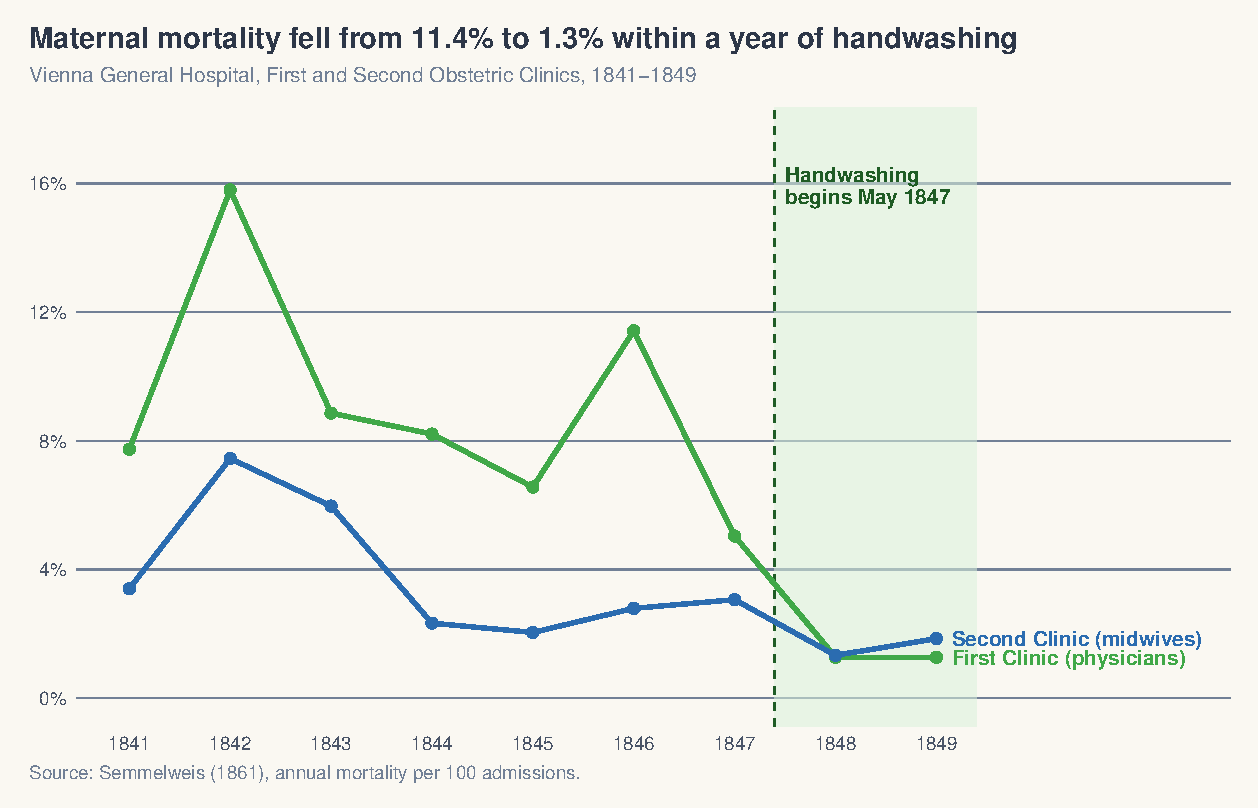
\includegraphics[height=0.72\textheight,keepaspectratio]{figures/semmelweis_remix.pdf}
\end{center}
\begin{center}
\small\color{warmgray}\itshape Monthly mortality, First Obstetric Clinic. Handwashing began mid-1847.
\end{center}
\end{frame}

%% ---------- Slide 15: Semmelweis rejected ----------
\begin{frame}{Rejected}
\vspace{0.4em}
\begin{itemize}
  \item Superiors attributed the drop to a new ventilation system
  \item Miasma theory of disease was still dominant
  \item Semmelweis was passed over for promotion, eventually left Vienna
  \item Published his major treatise in 1861; largely ignored
  \item Committed to an asylum in 1865, died there at 47 --- from infected wounds, the very condition he had been fighting
\end{itemize}
\vspace{0.4em}
\meta{Pasteur and Lister vindicated germ theory in the years that followed.}
\end{frame}

%% =================================================================
%%                  JOHN SNOW
%% =================================================================

%% ---------- Slide 16: Snow setting ----------
\begin{frame}{London, 1854: John Snow vs. miasma}
\vspace{0.4em}
\begin{itemize}
  \item Three cholera waves had hit London since the 1830s
  \item Dominant theory: miasma --- ``foul air''
  \item Snow's theory: a waterborne pathogen, ingested, expelled, recirculated
  \item In 1854, an outbreak gave him a natural experiment
\end{itemize}
\end{frame}

%% ---------- Slide 17: Snow's natural experiment ----------
\begin{frame}{The Metropolis Water Act of 1852}
\vspace{0.4em}
\begin{itemize}
  \item Required London water companies to move their intake pipes upstream, above the city sewage
  \item \highlight{Lambeth} moved its intake to Thames Ditton in 1852 --- clean water
  \item \highlight{Southwark \& Vauxhall} delayed --- still drew from polluted central Thames
  \item Both served overlapping London neighborhoods. Same streets, different water.
\end{itemize}
\end{frame}

%% ---------- Slide 18: Snow's map ----------
\begin{frame}{Customers of two companies, the same streets}
\begin{center}

\includegraphics[height=0.72\textheight,keepaspectratio]{figures/lambeth.png}
\end{center}
\begin{center}
\small\color{warmgray}\itshape Snow walked the streets, recording each household's water company.
\end{center}
\end{frame}

%% ---------- Slide 19: Snow's DiD table — two paths to the same answer ----------
\begin{frame}{Snow's DiD --- two paths to the same number}
\vspace{0.3em}
\begin{center}
\renewcommand{\arraystretch}{1.45}
\begin{tabular}{@{}lcc|c@{}}
\toprule
& \textbf{1849 outbreak} & \textbf{1854 outbreak} & \textbf{Change $\rightarrow$} \\
& \textit{(pre-treatment)} & \textit{(post-treatment)} & \textit{(over time)} \\
\midrule
\textbf{\color{accent}Lambeth} (treated)               & $\overline{Y}_{LB}$ & $\overline{Y}_{LA}$ & $\overline{Y}_{LA} - \overline{Y}_{LB}$ \\
\textbf{\color{slate}Southwark \& Vauxhall} (control)  & $\overline{Y}_{SB}$ & $\overline{Y}_{SA}$ & $\overline{Y}_{SA} - \overline{Y}_{SB}$ \\
\midrule
\textit{Change} $\downarrow$ \textit{(between companies)} & $\overline{Y}_{LB} - \overline{Y}_{SB}$ & $\overline{Y}_{LA} - \overline{Y}_{SA}$ & {\setlength{\fboxsep}{5pt}\colorbox{remixgreenlight}{\textbf{\color{charcoal}$\widehat{\text{DiD}}$}}} \\
\bottomrule
\end{tabular}
\end{center}
\vspace{0.4em}
\begin{center}
\small
$\widehat{\text{DiD}}\;=\;\underbrace{(\overline{Y}_{LA} - \overline{Y}_{LB}) - (\overline{Y}_{SA} - \overline{Y}_{SB})}_{\text{right, then down}}\;=\;\underbrace{(\overline{Y}_{LA} - \overline{Y}_{SA}) - (\overline{Y}_{LB} - \overline{Y}_{SB})}_{\text{down, then right}}$
\end{center}
\vspace{0.2em}
\begin{center}
\small\color{warmgray}\itshape Same four cells. Same answer. Under PT, that number is the ATT for the houses Lambeth supplied.
\end{center}
\end{frame}

%% ---------- Slide: Two paths, two regressions ----------
\begin{frame}[fragile]{The same two paths are two regressions}
\begin{columns}[T,onlytextwidth]
\begin{column}{0.48\textwidth}
{\color{accent}\bfseries\small RIGHT, THEN DOWN}\\[0.3em]
{\scriptsize First-difference each unit, then regress on the treatment dummy.}
\vspace{0.3em}
\begin{enumerate}\scriptsize
  \item $\Delta Y_i = Y_{i,\text{post}} - Y_{i,\text{pre}}$
  \item $\Delta Y_i = \alpha + \delta\,D_i + u_i$
\end{enumerate}
{\scriptsize\color{warmgray}\itshape Slope $\hat\delta$ is the DiD.}
\end{column}
\begin{column}{0.48\textwidth}
{\color{ocean}\bfseries\small DOWN, THEN RIGHT}\\[0.3em]
{\scriptsize Compute the within-period treated-vs-control gap, then regress on Post.}
\vspace{0.3em}
\begin{enumerate}\scriptsize
  \item $G_t = \overline{Y}_{t,\,\text{treat}} - \overline{Y}_{t,\,\text{control}}$
  \item $G_t = \alpha + \delta\,\text{Post}_t + u_t$
\end{enumerate}
{\scriptsize\color{warmgray}\itshape Slope $\hat\delta$ is the same DiD.}
\end{column}
\end{columns}

\vspace{0.4em}
\begin{lstlisting}[language=R,basicstyle=\ttfamily\scriptsize]
# Path 1 -- right then down: unit first-differences on D
wide   <- df |> pivot_wider(names_from = period, values_from = Y)
wide$d <- wide$post - wide$pre
coef(lm(d ~ treat, data = wide))["treat"]      # = DiD

# Path 2 -- down then right: period-level gap on Post
gap    <- df |> group_by(period) |>
            summarize(G = mean(Y[treat == 1]) - mean(Y[treat == 0]))
gap$post <- c(0, 1)
coef(lm(G ~ post, data = gap))["post"]         # = same DiD
\end{lstlisting}
\end{frame}

%% ---------- Slide 20: Snow conclusion ----------
\begin{frame}{Snow identified cholera \textit{before} germ theory}
\vspace{0.4em}
\begin{itemize}
  \item Cholera mortality in Lambeth-supplied houses: a small fraction of Southwark \& Vauxhall houses
  \item The water hypothesis was right --- but the pathogen wouldn't be isolated for another \highlight{29 years} (Koch, 1883)
  \item Snow died in 1858, also before vindication
  \item This is identification by design, decades before the term existed
\end{itemize}
\end{frame}

%% =================================================================
%%                  ASHENFELTER
%% =================================================================

%% ---------- Slide 21a: Princeton Industrial Relations Section ----------
\begin{frame}{Princeton's Industrial Relations Section}
\footnotesize
The Section was older than Princeton's economics department --- founded 1922, with a non-partisan mission: \highlight{rigorous empirical ``manpower'' studies}. \;Worker mobility, unions, wages, federal training programs --- the policy edge of US labor economics.
\vspace{0.3em}
\begin{block}{Orley Ashenfelter's leadership (1970s onward)}
\begin{itemize}
  \item Long-time director. Set the tone: high-quality data, careful design, communicate to bureaucrats.
  \item Trained a remarkable cohort of students through the Section: \\
        \textbf{David Card}, \textbf{Josh Angrist}, \textbf{Bob LaLonde}, \textbf{Janet Currie}, plus Steve Pischke, John Dinardo, Anne Case, and many others.
  \item Hired \textbf{Alan Krueger} as a junior colleague from Harvard --- not a student, but a teammate.
\end{itemize}
\end{block}
\vspace{0.3em}
\begin{center}
\small\color{warmgray}\itshape
A lot of what we now call ``the credibility revolution'' came out of this one floor in Firestone Library.
\end{center}
\end{frame}

%% ---------- Slide 21b: The empirical crisis ----------
\begin{frame}{The empirical crisis that gave us DiD}
\vspace{-0.4em}
\footnotesize
By the late 1970s, empirical labor economics was in trouble. Different methods on the same question \textit{disagreed wildly}. Three pieces crystallized it:
\begin{itemize}
  \item \textbf{LaLonde (1986)} ran the standard methods on a job-training RCT (NSW, ATE $\approx +\$800$) after replacing the experimental control with survey data. Couldn't recover the truth. Methods disagreed by orders of magnitude.
  \item \textbf{Heckman} (\textit{Handbook of Labor Economics}, female labor supply): estimates ``all over the place'' --- many probably weren't credible to begin with.
  \item \textbf{Ashenfelter \& Card (1985, ReStat)}: even DiD wasn't an obvious winner on job training. Honest about its limits from the start.
\end{itemize}
\begin{block}{The Princeton response: design over modeling}
The IRS pushed for estimators that \highlight{mimic an RCT as closely as possible}. DiD was born inside this push --- a step back toward design.
\end{block}
\textbf{Hear Card on the crisis} (26:20): \href{https://youtu.be/1soLdywFb_Q?si=BCVqYeRz6jYiwHTQ&t=1580}{\color{ocean}\texttt{youtu.be/1soLdywFb\_Q?t=1580}}
\end{frame}

%% ---------- Slide 21: Orley's answer — keep it simple ----------
\begin{frame}{Orley's answer: \textit{keep it simple}}
\vspace{0.4em}
\begin{itemize}
  \item Princeton, Industrial Relations Section, late 1970s.
  \item Worker surveys --- matching trainees in federal job-training programs to non-trainees.
  \item Massive panel regressions: \textit{individual} fixed effects $+$ \textit{time} fixed effects.
  \item Audience: federal labor-policy bureaucrats who held the budget.
\end{itemize}
\vspace{0.5em}
\pullquote{Their eyes would glaze over whenever you said `regression.'}{Orley Ashenfelter, in conversation with Scott}
\vspace{0.3em}
\begin{center}
\small\color{warmgray}\itshape
The constraint shaped the method. \;\highlight{DiD was meant to be simple} --- communicable, defensible, transparent. \;Not the most sophisticated estimator on the menu. \;The most useful one.
\end{center}
\end{frame}

%% ---------- Slide 22: His move ----------
\begin{frame}{His move: ``four averages and three subtractions''}
\vspace{0.6em}
\begin{itemize}
  \item Stop leading with the regression
  \item Lead with the thing the regression is computing --- the \highlight{four cell means} and the \highlight{three subtractions} between them
  \item Then, if anyone wants the equation, give them the equation
\end{itemize}
\vspace{0.8em}
\begin{center}
\small\color{warmgray}\itshape Regressions are average-making machines anyway.
\end{center}
\end{frame}

%% ---------- Slide 22b: Hear Orley coin the term ----------
\begin{frame}{Hear Orley coin the term}
\vspace{0.8em}
\begin{itemize}
  \item \textbf{Orley coins ``difference-in-differences''} so he doesn't have to explain regression to bureaucrats. \\[0.4em]
        \href{https://youtu.be/WnB3EJ8K7lg?si=uE4clqUIPzvbxm0r&t=1}{\color{ocean}\texttt{youtu.be/WnB3EJ8K7lg}} \;(3:53 long)
\end{itemize}
\vspace{0.8em}
\begin{center}
\small\color{warmgray}\itshape
Worth hearing in his own voice. The phrase was a rhetorical choice before it was an estimator name.
\end{center}
\end{frame}

%% ---------- Slide 23: The four averages ----------
\begin{frame}{The four averages}
\vspace{0.2em}
\begin{center}
\begin{tikzpicture}
%% Coordinate map:
%% (Y00) at (-2.0, 0.0)  -- control pre
%% (Y10) at (-2.0, -1.5) -- treated pre
%% (Y01) at (2.0, 0.0)   -- control post
%% (Y11) at (2.0, -1.5)  -- treated post

\node[cell] (Y00) at (-2.0, 0.0) {$\overline{Y}_{D=0,\, t=0}$};
\node[cell] (Y01) at (2.0, 0.0) {$\overline{Y}_{D=0,\, t=1}$};
\node[celltreated] (Y10) at (-2.0, -1.5) {$\overline{Y}_{D=1,\, t=0}$};
\node[celltreated] (Y11) at (2.0, -1.5) {$\overline{Y}_{D=1,\, t=1}$};

%% Column headers
\node[anchor=south, font=\small\bfseries, text=charcoal] at (-2.0, 0.75) {Pre ($t=0$)};
\node[anchor=south, font=\small\bfseries, text=charcoal] at (2.0, 0.75) {Post ($t=1$)};

%% Row labels
\node[anchor=east, font=\small\bfseries, text=charcoal] at (-3.7, 0.0) {Control};
\node[anchor=east, font=\small\bfseries, text=accent] at (-3.7, -1.5) {Treated};
\end{tikzpicture}
\end{center}
\vspace{0.5em}
\begin{center}
\small\color{warmgray}\itshape Four cells. Four averages.
\end{center}
\end{frame}

%% ---------- Slide 14: The three subtractions ----------
\begin{frame}{The three subtractions}
\vspace{1.5em}
\begin{center}
\large
\[
\widehat{\text{DiD}} = \underbrace{\big(\overline{Y}_{11} - \overline{Y}_{10}\big)}_{\text{treated change}} \;-\; \underbrace{\big(\overline{Y}_{01} - \overline{Y}_{00}\big)}_{\text{control change}}
\]
\end{center}
\vspace{2em}
\begin{center}
\small\color{warmgray}\itshape
Three subtractions because the outer minus is the third.
\end{center}
\end{frame}

%% ---------- Slide 16: The data (continues Lesson 1) ----------
\begin{frame}{\texttt{castle.dta}: stand-your-ground laws, U.S. states}
\vspace{0.5em}
\begin{itemize}
  \item Cheng \& Hoekstra (2013): did expanding self-defense laws raise homicide rates?
  \item State-year panel
  \item Today: restrict to \highlight{2005--2006} --- a clean 2$\times$2
  \item Treated states: those that adopted in 2006. Control: those that hadn't.
\end{itemize}
\vspace{0.6em}
\meta{Loads directly: \texttt{use https://github.com/scunning1975/mixtape/raw/master/castle.dta}}
\end{frame}

%% ---------- Slide 17: The four cells, Stata ----------
\begin{frame}[fragile]{The four cells, by hand --- in Stata}
\vspace{0.3em}
\begin{lstlisting}[language={[ANSI]C}]
use castle.dta, clear
keep if year >= 2005 & year <= 2006
gen post  = (year == 2006)
gen treat = (effyear == 2006)

* Four cell means
summarize l_homicide if treat==1 & post==1   // Y11
summarize l_homicide if treat==1 & post==0   // Y10
summarize l_homicide if treat==0 & post==1   // Y01
summarize l_homicide if treat==0 & post==0   // Y00
\end{lstlisting}
\end{frame}

%% ---------- Slide 17b: The four cells, R ----------
\begin{frame}[fragile]{The four cells, by hand --- in R}
\vspace{0.3em}
\begin{lstlisting}[language=R]
library(haven); library(dplyr)
df <- read_dta("castle.dta") |>
  filter(year %in% 2005:2006) |>
  mutate(post  = as.integer(year == 2006),
         treat = as.integer(effyear == 2006))

df |>
  group_by(treat, post) |>
  summarize(Ybar = mean(l_homicide), .groups = "drop")
\end{lstlisting}
\end{frame}

%% ---------- Slide 17c: The four cells, Python ----------
\begin{frame}[fragile]{The four cells, by hand --- in Python}
\vspace{0.3em}
\begin{lstlisting}[language=Python]
import pandas as pd
df = pd.read_stata("castle.dta")
df = df.query("year >= 2005 & year <= 2006").copy()
df["post"]  = (df.year == 2006).astype(int)
df["treat"] = (df.effyear == 2006).astype(int)

df.groupby(["treat", "post"])["l_homicide"].mean()
\end{lstlisting}
\end{frame}

%% ---------- Slide 18: The number ----------
\begin{frame}{We get a number. Hold it.}
\vspace{1.5em}
\begin{center}
\Large
$\widehat{\text{DiD}} \;=\; (\overline{Y}_{11} - \overline{Y}_{10}) - (\overline{Y}_{01} - \overline{Y}_{00})$
\end{center}
\vspace{2em}
\begin{center}
\color{warmgray}\itshape
This is the answer. Now we'll get it three more ways.
\end{center}
\end{frame}

%% ---------- Slide 18b: Three languages, one number ----------
\begin{frame}{Same data. Three languages. One number.}
\vspace{0.5em}
\begin{center}
\renewcommand{\arraystretch}{1.5}
\begin{tabular}{@{}lc@{}}
\toprule
\textbf{Stata} & \\
\quad{\ttfamily\small display (y11 - y10) - (y01 - y00)} & \quad $\hat\delta \approx \mathbf{0.10}$ \\
\midrule
\textbf{R} & \\
\quad{\ttfamily\small (Y11 - Y10) - (Y01 - Y00)} & \quad $\hat\delta \approx \mathbf{0.10}$ \\
\midrule
\textbf{Python} & \\
\quad{\ttfamily\small (y11 - y10) - (y01 - y00)} & \quad $\hat\delta \approx \mathbf{0.10}$ \\
\bottomrule
\end{tabular}
\end{center}
\vspace{0.8em}
\begin{center}
\small\color{warmgray}\itshape Log homicide rate is about 10\% higher in 2006-adopting states relative to non-adopting states.\\Stand-your-ground in real numbers.
\end{center}
\end{frame}

%% =====================================================================
%%                                LESSON 3
%% =====================================================================
\remixsection{2.\ Three Regressions, One Answer}

%% ---------- Slide 19b: equivalence pointer ----------
\begin{frame}{Three regressions, three languages}
\vspace{0.8em}
\begin{itemize}
  \item I'll show the \highlight{Stata} version for each of the three specifications
  \item The full multi-language versions are in:
  \begin{itemize}
    \item \texttt{decks/code/equivalence/equivalence.do}
    \item \texttt{decks/code/equivalence/equivalence.R}
    \item \texttt{decks/code/equivalence/equivalence.py}
  \end{itemize}
  \item All three languages, all three regressions, the same number to machine epsilon
\end{itemize}
\end{frame}

%% ---------- Slide 20: OLS with interactions ----------
\begin{frame}[fragile]{Regression 1: OLS with interactions}
\vspace{0.5em}
\begin{lstlisting}[language={[ANSI]C}]
reg l_homicide post##treat, cluster(sid)
\end{lstlisting}
\vspace{1em}
The coefficient on \texttt{1.post\#1.treat} is the DiD.
\vspace{0.5em}
\begin{center}
\small\color{warmgray}\itshape The saturated specification: \quad $Y = \beta_0 + \beta_1\,\text{Post} + \beta_2\,\text{Treat} + \beta_3\,(\text{Post} \times \text{Treat}) + \varepsilon$
\end{center}
\end{frame}

%% ---------- Slide 21: TWFE ----------
\begin{frame}[fragile]{Regression 2: Two-way fixed effects}
\vspace{0.5em}
\begin{lstlisting}[language={[ANSI]C}]
xtset sid year
xtreg l_homicide c.treat#c.post i.year, fe vce(cluster sid)
\end{lstlisting}
\vspace{1em}
State fixed effects absorb time-invariant differences. Year fixed effects absorb common shocks.
\vspace{0.5em}
\begin{center}
\small\color{warmgray}\itshape In the 2$\times$2 case, the TWFE coefficient equals the DiD.\\Tomorrow we'll see when that equivalence breaks.
\end{center}
\end{frame}

%% ---------- Slide 22: Long differences ----------
\begin{frame}[fragile]{Regression 3: Long differences}
\vspace{0.4em}
\begin{lstlisting}[language={[ANSI]C}]
keep sid year l_homicide treat
reshape wide l_homicide, i(sid) j(year)
gen diff = l_homicide2006 - l_homicide2005
reg diff treat, vce(cluster sid)
\end{lstlisting}
\vspace{0.8em}
Collapse to one observation per state. The slope on \texttt{treat} is the DiD.
\vspace{0.4em}
\begin{center}
\small\color{warmgray}\itshape Time-differencing eliminates the unit fixed effects mechanically.
\end{center}
\end{frame}

%% ---------- Slide 23: The same number ----------
\begin{frame}{All three return the same number}
\vspace{1.2em}
\begin{center}
\begin{tabular}{@{}l c@{}}
\textbf{\color{charcoal}Regression 1 (OLS with interactions)} & \color{accent}\textbf{$\widehat{\beta}_3$} \\[0.6em]
\textbf{\color{charcoal}Regression 2 (TWFE)} & \color{accent}\textbf{$\widehat{\beta}_3$} \\[0.6em]
\textbf{\color{charcoal}Regression 3 (Long differences)} & \color{accent}\textbf{$\widehat{\beta}_3$} \\[0.6em]
\textbf{\color{charcoal}Four averages, three subtractions} & \color{accent}\textbf{$\widehat{\beta}_3$} \\
\end{tabular}
\end{center}
\vspace{1em}
\begin{center}
\small\color{warmgray}\itshape Identical to machine epsilon.
\end{center}
\end{frame}

%% ---------- Slide 24: The conjecture ----------
\begin{frame}{This equivalence is what made DiD extensible}
\vspace{0.8em}
\begin{itemize}
  \item OLS infrastructure absorbs covariates, fixed effects, multiple groups, multiple periods
  \item The 2$\times$2 generalizes through the regression
  \item \highlight{But} the equivalence breaks once you add complexity
  \item OLS then needs \textit{additional assumptions} for the coefficients to retain a causal interpretation
\end{itemize}
\vspace{0.5em}
\meta{Tomorrow: covariates, staggered adoption, continuous treatment. Each one breaks something.}
\end{frame}

%% =====================================================================
%%                                LESSON 4
%% =====================================================================
\remixsection{3.\ Potential Outcomes, \\[0.3em] {\normalsize\normalfont Target Parameters, and Parallel Trends}}

%% ---------- Slide 26: Recap — ingredient 1 done ----------
\begin{frame}{Ingredient 1: done. Ingredient 2: now.}
\vspace{0.4em}
\begin{center}
\begin{tikzpicture}
\node[ingredientdone] (calc) at (-3.2,0) {%
  \textcolor{accent}{\large 1. \checkmark} \\[0.3em]
  A \textit{calculation}\\[0.2em]
  \scriptsize\textcolor{warmgray}{(the 2$\times$2)}
};
\node[ingredientpending] (assn) at (3.2,0) {%
  \textcolor{warmgray}{\large 2.\ ?} \\[0.3em]
  An \textit{assumption}\\[0.2em]
  \scriptsize\textcolor{warmgray}{(today)}
};
\node[font=\Large\bfseries,text=accent] at (0,0) {+};
\end{tikzpicture}
\end{center}
\vspace{0.6em}
\begin{center}
\small\color{warmgray}\itshape The calculation gives us a number. The assumption tells us what the number means.
\end{center}
\end{frame}

%% ---------- Slide 27: Angrist anecdote ----------
\begin{frame}{Princeton econometrics, 1980s}
\vspace{0.6em}
\begin{itemize}
  \item Joshua Angrist's recollection: in Princeton's PhD program, potential outcomes were not taught
  \item Econometrics was about \textit{coefficients} --- ``the structure,'' ``the causal effect'' --- not about weighted averages of unit-level effects
  \item The vocabulary that lets us write $Y_i(1) - Y_i(0)$ was \highlight{not yet standard in economics}
\end{itemize}
\end{frame}

%% ---------- Slide 28: Rubin revives Neyman ----------
\begin{frame}{Rubin (1974) revives Neyman (1923)}
\vspace{0.6em}
\begin{itemize}
  \item Jerzy Neyman, 1923 dissertation: introduced potential outcomes notation
  \item Donald Rubin, 1974: ``Estimating Causal Effects of Treatments in Randomized and Nonrandomized Studies''
  \item Together they gave us the explicit language of \highlight{counterfactuals} --- $Y_i(1)$ and $Y_i(0)$ as the two states of the same unit
\end{itemize}
\vspace{0.5em}
\meta{50-year gap. The notation existed before economists started using it.}
\end{frame}

%% ---------- Slide 28b: Individual treatment effect ----------
\begin{frame}{The individual treatment effect}
\vspace{1.4em}
\begin{center}
\Large
\[
\delta_i \;=\; Y_i(1) - Y_i(0)
\]
\end{center}
\vspace{0.6em}
\begin{itemize}
  \item One per unit. \highlight{Different} across units in general --- treatment effects are heterogeneous.
  \item We only ever see one of $Y_i(1)$ or $Y_i(0)$. The other is the counterfactual.
  \item So $\delta_i$ is never directly observed at the individual level.
\end{itemize}
\end{frame}

%% ---------- Slide 28c: Three averages of delta ----------
\begin{frame}{Three averages of $\delta_i$ --- three estimands}
\vspace{0.4em}
All three are expected values. The only difference is \textit{whom we average over}:
\vspace{0.6em}
\begin{itemize}
  \item \textbf{ATE} \;=\; $\mathbb{E}[\delta_i]$ \hfill \meta{average over everyone}
  \item \textbf{ATT} \;=\; $\mathbb{E}[\delta_i \mid D_i = 1]$ \hfill \meta{average over treated units only}
  \item \textbf{ATU} \;=\; $\mathbb{E}[\delta_i \mid D_i = 0]$ \hfill \meta{average over untreated units only}
\end{itemize}
\vspace{1em}
\begin{center}
\small
$\text{ATE} \;=\; \pi \cdot \text{ATT} \;+\; (1-\pi) \cdot \text{ATU}$, \quad where $\pi = \Pr(D=1)$.
\end{center}
\vspace{0.4em}
\begin{center}
\small\color{warmgray}\itshape With heterogeneous effects, the three are different numbers. The one you want depends on the question.
\end{center}
\end{frame}

%% ---------- Slide 28d: 8 people, three averages ----------
\begin{frame}{Eight people, three averages}
\vspace{0.3em}
\begin{center}
\footnotesize
\renewcommand{\arraystretch}{1.1}
\begin{tabular}{@{}c c c c c c@{}}
\toprule
$i$ & $Y_i(0)$ & $Y_i(1)$ & $\delta_i$ & $D_i$ & $Y_i$ (observed) \\
\midrule
\rowcolor{remixgreenlight}1 & 5 & 9  & 4 & 1 & 9 \\
\rowcolor{remixgreenlight}2 & 4 & 10 & 6 & 1 & 10 \\
\rowcolor{remixgreenlight}3 & 6 & 11 & 5 & 1 & 11 \\
\rowcolor{remixgreenlight}4 & 7 & 12 & 5 & 1 & 12 \\
\rowcolor{remixgreenlight}5 & 5 & 8  & 3 & 1 & 8 \\
\midrule
6 & 2 & 3  & 1 & 0 & 2 \\
7 & 3 & 5  & 2 & 0 & 3 \\
8 & 1 & 4  & 3 & 0 & 1 \\
\bottomrule
\end{tabular}
\end{center}
\vspace{0.3em}
\begin{center}
\footnotesize
\textbf{ATE} $= \tfrac{1}{8}(4{+}6{+}5{+}5{+}3{+}1{+}2{+}3) = \mathbf{3.625}$ \quad
\textbf{ATT} $= \tfrac{1}{5}(4{+}6{+}5{+}5{+}3) = \mathbf{4.6}$ \quad
\textbf{ATU} $= \tfrac{1}{3}(1{+}2{+}3) = \mathbf{2.0}$
\end{center}
\vspace{0.1em}
\begin{center}
\footnotesize\color{warmgray}\itshape Three different numbers. If we had both potential outcomes, this is the arithmetic.
\end{center}
\end{frame}

%% ---------- Slide 28e: Which causal effect — weighting ----------
\begin{frame}{Which causal effect do you want? Weighting decides.}
\vspace{0.5em}
\textbf{Solon, Haider \& Wooldridge (2015)}, \textit{What Are We Weighting For?}
\vspace{0.6em}
\begin{itemize}
  \item In a survey, you weight to make estimates \highlight{nationally representative}.
  \item In causal inference, you weight because you want a \highlight{different parameter}.
  \item Different question. Different reason.
\end{itemize}
\vspace{0.6em}
\meta{ATE, ATT, ATU are all expected values. But which expectation? Over which units? With what weights? That's not a survey-design question --- it's a parameter-of-interest question.}
\end{frame}

%% ---------- Slide 28f1: Ten people, two counties — the data ----------
\begin{frame}{Ten people, two counties}
\vspace{0.2em}
\begin{center}
\footnotesize
\renewcommand{\arraystretch}{1.1}
\begin{tabular}{@{}l c c c c@{}}
\toprule
\textbf{Person} & $Y(0)$ & $Y(1)$ & $\delta_i = Y(1)-Y(0)$ & \textbf{County} \\
\midrule
\rowcolor{remixgreenlight}Alan    & 0 & 1 &  1 & 1 \\
\rowcolor{remixgreenlight}Betty   & 1 & 1 &  0 & 1 \\
\rowcolor{remixgreenlight}Chad    & 1 & 1 &  0 & 1 \\
\rowcolor{remixgreenlight}Daniel  & 0 & 0 &  0 & 1 \\
\rowcolor{remixgreenlight}Edith   & 0 & 1 &  1 & 1 \\
\rowcolor{remixgreenlight}Frank   & 0 & 1 &  1 & 1 \\
\rowcolor{remixgreenlight}George  & 0 & 0 &  0 & 1 \\
\rowcolor{remixgreenlight}Hank    & 0 & 1 &  1 & 1 \\
\midrule
\rowcolor{oceanlight}Ida   & 1 & 0 & $-1$ & 2 \\
\rowcolor{oceanlight}Janet & 1 & 0 & $-1$ & 2 \\
\bottomrule
\end{tabular}
\end{center}
\vspace{0.5em}
\begin{center}
\small\color{warmgray}\itshape
County 1: eight people. County 2: two people. Compute the average $\delta$ \\
for each county --- and the average $\delta$ across all ten. Do you get the same answer?
\end{center}
\end{frame}

%% ---------- Slide 28f2: Same data, two weights, two parameters ----------
\begin{frame}{Same data, two weights, two parameters}
\vspace{0.6em}
\begin{itemize}
  \item \textbf{Within counties:} \quad County 1 avg $\delta = \tfrac{1}{8}(1{+}0{+}0{+}0{+}1{+}1{+}0{+}1) = \mathbf{+0.5}$. \\
  \hspace{4.6em} County 2 avg $\delta = \tfrac{1}{2}(-1{+}(-1)) = \mathbf{-1.0}$.
  \item \textbf{ATE for the average person}: $\tfrac{1}{10}(8\cdot 0.5 + 2\cdot(-1)) = \mathbf{+0.2}$
  \item \textbf{ATE for the average county}: $\tfrac{1}{2}(0.5 + (-1)) = \mathbf{-0.25}$
\end{itemize}
\vspace{0.8em}
\begin{center}
\small\color{warmgray}\itshape Same potential outcomes. \highlight{Different signs.} Whichever you report depends on what you're trying to answer.
\end{center}
\end{frame}

%% ---------- Slide 28g: Scaling up the 10-person example ----------
\begin{frame}{Scale it up: 254 counties, 30 million people}
You just saw it with 10 people. Now blow it up. \\
\highlight{Texas}: 254 counties. The 5 biggest (Harris, Dallas, Tarrant, Bexar, Travis) hold 41\% of the population. The other 249 share the rest.
\vspace{0.5em}
\begin{block}{The setup}
\small
Every person has their own treatment effect $\delta_i$. \\[0.15em]
Half: $\delta_i \sim \mathcal{N}(+5,\,1)$. \;\; Half: $\delta_i \sim \mathcal{N}(-1,\,0.5)$. \;\; \highlight{$\mathbb{E}[\delta] = +2$.}
\end{block}
\vspace{0.3em}
We assign people to counties \textit{two} different ways:
\begin{itemize}\small
  \item[$\blacktriangleright$] \textbf{Random} --- each county is a random sample of the population.
  \item[$\blacktriangleright$] \textbf{Sort by $\delta$} --- high-effect people end up in the 5 big counties.
\end{itemize}
\meta{The $\delta_i$ values are identical in both scenarios. Only who-lives-where changes.}
\end{frame}

%% ---------- Slide 28h: Sorting matters — the picture ----------
\begin{frame}{Sorting on $\delta$ can flip the sign of your answer}
\begin{center}
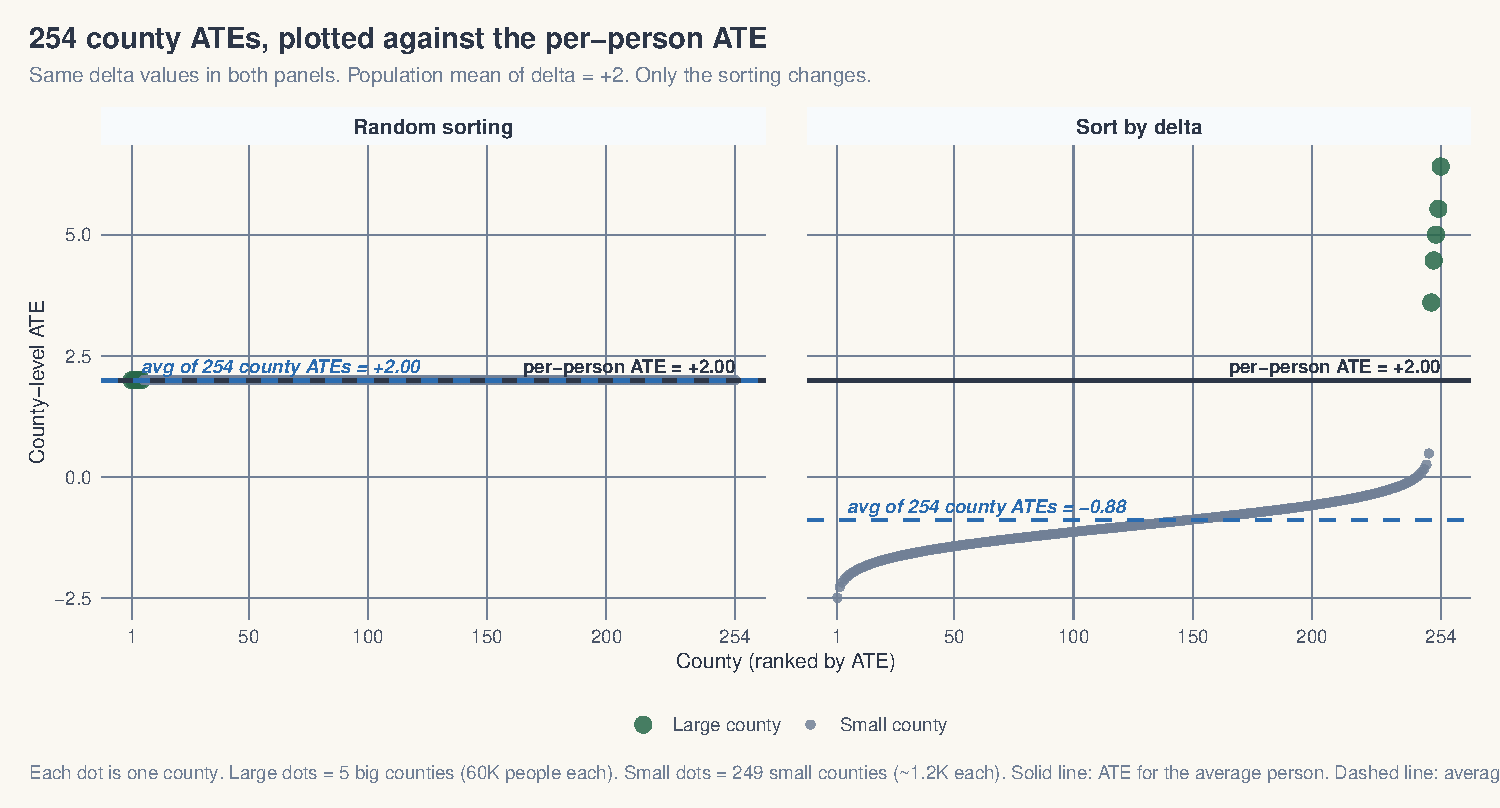
\includegraphics[width=0.92\linewidth,height=0.68\textheight,keepaspectratio]{figures/tiebout_roy_distributions.pdf}
\end{center}
\vspace{-0.3em}
\begin{center}
\scriptsize\color{warmgray}\itshape
Random: every county's ATE equals the population's. \;\;
$\delta$-sort: per-person line at $+2$, avg of county ATEs flips to \highlight{$-0.88$.} \\[0.15em]
Random sorting is the benchmark --- rarely reality. People choose where to live, and on traits that move $\delta$.
\end{center}
\end{frame}

%% ---------- Slide 28h2: Why the sign flips ----------
\begin{frame}{Two parameters, two answers}
\vspace{0.4em}
Under $\delta$-sort, the 5 big counties cluster at $\approx +5$. The 249 small counties cluster at $\approx -1$.
\vspace{0.6em}
\begin{itemize}\small
  \item \textbf{Per-person ATE}: \;$\tfrac{1}{N}\sum_i \delta_i$ --- weight every person by $1/N$. \\[0.2em]
        The 15M high-$\delta$ people balance the 15M low-$\delta$ people. \;\highlight{Answer: $+2$.}
  \item \textbf{Avg of county ATEs}: $\tfrac{1}{254}\sum_c \overline{\delta}_c$ --- weight every county by $1/254$. \\[0.2em]
        $\tfrac{5(+5) + 249(-1)}{254} = \;\highlight{-0.88}$. \; The 249 small counties dominate.
\end{itemize}
\vspace{0.6em}
\begin{center}
\small\color{warmgray}\itshape
Same data. Two weights. Two parameters. Sometimes two signs.
\end{center}
\end{frame}

%% ---------- Slide 28h3: What this means for DiD ----------
\begin{frame}{What this means for DiD on aggregate data}
DiD usually runs on aggregates: counties, states, hospitals.
\begin{itemize}\small
  \item Equal weights per unit $\Rightarrow$ \textbf{unit-weighted ATE}: the effect for the average \textit{location}.
  \item Weight by population $\Rightarrow$ \textbf{person-weighted ATE}: the effect for the average \textit{person}.
\end{itemize}
\vspace{0.3em}
\begin{block}{Which one you want depends on the question}
\small
\textit{Person-weighted} for \highlight{aggregate human welfare}: how many people are affected, by how much? \\[0.2em]
\textit{Unit-weighted} when locations have \highlight{autonomy and goals}: each policy unit chooses independently --- the unit \textit{is} the agent.
\end{block}
\vspace{0.1em}
\meta{Solon, Haider \& Wooldridge (2015). Code: \texttt{decks/code/Tiebout-Roy/tiebout\_roy\_chart.R}}
\end{frame}

%% ---------- Slide 28h4: The weighted mean — one formula ----------
\begin{frame}{The weighted mean --- a single formula}
\vspace{0.5em}
\begin{center}
\Large
\[
\overline{Y}_w \;=\; \frac{\sum_i w_i\,Y_i}{\sum_i w_i}
\]
\end{center}

\vspace{1em}
The weight is the choice:
\begin{itemize}\setlength\itemsep{6pt}
  \item $w_i = 1$ for every unit $\;\Rightarrow\;$ \highlight{unit-weighted} (the average county).
  \item $w_i =$ population $\;\Rightarrow\;$ \highlight{person-weighted} (the average person).
\end{itemize}
\end{frame}

%% ---------- Slide 28h5: Two DiDs on the same 10 people ----------
\begin{frame}{Two weights, two signs}
\vspace{0.4em}
\textbf{Same 10 people.} \;County 1 DiD $= +0.5$ (8 people). \;County 2 DiD $= -1.0$ (2 people).

\vspace{1em}
\begin{center}
\textbf{Person-weighted:} \;\;
$\dfrac{8 \cdot (+0.5) + 2 \cdot (-1.0)}{8 + 2} \;=\; \mathbf{+0.2}$
\end{center}

\vspace{0.5em}
\begin{center}
\textbf{Unit-weighted:} \;\;
$\dfrac{(+0.5) + (-1.0)}{2} \;=\; \mathbf{-0.25}$
\end{center}

\vspace{1em}
\begin{center}
\highlight{Same data. Different weight. Different sign.}
\end{center}
\end{frame}

%% ---------- Slide 28h6a: Castle data, manual weighted 2x2 — Stata ----------
\begin{frame}[fragile]{Castle data: the weighted 2$\times$2 by hand}
\footnotesize
Four cell means, each with \texttt{[aw=popwt]}:
\vspace{0.2em}
\begin{lstlisting}[language={[ANSI]C},basicstyle=\ttfamily\scriptsize]
summarize l_homicide if treat==1 & post==1 [aw=popwt]
gen wy11 = `r(mean)'
summarize l_homicide if treat==1 & post==0 [aw=popwt]
gen wy10 = `r(mean)'
summarize l_homicide if treat==0 & post==1 [aw=popwt]
gen wy01 = `r(mean)'
summarize l_homicide if treat==0 & post==0 [aw=popwt]
gen wy00 = `r(mean)'

gen wdid = (wy11 - wy10) - (wy01 - wy00)
display wdid          // 0.0964
\end{lstlisting}
\end{frame}

%% ---------- Slide 28h6b: Same number via Stata regression ----------
\begin{frame}[fragile]{Same number via regression: Stata}
\vspace{0.6em}
\begin{lstlisting}[language={[ANSI]C},basicstyle=\ttfamily\small]
reg l_homicide post##treat [aweight=popwt], cluster(sid)
\end{lstlisting}

\vspace{0.8em}
\begin{center}
Coefficient on \texttt{1.post\#1.treat} $\;=\; \mathbf{0.0964}$
\end{center}

\vspace{1em}
\begin{center}
\small\color{warmgray}\itshape \texttt{aweight} \textit{is} the formula --- run inside OLS.
\end{center}
\end{frame}

%% ---------- Slide 28h7: Same number via R ----------
\begin{frame}[fragile]{Same number via regression: R}
\vspace{0.6em}
\begin{lstlisting}[language=R,basicstyle=\ttfamily\small]
library(fixest)

feols(l_homicide ~ post * treat,
      data    = castle,
      weights = ~popwt,
      cluster = ~sid)
\end{lstlisting}

\vspace{0.8em}
\begin{center}
Coefficient on \texttt{post:treat} $\;=\; \mathbf{0.0964}$
\end{center}
\end{frame}

%% ---------- Slide 28h8: Same number via Python ----------
\begin{frame}[fragile]{Same number via regression: Python}
\vspace{0.6em}
\begin{lstlisting}[language=Python,basicstyle=\ttfamily\small]
import statsmodels.formula.api as smf

mod = smf.wls("l_homicide ~ post * treat",
              data    = castle,
              weights = castle["popwt"]).fit(
        cov_type = "cluster",
        cov_kwds = {"groups": castle["sid"]})
\end{lstlisting}

\vspace{0.8em}
\begin{center}
\texttt{mod.params["post:treat"]} $\;=\; \mathbf{0.0964}$
\end{center}
\end{frame}

%% ---------- Slide 29a: From parameter choice to ATT ----------
\begin{frame}{Pick a target parameter}
\vspace{0.6em}
Everything until now has been about \textit{parameters}: ATE, ATT, ATU.
\vspace{0.3em}
\begin{itemize}
  \item Three weights. Three signs. Three answers.
  \item The choice is about \textit{which causal effect you actually want}.
\end{itemize}

\vspace{1.2em}
\begin{center}
\Large\highlight{Today's target: the ATT.}
\end{center}

\vspace{0.8em}
\begin{center}
\small\color{warmgray}\itshape The average effect for the units that actually received the treatment.
\end{center}
\end{frame}

%% ---------- Slide 29b: The switching equation ----------
\begin{frame}{The switching equation: you see one half}
\vspace{0.8em}
\begin{center}
\Large
\[
Y_i \;=\; D_i \cdot Y_i(1) \;+\; (1 - D_i) \cdot Y_i(0)
\]
\end{center}

\vspace{1em}
\begin{itemize}\setlength\itemsep{6pt}
  \item For each unit: $Y_i(1)$ if treated, $Y_i(0)$ if not.
  \item ATT asks about \textit{both} columns. The data hands you one.
\end{itemize}

\vspace{0.8em}
\meta{The rest of the day: strategies for recovering the ATT from the half you see.}
\end{frame}

%% ---------- Slide 29a1: SDO calculation ----------
\begin{frame}{What if we just compared $Y$ between treated and untreated?}
\vspace{0.5em}
The simple difference in observed outcomes (SDO):
\vspace{0.5em}
\[
\text{SDO} \;=\; \mathbb{E}[Y_i \mid D_i = 1] - \mathbb{E}[Y_i \mid D_i = 0]
\]
\vspace{0.4em}
For our 8 people:
\[
\text{SDO} \;=\; \tfrac{1}{5}(9{+}10{+}11{+}12{+}8) - \tfrac{1}{3}(2{+}3{+}1) \;=\; 10 - 2 \;=\; \mathbf{8}
\]
\vspace{0.4em}
\begin{center}
But ATT $= 4.6$. ATE $= 3.625$. ATU $= 2.0$.\\[0.3em]
\highlight{The SDO is bigger than any of them.}
\end{center}
\end{frame}

%% ---------- Slide 29a2: SDO = ATT + selection bias ----------
\begin{frame}{SDO $=$ ATT $+$ selection bias}
\vspace{0.3em}
Add and subtract $\mathbb{E}[Y_i(0) \mid D_i = 1]$ inside the SDO and rearrange:
\vspace{0.3em}
\begin{align*}
\underbrace{\mathbb{E}[Y \mid D=1] - \mathbb{E}[Y \mid D=0]}_{\text{SDO}}
 \;=\;& \underbrace{\mathbb{E}[Y(1) - Y(0) \mid D=1]}_{\textstyle\text{\color{accent}\bfseries ATT}} \\[0.4em]
 +\;& \underbrace{\mathbb{E}[Y(0) \mid D=1] - \mathbb{E}[Y(0) \mid D=0]}_{\text{\bfseries selection bias}}
\end{align*}
\vspace{0.1em}

In the 8-person example:\\[0.2em]
selection bias $=\; \tfrac{1}{5}(5{+}4{+}6{+}7{+}5) - \tfrac{1}{3}(2{+}3{+}1) \;=\; 5.4 - 2.0 \;=\; \mathbf{3.4}$\\[0.4em]
SDO $= 4.6 + 3.4 = 8$ \quad\checkmark
\end{frame}

%% ---------- Slide 29a3: Calculations alone aren't enough ----------
\begin{frame}{Calculations alone aren't enough}
\vspace{0.5em}
\begin{itemize}
  \item The SDO is something we can \textit{always} calculate from the data.
  \item It is the population estimand of the naive comparison.
  \item But it is \highlight{not the target parameter} --- in general, SDO $\neq$ ATT $\neq$ ATE $\neq$ ATU.
  \item The gap is the selection bias. It does not go away by collecting more data.
\end{itemize}
\vspace{0.6em}
\begin{block}{To turn a calculation into a causal target, we need an \textit{identification strategy}}
RCT: random assignment makes selection bias zero. \\
IV: relevance + exclusion. \\
RDD: continuity at the cutoff. \\
\highlight{DiD: parallel trends + no anticipation + stability (SUTVA).}
\end{block}
\end{frame}

%% ---------- Slide 29b: Bridge — causal inference ↔ statistics ----------
\begin{frame}{Let's connect causal inference with statistics for a second}
\vspace{0.6em}
\begin{itemize}
  \item So far the language has been \textit{causal}: $Y(1)$, $Y(0)$, the switching equation, the counterfactual.
  \item Causal claims are about \highlight{populations} --- the average effect on the treated, $\mathbb{E}[Y(1) - Y(0) \mid D = 1]$.
  \item But we never see the population. We see a sample.
  \item Which means we need the \textit{statistical} layer too: sampling distributions, estimators, convergence.
\end{itemize}
\vspace{0.6em}
\meta{The two layers interlock --- one tells us what we want to estimate; the other tells us how close our estimate gets.}
\end{frame}

%% ---------- Slide 30: All the data thought experiment ----------
\begin{frame}{Suppose you had all the data}
\vspace{1.5em}
\begin{center}
\large
\color{charcoal}What would you compute?
\end{center}
\vspace{2em}
\begin{center}
\small\color{warmgray}\itshape A regression. A difference of means. A ratio. \\Whatever the data permits.
\end{center}
\end{frame}

%% ---------- Slide 31: Population estimand ----------
\begin{frame}{That's a \textit{population estimand}}
\vspace{0.6em}
\begin{block}{Population estimand}
The calculation you could do if you had the entire population. \\[0.4em]
A function of population moments --- means, variances, regressions. \\[0.4em]
\highlight{Not} a sample quantity. \highlight{Not} necessarily causal.
\end{block}
\vspace{0.6em}
\meta{Sometimes denoted $\theta$. The thing your estimator is converging to in the limit.}
\end{frame}

%% ---------- Slide 31b: Two layers ----------
\begin{frame}{Shape is statistics. Center is identification.}
\begin{center}
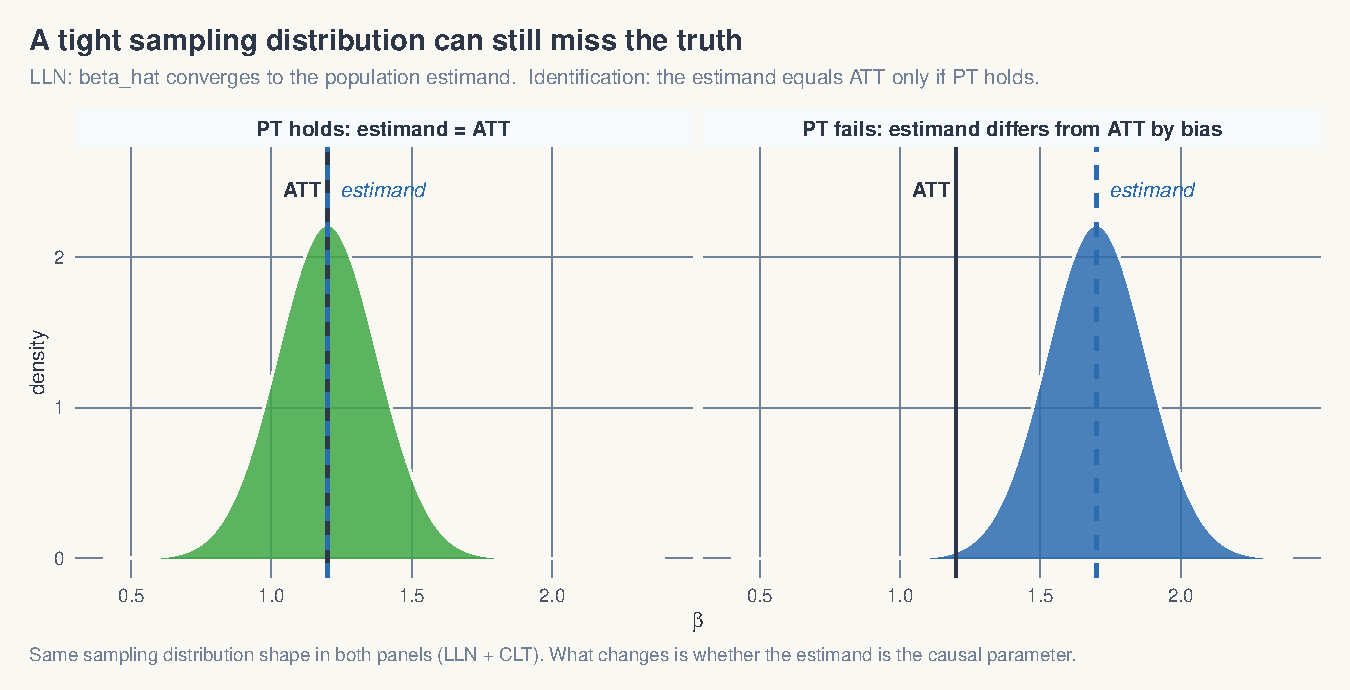
\includegraphics[height=0.60\textheight,keepaspectratio]{figures/sampling_distribution.pdf}
\end{center}
\footnotesize
\textbf{\color{accent}Shape} of the sampling distribution $\leftarrow$ LLN + CLT. Independent of whether the design is causal.\\
\textbf{\color{ocean}Center} of the sampling distribution $\leftarrow$ identification. Equals ATT only if PT holds.\\
\highlight{Same data, same estimator, same statistics --- two completely different conclusions.}
\end{frame}

%% ---------- Slide 32: Regress earnings on college ----------
\begin{frame}{Regress earnings on a college dummy. Causal?}
\vspace{1.8em}
\begin{center}
\Large
\[
\beta \;=\; \mathbb{E}[\,\text{Earnings} \mid \text{College} = 1\,] \;-\; \mathbb{E}[\,\text{Earnings} \mid \text{College} = 0\,]
\]
\end{center}
\vspace{1em}
\begin{center}
\color{charcoal}Is $\beta$ the causal effect of college?
\end{center}
\end{frame}

%% ---------- Slide 33: Yes if randomized; no if selection ----------
\begin{frame}{Yes if randomized. No if selection.}
\vspace{0.6em}
\begin{center}
\begin{tikzpicture}
\node[conceptbox=accent] (rand) at (-3.5, 0) {%
  \textbf{\color{accent}Randomized}\\[0.3em]
  \small Treatment assigned by coin flip. Treated and untreated populations are identical in expectation.\\[0.3em]
  \small $\beta$ \textit{is} the causal effect.
};
\node[conceptbox=warmgray] (sel) at (3.5, 0) {%
  \textbf{\color{warmgray}Selection}\\[0.3em]
  \small College-goers differ from non-college-goers in ability, family background, ambition.\\[0.3em]
  \small $\beta$ is biased.
};
\end{tikzpicture}
\end{center}
\end{frame}

%% ---------- Slide 34: Biased estimand vs unbiased target parameter ----------
\begin{frame}{An estimand can be biased. A target parameter cannot.}
\vspace{0.5em}
\begin{block}{Population estimand}
What the math gives you with all the data. \\
Sometimes equals the causal effect. Sometimes doesn't.
\end{block}
\vspace{-0.5em}
\begin{alertblock}{Target parameter}
The causal object you actually want. \\
Defined in potential-outcomes notation. \\
\highlight{Unbiased by construction} --- it \textit{is} the causal effect.
\end{alertblock}
\end{frame}

%% ---------- Slide 35: Bias = non-causal terms ----------
\begin{frame}{Bias is what rides along with the causal term}
\vspace{1.5em}
\begin{center}
\large
\[
\underbrace{\text{Estimand}}_{\text{what the math gives}} \;=\; \underbrace{\text{Causal term}}_{\text{target parameter}} \;+\; \underbrace{\text{Bias}}_{\text{everything else}}
\]
\end{center}
\vspace{1.5em}
\begin{center}
\small\color{warmgray}\itshape
Bias is the gap. Sometimes zero (randomization). Often not.
\end{center}
\end{frame}

%% ---------- Slide 36: Identification strips the bias ----------
\begin{frame}{Identification strips the bias}
\vspace{0.4em}
\begin{itemize}
  \item Identification = a set of assumptions under which the bias term vanishes
  \item With those assumptions, the population estimand \highlight{equals} the target parameter
  \item Different designs use different identifying assumptions:
  \begin{itemize}
    \item Randomization $\rightarrow$ ATE
    \item \highlight{Parallel trends $\rightarrow$ ATT}
    \item Instrumental variables $\rightarrow$ LATE
    \item Regression discontinuity $\rightarrow$ local ATE
  \end{itemize}
\end{itemize}
\end{frame}

%% ---------- Slide 37: ATT is the target parameter ----------
\begin{frame}{The ATT is the DiD target parameter}
\vspace{1.5em}
\begin{center}
\Large
\[
\text{ATT} \;=\; \mathbb{E}\big[\, Y_i(1) - Y_i(0) \;\big|\; D_i = 1,\; t = \text{Post}\,\big]
\]
\end{center}
\vspace{1em}
\begin{center}
\color{charcoal}The average treatment effect on the treated, after treatment.
\end{center}
\vspace{0.6em}
\meta{Treated units. Post-treatment period. Not the ATE.}
\end{frame}

%% ---------- Slide 38: The proof — add a zero (5 steps) ----------
\begin{frame}{The proof: add a zero, rearrange (five steps)}
\vspace{-0.4em}
\footnotesize

\textbf{1. Start with the 2$\times$2 calculation} (four cell means, three subtractions):
\vspace{-0.6em}
\[
\widehat{\text{DiD}} \;=\; \big[\mathbb{E}[Y\mid D{=}1,\text{Post}] - \mathbb{E}[Y\mid D{=}1,\text{Pre}]\big]
                    \;-\; \big[\mathbb{E}[Y\mid D{=}0,\text{Post}] - \mathbb{E}[Y\mid D{=}0,\text{Pre}]\big]
\]
\vspace{-1.1em}

\textbf{2. Apply the switching equation} $Y = D\,Y(1) + (1{-}D)\,Y(0)$. Treated-post is $Y(1)$; the other three cells are $Y(0)$:
\vspace{-0.3em}
\[
\widehat{\text{DiD}} \;=\; \big[\mathbb{E}[Y(1)\mid 1,\text{Post}] - \mathbb{E}[Y(0)\mid 1,\text{Pre}]\big]
                    \;-\; \big[\mathbb{E}[Y(0)\mid 0,\text{Post}] - \mathbb{E}[Y(0)\mid 0,\text{Pre}]\big]
\]
\vspace{-0.4em}

\textbf{3. Add a zero.} \;Insert $+\,\mathbb{E}[Y(0)\mid 1,\text{Post}] \;-\; \mathbb{E}[Y(0)\mid 1,\text{Post}]$ (the missing counterfactual for the treated group):
\vspace{-0.3em}
\begin{align*}
\widehat{\text{DiD}} \;=\;&
  \mathbb{E}[Y(1)\mid 1,\text{Post}] \;-\; \mathbb{E}[Y(0)\mid 1,\text{Post}] \\
& {} +\;\mathbb{E}[Y(0)\mid 1,\text{Post}] - \mathbb{E}[Y(0)\mid 1,\text{Pre}]
   \;-\; \big[\mathbb{E}[Y(0)\mid 0,\text{Post}] - \mathbb{E}[Y(0)\mid 0,\text{Pre}]\big]
\end{align*}
\vspace{-0.4em}

\textbf{4. Rearrange.} \;First two terms = ATT; rest = a difference of differences in $Y(0)$ trends:
\vspace{-0.3em}
\[
\widehat{\text{DiD}} \;=\; \underbrace{\mathbb{E}[Y(1) - Y(0)\mid 1,\text{Post}]}_{\textstyle\text{\color{accent}\bfseries ATT}}
                    \;+\; \underbrace{\big\{\Delta\mathbb{E}[Y(0)\mid 1] \;-\; \Delta\mathbb{E}[Y(0)\mid 0]\big\}}_{\textstyle\text{non-parallel-trends bias}}
\]
\vspace{-0.4em}

\textbf{5. Read.} If the bias equals zero (\textit{parallel trends}), then $\widehat{\text{DiD}} = \text{ATT}$.
\end{frame}

%% ---------- Slide 38b: The bias IS selection bias on Y(0) trends ----------
\begin{frame}{The bias term \textit{is} selection bias --- on trends, not levels}
\footnotesize
The ``non-parallel-trends bias'' isn't a new concept. It's selection bias, in a different costume.
\vspace{-0.5em}
\[
\text{bias} \;=\; \underbrace{\Delta\mathbb{E}[Y(0)\mid D{=}1]}_{\text{how treated's $Y(0)$ moves}} \;-\; \underbrace{\Delta\mathbb{E}[Y(0)\mid D{=}0]}_{\text{how controls' $Y(0)$ moves}}
\]
\vspace{-0.4em}
\begin{itemize}
  \item \textbf{Cross-section selection bias} asks: are treated and control different in \textit{levels} of $Y(0)$?
  \item \textbf{DiD's selection bias} asks: are treated and control different in \textit{trends} of $Y(0)$?
  \item Different levels are fine. Unit fixed effects soak them up.
  \item What \textit{can't} differ is the \textit{rate} at which $Y(0)$ moves across groups. If it does, the DiD reports the gap as treatment effect.
\end{itemize}
\vspace{0.2em}
\begin{block}{The trade DiD makes vs.\ randomization}
RCTs: treated and controls identical in everything --- levels and trends. \\
DiD: treated and controls only need to be identical in \textit{trends} of $Y(0)$. \;\highlight{Cheaper assumption. Weaker identification.}
\end{block}
\end{frame}

%% =========================================================================
%% Slides 38c1–38c6: Four ways the 2x2 can go wrong (case decomposition tour)
%% =========================================================================

%% ---------- Slide 38c1: Section intro ----------
\begin{frame}{Four ways the 2$\times$2 can go wrong}
\footnotesize
The proof on the last slide identifies the ATT \textbf{only} when three things hold:
\begin{enumerate}\setlength\itemsep{2pt}
  \item[\textbf{(i)}] \highlight{No Anticipation (NA)} --- pre-period $Y$ for the treated group equals $Y(0)$
  \item[\textbf{(ii)}] \highlight{Parallel Trends (PT)} --- $Y(0)$ moves the same way in both groups
  \item[\textbf{(iii)}] The comparison group is itself \highlight{untreated}
\end{enumerate}

\vspace{0.4em}
Four scenarios. The same \textbf{+0 trick} works on all of them --- only the zero you add changes.
\vspace{-0.3em}
\begin{itemize}\setlength\itemsep{2pt}
  \item \textbf{Case 1.}\; NA \checkmark, never-treated control \checkmark \hfill $\widehat{\text{DiD}} = \text{ATT}$
  \item \textbf{Case 2.}\; \textbf{NA fails}, never-treated control \hfill $\widehat{\text{DiD}} = \text{ATT} - \text{ATT}_{\text{pre}}$
  \item \textbf{Case 3.}\; NA \checkmark, but control absorbs \textbf{spillover} \hfill $\widehat{\text{DiD}} = \text{ATT} - \text{spillover}$
  \item \textbf{Case 4.}\; NA \checkmark, but control is \textbf{already-treated} \hfill $\widehat{\text{DiD}} = \text{ATT} - \Delta\text{ATT}$
\end{itemize}

\vspace{0.3em}
\meta{Each case: the +0 trick, a numerical example, a Monte Carlo verdict at the end.}
\end{frame}

%% ---------- Slide 38c2: Case 1 — NA + never-treated ----------
\begin{frame}{Case 1.\ NA holds, never-treated comparison}
\footnotesize
\textbf{Switching equation.} \;Treated-post is $Y(1)$; the other three cells are $Y(0)$.
\vspace{-0.2em}
\[
\widehat{\text{DiD}} \;=\; \big[\mathbb{E}[Y(1)|1,\text{Post}] - \mathbb{E}[Y(0)|1,\text{Pre}]\big]
                  \;-\; \big[\mathbb{E}[Y(0)|0,\text{Post}] - \mathbb{E}[Y(0)|0,\text{Pre}]\big]
\]
\vspace{-1.1em}

\textbf{Add the zero.} \;Insert $+\,\mathbb{E}[Y(0)|1,\text{Post}] - \mathbb{E}[Y(0)|1,\text{Post}]$. \;Rearrange:
\vspace{-0.3em}
\[
\widehat{\text{DiD}} \;=\; \underbrace{\mathbb{E}[Y(1)-Y(0)|1,\text{Post}]}_{\textstyle\text{\color{accent}\bfseries ATT}}
                  \;+\; \underbrace{\big\{\Delta\mathbb{E}[Y(0)|1] - \Delta\mathbb{E}[Y(0)|0]\big\}}_{\text{non-PT bias}\;=\;0\;\text{under PT}}
\]
\vspace{-0.6em}

\begin{block}{Numerical example}
ATT $= 10$, \;PT bias $= 0$. \quad $\widehat{\text{DiD}} = \mathbf{10}$. \;\checkmark
\end{block}
\meta{Monte Carlo (2000 reps, $n=200$/group, $\sigma=2$): mean $\widehat{\text{DiD}} = 10.005$.}
\end{frame}

%% ---------- Slide 38c3: Case 2 — NA fails ----------
\begin{frame}{Case 2.\ NA fails --- anticipation contaminates $Y_{\text{Pre}}$}
\footnotesize
Suppose the treated group anticipates and adjusts \textit{before} the policy lands. Then their pre-period outcome contains some $Y(1)$ response: \;$\mathbb{E}[Y|1,\text{Pre}] = \mathbb{E}[Y(0)|1,\text{Pre}] + \textcolor{accent}{\text{ATT}_{\text{pre}}}$.

\vspace{0.3em}
\textbf{Same +0 trick}, propagated:
\vspace{-0.3em}
\[
\widehat{\text{DiD}} \;=\; \underbrace{\text{ATT}_{\text{Post}}}_{\text{what we want}}
                  \;+\; \underbrace{\text{non-PT bias}}_{=\,0}
                  \;-\; \underbrace{\textcolor{accent}{\text{ATT}_{\text{pre}}}}_{\text{anticipation}}
\]
\vspace{-0.6em}

\begin{block}{Numerical example}
ATT $= 10$, \;PT bias $= 0$, \;ATT$_{\text{pre}} = 3$. \quad $\widehat{\text{DiD}} = 10 - 3 = \mathbf{7}$. \;\highlight{biased down}
\end{block}
\meta{Monte Carlo: mean $\widehat{\text{DiD}} = 7.01$. \;If treatment effects are roughly constant, DiD can collapse to zero.}
\end{frame}

%% ---------- Slide 38c4: Case 3 — spillover ----------
\begin{frame}{Case 3.\ Spillover --- the control group absorbs $Y(1)$ in Post}
\footnotesize
Suppose the policy spills onto the comparison group in the post period (general-equilibrium, displacement, social interaction). Then \;$\mathbb{E}[Y|0,\text{Post}] = \mathbb{E}[Y(0)|0,\text{Post}] + \textcolor{accent}{\text{spillover}}$.

\vspace{0.3em}
\textbf{Same recipe} --- the zero you add lives on the control side, not the treated side:
\vspace{-0.3em}
\[
\widehat{\text{DiD}} \;=\; \underbrace{\text{ATT}}_{\text{what we want}}
                  \;+\; \underbrace{\text{non-PT bias}}_{=\,0}
                  \;-\; \underbrace{\textcolor{accent}{\text{spillover}}}_{\text{control got treated too}}
\]
\vspace{-0.6em}

\begin{block}{Numerical example}
ATT $= 10$, \;PT bias $= 0$, \;spillover $= 4$. \quad $\widehat{\text{DiD}} = 10 - 4 = \mathbf{6}$. \;\highlight{biased toward zero}
\end{block}
\meta{Monte Carlo: mean $\widehat{\text{DiD}} = 6.01$. \;The Stable Unit Treatment Value Assumption (SUTVA) failed --- the ``control'' wasn't really untreated.}
\end{frame}

%% ---------- Slide 38c5: Case 4 — already-treated control ----------
\begin{frame}{Case 4.\ The forbidden 2$\times$2 --- already-treated comparison}
\footnotesize
Now the ``comparison'' group was treated \textit{before} the pre-period. Both their pre and post cells are $Y(1)$, with effects that can move over time: \;$\Delta\text{ATT} \equiv \text{ATT}(\text{Post},D{=}0) - \text{ATT}(\text{Pre},D{=}0)$.

\vspace{0.2em}
\textbf{Same recipe, three zeros} (one per $Y(0)$ counterfactual we need):
\vspace{-0.3em}
\[
\widehat{\text{DiD}} \;=\; \underbrace{\text{ATT}}_{\text{what we want}}
                  \;+\; \underbrace{\text{non-PT bias}}_{=\,0}
                  \;-\; \underbrace{\textcolor{accent}{\Delta\text{ATT}}}_{\text{control's effect dynamics}}
\]
\vspace{-0.7em}

\textbf{Two numerical examples.}\;ATT$=10$, PT bias$=0$:
\vspace{-0.2em}
\begin{itemize}\setlength\itemsep{1pt}
  \item Control's ATT(Pre)$=1$, ATT(Post)$=5$, $\Delta\text{ATT}=4$: \;$\widehat{\text{DiD}} = 10-4 = \mathbf{6}$
  \item Control's ATT(Pre)$=1$, ATT(Post)$=15$, $\Delta\text{ATT}=14$: \;$\widehat{\text{DiD}} = 10-14 = \mathbf{-4}$ \;\highlight{sign flip}
\end{itemize}

\begin{block}{The Bacon insight}
The forbidden 2$\times$2 identifies $-\Delta\text{ATT}$. \;If treatment effects \textbf{grow over time}, DiD reports the \textit{wrong sign}. \;Foreshadows Bacon (2021), tomorrow.
\end{block}
\end{frame}

%% ---------- Slide 38c6: The Monte Carlo verdict ----------
\begin{frame}{Monte Carlo verdict --- 2000 reps, four cases, one truth}
\vspace{-0.2em}
\begin{center}
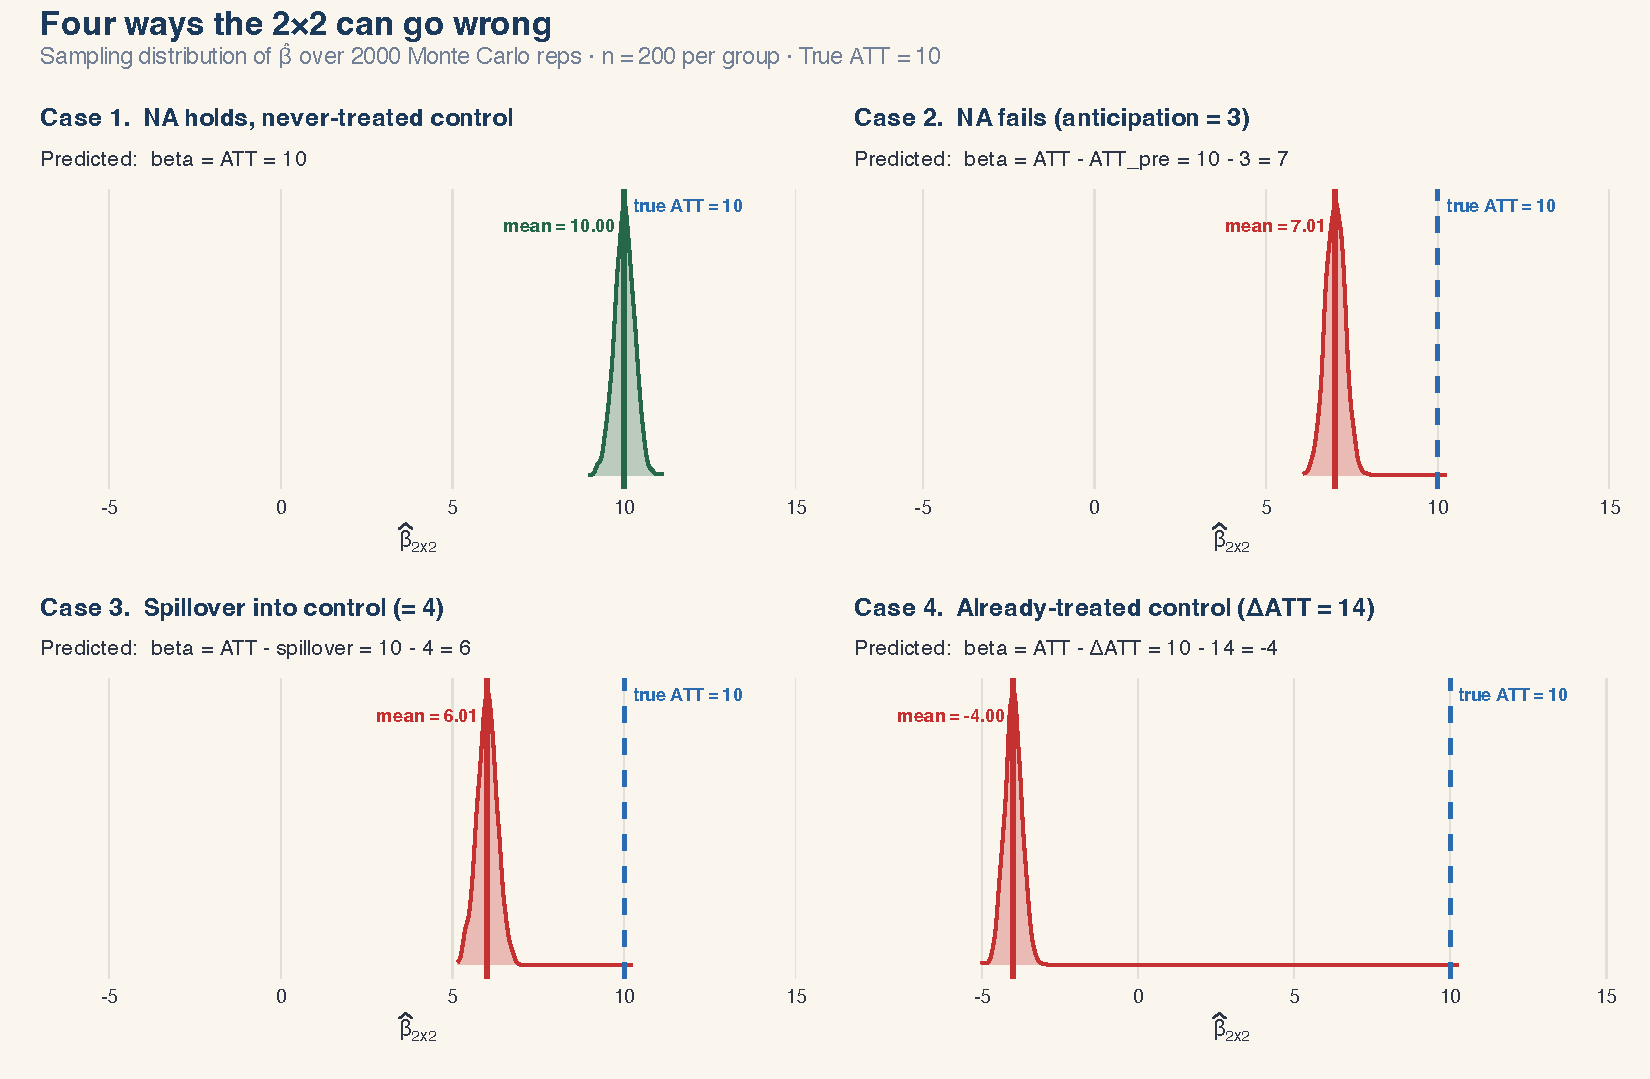
\includegraphics[height=0.74\textheight,keepaspectratio]{figures/case_decompositions.pdf}
\end{center}
\vspace{-0.4em}
\meta{Only Case 1 puts the truth at the center of the sampling distribution. The other three are sharp, narrow, and \textit{wrong}.}
\end{frame}

%% =========================================================================
%% Slides 38d1–38d5: Preview of Bacon (2021) — staggered DiD in pictures
%% =========================================================================

%% ---------- Slide 38d1: The picture — three cohorts, three windows ----------
\begin{frame}{Tomorrow in pictures --- three cohorts, three windows}
\vspace{-0.4em}
\begin{center}
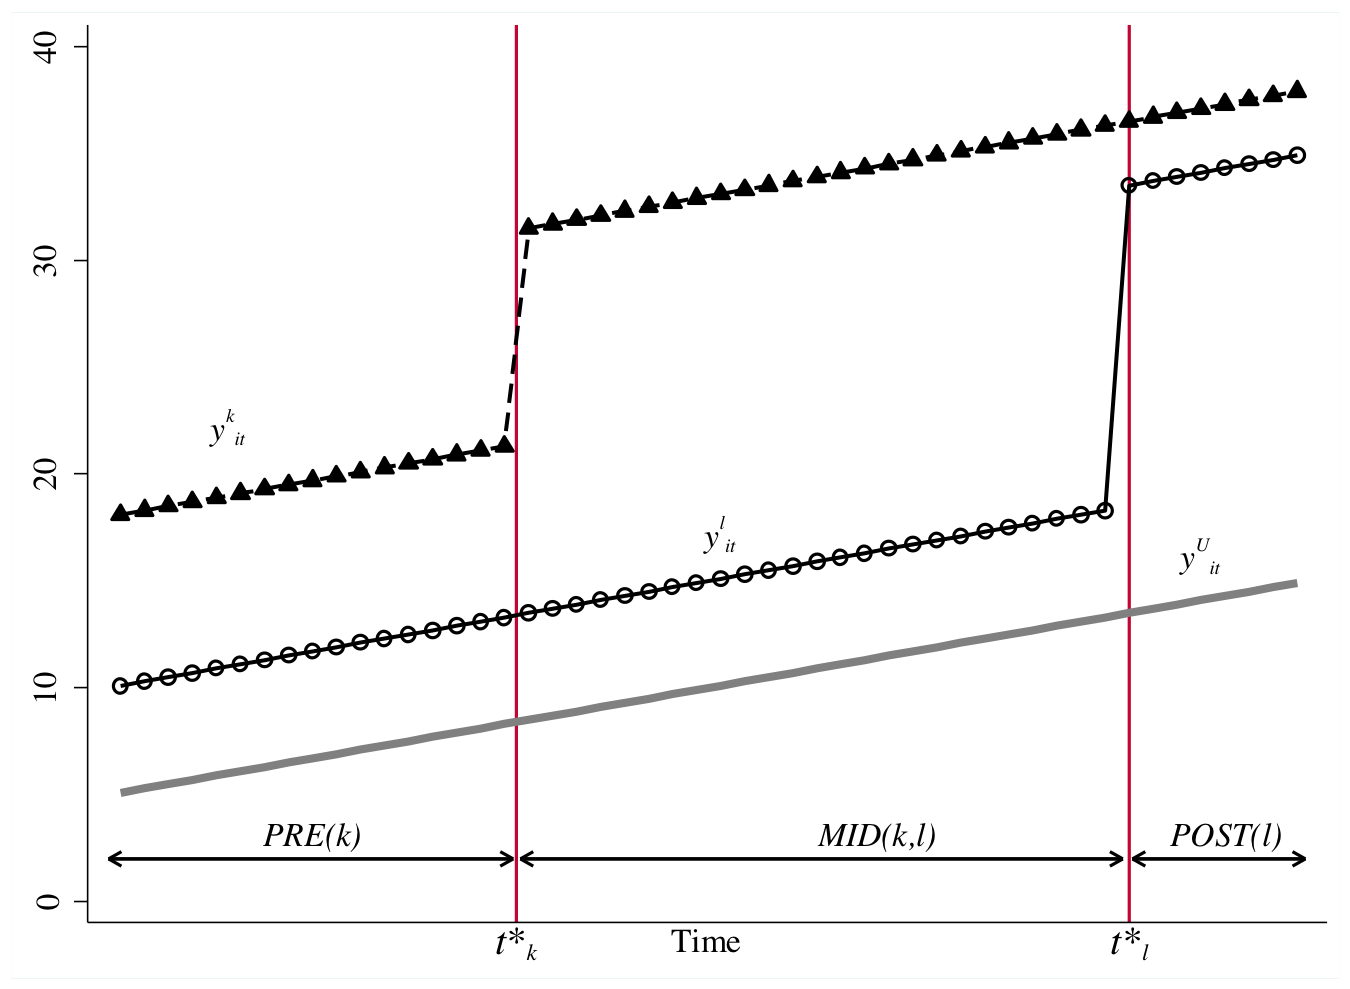
\includegraphics[height=0.70\textheight,keepaspectratio]{figures/bacon_goodman_2.png}
\end{center}
\vspace{-0.3em}
\meta{Three groups: $k$ treated early ($t^*_k$), $l$ treated late ($t^*_l$), $U$ never treated. \;Bacon (2021): staggered TWFE is a weighted sum of \textbf{four} 2$\times$2s built from these windows.}
\end{frame}

%% ---------- Slide 38d2: Clean 2x2 — Early vs Untreated ----------
\begin{frame}{Clean 2$\times$2 \#1: Early vs Untreated}
\vspace{-0.4em}
\begin{center}
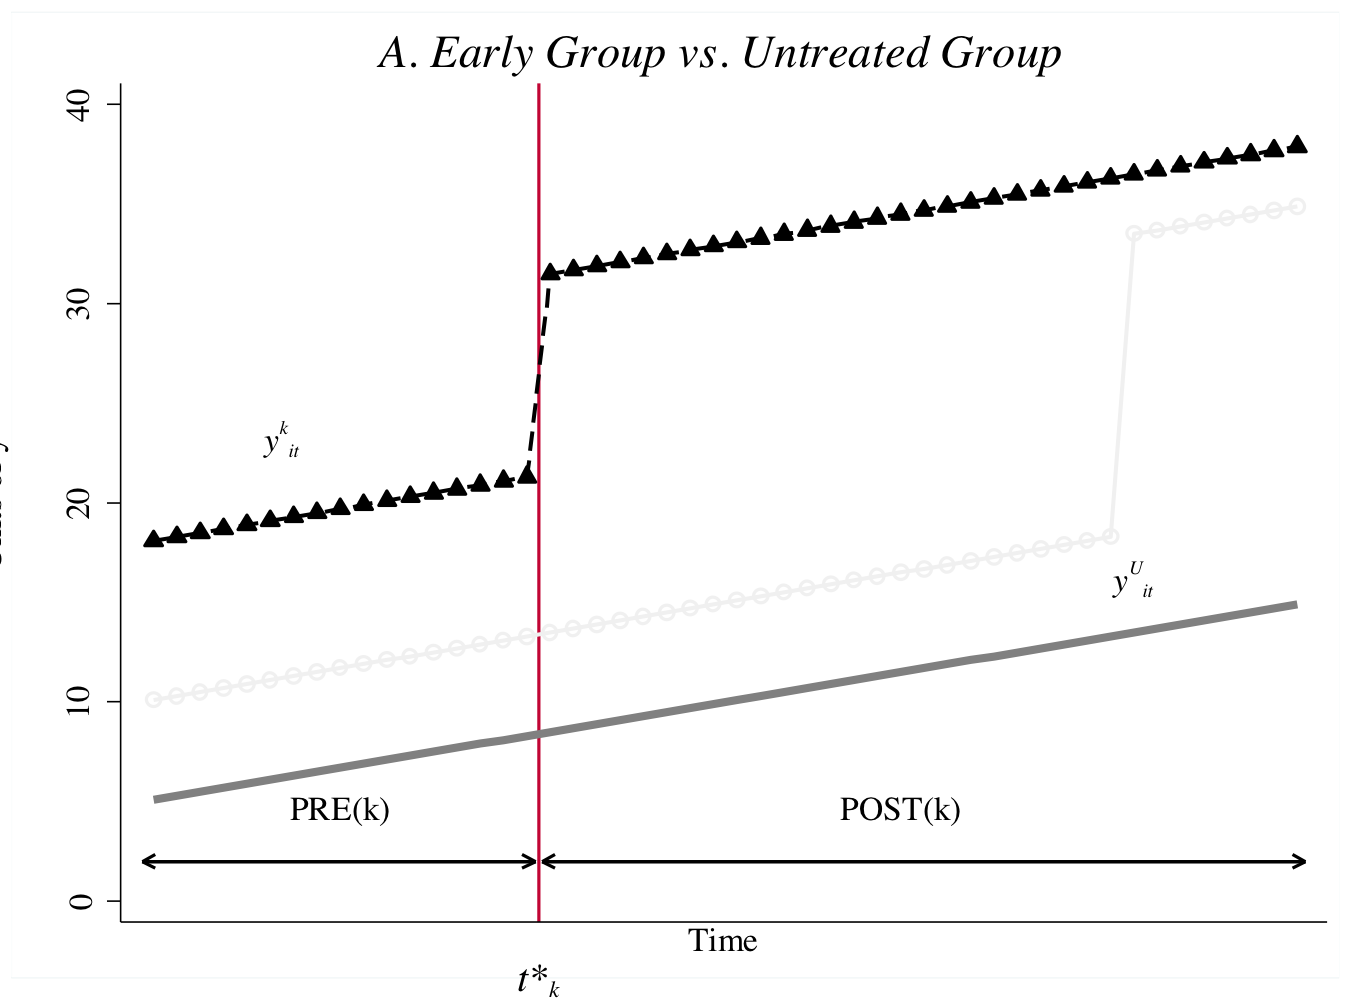
\includegraphics[height=0.70\textheight,keepaspectratio]{figures/bacon_goodman_3.png}
\end{center}
\vspace{-0.3em}
\meta{Pre $=$ before $t^*_k$, Post $=$ after $t^*_k$. \;$U$ never receives treatment, so its observed $Y$ is always $Y(0)$. \;\highlight{Identifies ATT$(k)$} under PT.}
\end{frame}

%% ---------- Slide 38d3: Clean 2x2 — Late vs Untreated ----------
\begin{frame}{Clean 2$\times$2 \#2: Late vs Untreated}
\vspace{-0.4em}
\begin{center}
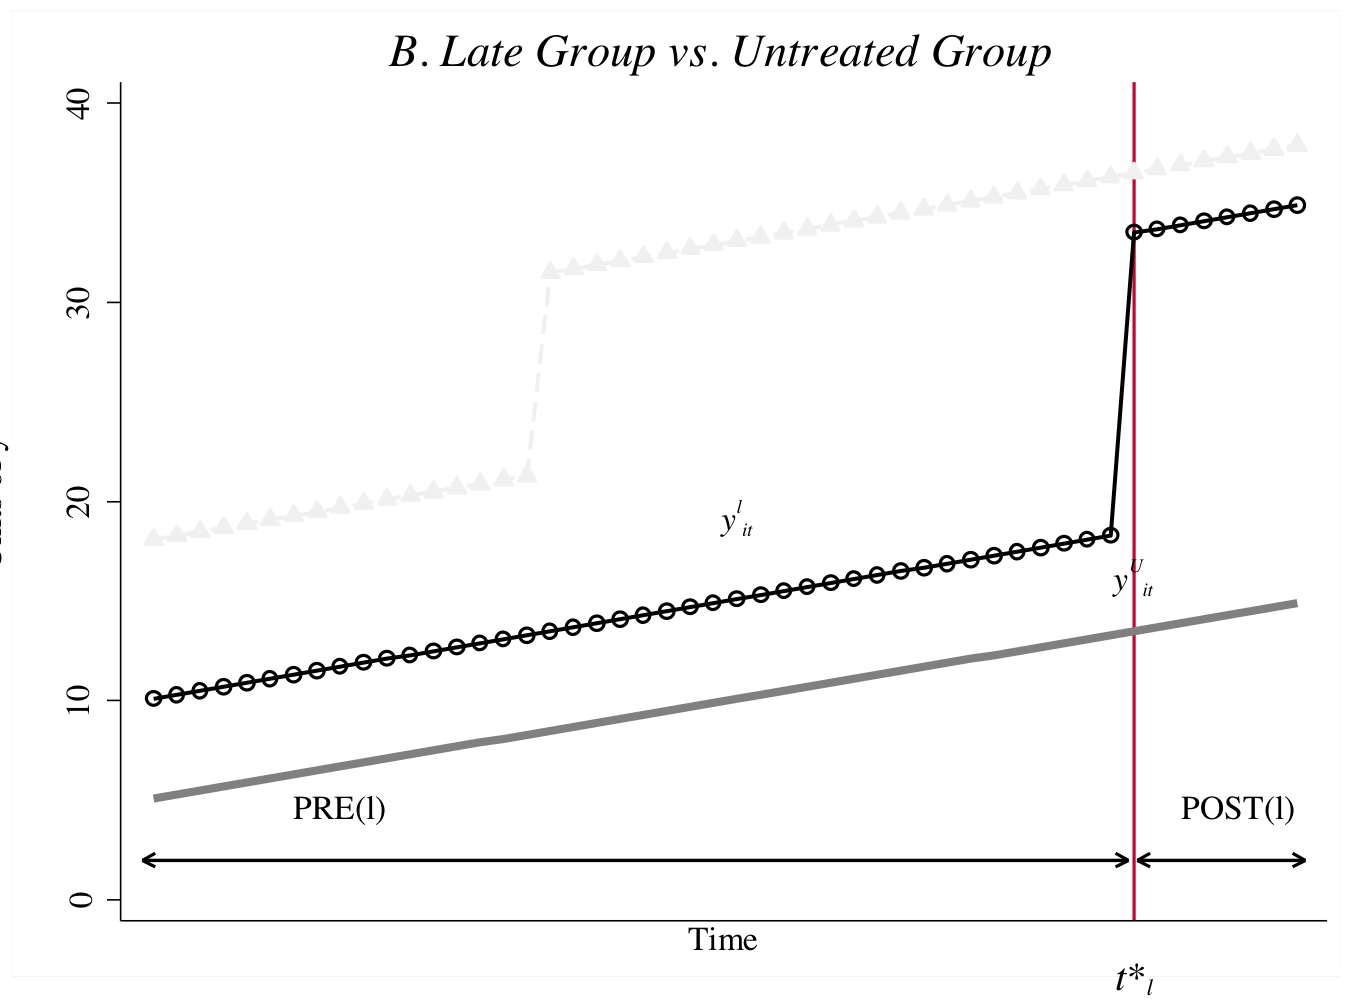
\includegraphics[height=0.70\textheight,keepaspectratio]{figures/bacon_goodman_4.png}
\end{center}
\vspace{-0.3em}
\meta{Pre $=$ before $t^*_l$, Post $=$ after $t^*_l$. \;Same logic: $U$ stays $Y(0)$ throughout. \;\highlight{Identifies ATT$(l)$} under PT.}
\end{frame}

%% ---------- Slide 38d4: Clean 2x2 — Early vs Late (not-yet-treated control) ----------
\begin{frame}{Clean 2$\times$2 \#3: Early vs Late \meta{\textmd{(Late is not-yet-treated)}}}
\vspace{-0.4em}
\begin{center}
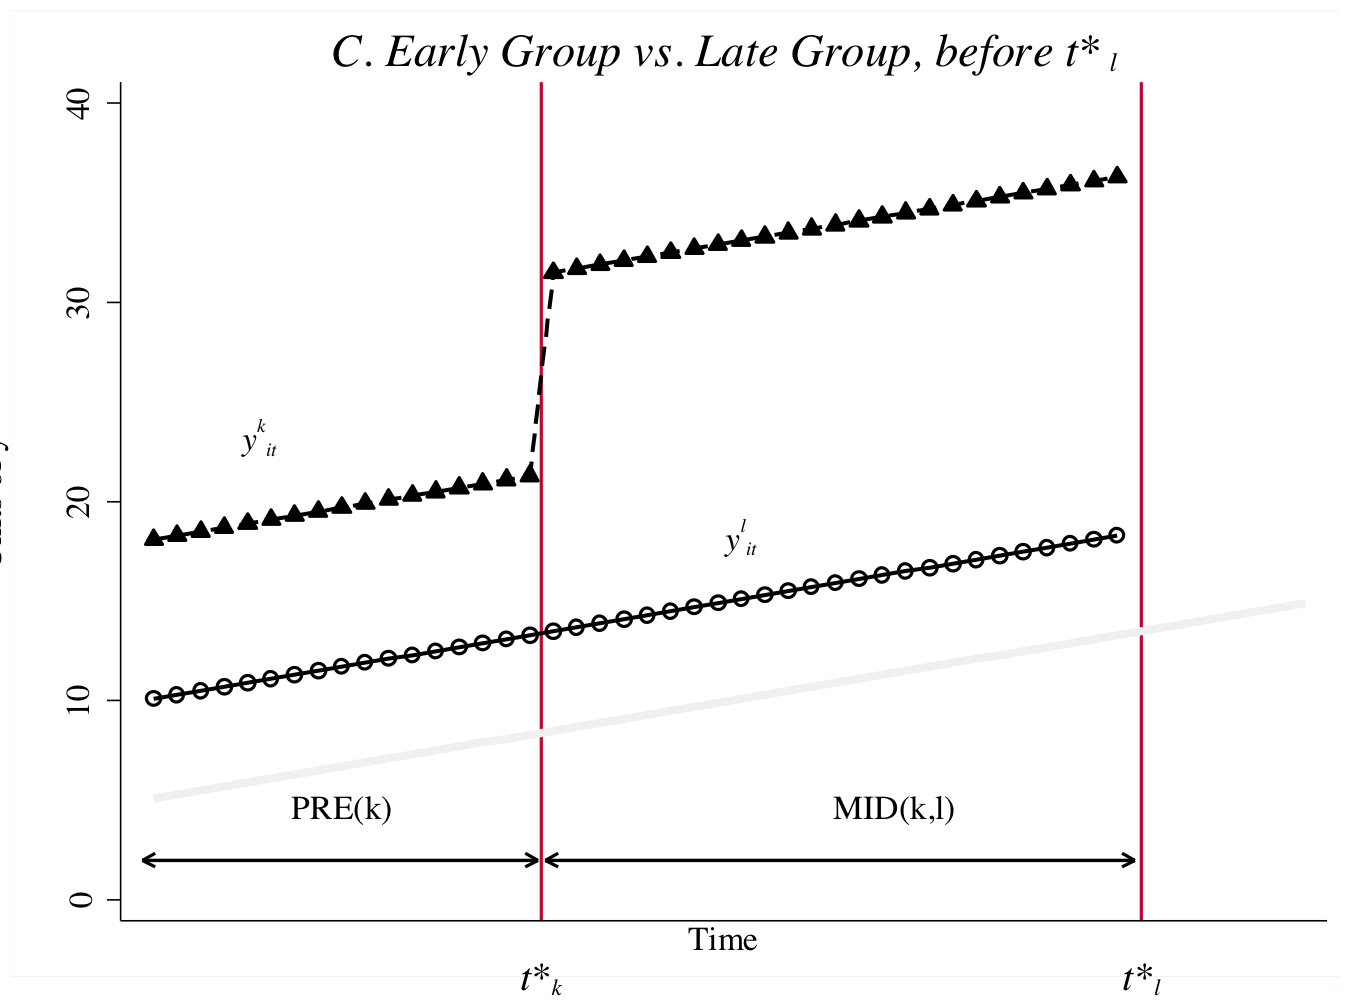
\includegraphics[height=0.68\textheight,keepaspectratio]{figures/bacon_goodman_6.png}
\end{center}
\vspace{-0.3em}
\meta{Window: $\text{PRE}(k)$ vs $\text{MID}(k,l)$. \;$l$ is valid \textit{here} because it hasn't been treated yet ($Y^l = Y(0)$). \;\highlight{Identifies ATT$(k)$ over MID} under PT. \;Modern estimators (CS, dCdH, SA) preserve this move.}
\end{frame}

%% ---------- Slide 38d5: Forbidden 2x2 — Late vs Early (already-treated control) ----------
\begin{frame}{Forbidden 2$\times$2: Late vs Early \meta{\textmd{(Early is already-treated)}}}
\vspace{-0.4em}
\begin{center}
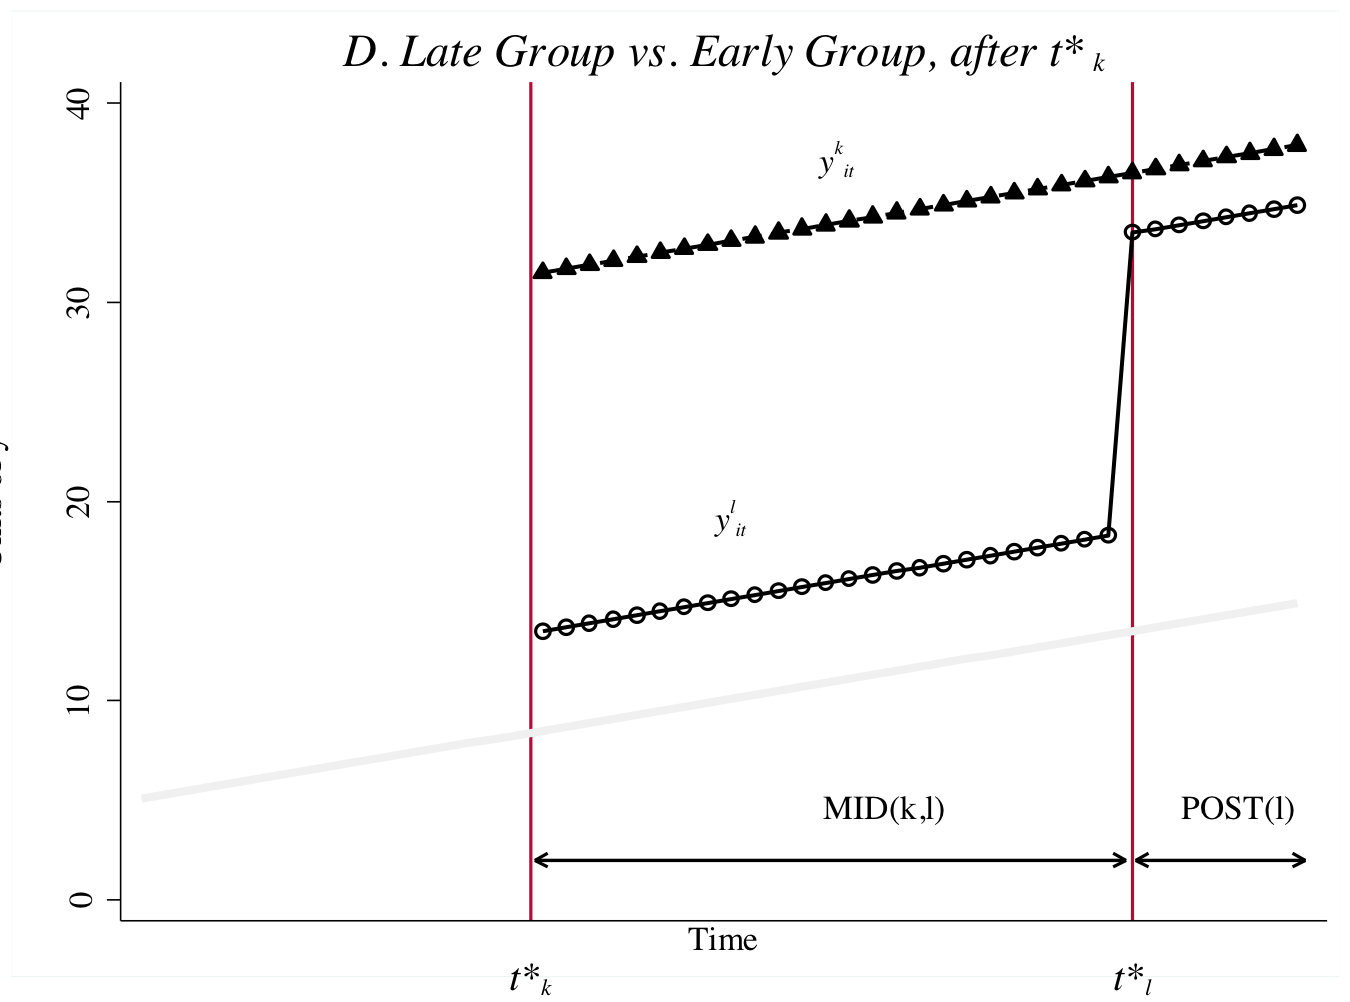
\includegraphics[height=0.62\textheight,keepaspectratio]{figures/bacon_goodman_7.png}
\end{center}
\vspace{-0.3em}
\meta{Window: $\text{MID}(k,l)$ vs $\text{POST}(l)$. \;The ``control'' is $k$ --- \textbf{already-treated}, with effects that move. \;Bias $=-\Delta\text{ATT}_k$. \;\highlight{This is Case 4 from the simulation, in disguise.} \;TWFE silently aggregates this with the three clean 2$\times$2s above.}
\end{frame}

%% ---------- Slide 38c: No Anticipation — the "trivial" assumption ----------
\begin{frame}{No Anticipation --- the other assumption}
\footnotesize
Step 2 of the proof used $Y_{\text{Pre}} = Y(0)$ for the treated group. That step has a name: \highlight{No Anticipation (NA).}
\begin{block}{What NA says}
For any unit, $Y_t = Y_t(0)$ at every $t$ before its treatment date. \;Units don't respond to a treatment they haven't received yet.
\end{block}
\textbf{Holds trivially if \textit{either}:}
\begin{enumerate}
  \item \textbf{Treatment effects are zero in the pre-period} --- if a unit hasn't been treated, by construction $Y = Y(0)$.
  \item \textbf{Treatment is unanticipated} --- agents don't see it coming, so they can't react ahead of time.
\end{enumerate}
\textbf{Examples.}
\begin{itemize}
  \item \textit{NA holds:} a state will let you drive without a license next year. You can't today. $Y = Y(0)$. \checkmark
  \item \textit{NA fails:} you'll win the lottery tomorrow and you know it. You buy a house today. $Y \neq Y(0)$. $\times$
\end{itemize}
\end{frame}

%% ---------- Slide 38d: The cost of losing NA ----------
\begin{frame}{The cost of losing No Anticipation}
\footnotesize
If the pre-period is contaminated by anticipation, $Y_{\text{Pre}}$ for the treated group is $Y(1)$, not $Y(0)$. The 2$\times$2 now identifies:
\vspace{-0.3em}
\[
\widehat{\text{DiD}} \;=\; \underbrace{\text{ATT}_{\text{Post}}}_{\text{what we want}} \;+\; \underbrace{\text{non-PT bias}}_{\text{still there}} \;-\; \underbrace{\textcolor{accent}{\text{ATT}_{\text{Pre}}}}_{\text{the anticipation effect}}
\]
\vspace{-0.4em}
\begin{itemize}
  \item If treatment effects are roughly constant over time, DiD can collapse to \highlight{zero} despite a real effect.
  \item Sign and magnitude of the bias depend on \textit{when} you set the baseline.
\end{itemize}
\vspace{0.2em}
\begin{block}{The fix: roll the baseline back}
Push the pre-period earlier --- before any anticipation could plausibly have started. Clean $Y(0)$ baseline. \\
\highlight{Side effect:} PT now has to hold over the longer window. ATT is still identified.
\end{block}
\end{frame}

%% ---------- Slide 39: PT is weaker than randomization ----------
\begin{frame}{Parallel trends is weaker than randomization}
\vspace{0.2em}
\begin{center}
\begin{tikzpicture}[scale=1.0]
%% Axes (extended to give labels room on the right)
\draw[->, slate, thick] (0,0) -- (6.8,0) node[right, text=charcoal, font=\small] {time};
\draw[->, slate, thick] (0,0) -- (0,3.3) node[above, text=charcoal, font=\small] {$Y$};

%% Treatment-time vertical reference
\draw[dashed, warmgray] (2.5,0) -- (2.5,3.1);
\node[font=\scriptsize, text=warmgray, anchor=north] at (2.5,-0.1) {treatment};

%% Control: Y(0) for D=0 — slope 0.2 throughout. Ends at x=4.5.
\draw[trendcontrol] (0.3,0.6) -- (4.5,1.44);

%% Treated PRE: Y(0) for D=1 — same slope as control (parallel)
\draw[trendline] (0.3,1.6) -- (2.5,2.04);

%% Treated POST observed: diverges upward (slope 0.4)
\draw[trendline] (2.5,2.04) -- (4.5,2.84);

%% Counterfactual: Y(0) for D=1 — parallel to control (slope 0.2)
\draw[line width=0.8pt, accent, densely dotted] (2.5,2.04) -- (4.5,2.44);

%% ATT bracket — placed OUTSIDE the data region (x=4.7) so no line crosses it
\draw[<->, accent, line width=0.5pt] (4.7,2.44) -- (4.7,2.84);
\node[font=\scriptsize, text=accent, anchor=west] at (4.78,2.64) {ATT};

%% Line endpoint labels — placed further right (x=5.3) clear of bracket and ATT
\node[font=\scriptsize, text=slate,  anchor=west] at (5.3,1.44) {control $= Y(0)$};
\node[font=\scriptsize, text=accent, anchor=west] at (5.3,2.84) {treated $= Y(1)$};
\node[font=\scriptsize, text=accent, anchor=west] at (5.3,2.44) {$Y(0)$ counter.};

\end{tikzpicture}
\end{center}
\vspace{0.2em}
\begin{center}
\small\color{warmgray}\itshape
All three $Y(0)$ trajectories (control, treated-pre, counterfactual) share one slope. \\ Levels can differ. Trends must move together.
\end{center}
\end{frame}

%% ---------- Slide 40: Both ingredients ----------
\begin{frame}{Now we have both ingredients}
\vspace{0.4em}
\begin{center}
\begin{tikzpicture}
\node[ingredientdone] (calc) at (-3.2,0) {%
  \textcolor{accent}{\large 1. \checkmark} \\[0.3em]
  A \textit{calculation}\\[0.2em]
  \scriptsize\textcolor{warmgray}{(the 2$\times$2)}
};
\node[ingredientdone] (assn) at (3.2,0) {%
  \textcolor{accent}{\large 2. \checkmark} \\[0.3em]
  An \textit{assumption}\\[0.2em]
  \scriptsize\textcolor{warmgray}{(parallel trends)}
};
\node[font=\Large\bfseries,text=accent] at (0,0) {+};
\node[font=\large, text=charcoal, anchor=north] at (0,-1.5) {$\longrightarrow$\quad\bfseries ATT};
\end{tikzpicture}
\end{center}
\end{frame}

%% ---------- Google Sheet walkthrough (now last slide of Lesson 4) ----------
\begin{frame}{Open the sheet --- stability and trends, by hand}
\vspace{0.5em}
\begin{itemize}
  \item Four tabs in sequence: \texttt{Potential Outcomes} $\rightarrow$ \texttt{2X2} $\rightarrow$ \texttt{Balancing} $\rightarrow$ \texttt{2XT \#1}
  \item Show: $Y = Y(0)$ pre-treatment, for everyone
  \item Show: $Y = Y(0)$ for control units, \textit{regardless} of what treated units do
  \item That second point is \highlight{stability} --- one unit's treatment doesn't change another's $Y(0)$
\end{itemize}
\vspace{1em}
\meta{Sheet: \url{https://docs.google.com/spreadsheets/d/1onabpc14JdrGo6NFv0zCWo-nuWDLLV2L1qNogDT9SBw/edit}}
\end{frame}

%% =====================================================================
%%                                LESSON 5
%% =====================================================================
\remixsection{4.\ Standard Errors \\[0.3em] {\normalsize\normalfont Vanilla, Robust, Cluster-Robust}}

%% ---------- Slide A-1: DID-SPECIFIC FRAMING — Bertrand-Duflo-Mullainathan dual ----------
\begin{frame}{DiD has two kinds of bias --- not one}
\vspace{0.4em}
\pullquote{How Much Should We Trust Differences-in-Differences Estimates?}{Bertrand, Duflo \& Mullainathan, \textit{QJE} 2004}
\vspace{0.4em}
\begin{block}{Two distinct failure modes}
\small
\textbf{(1) Biased estimator.} Non-parallel trends contaminate $\hat\beta$ --- covered in Lessons 1--3. \\[0.2em]
\textbf{(2) Biased inference.} Even with $\hat\beta$ unbiased, a wrong SE gives the wrong $t$, $p$, and CI.
\end{block}
\vspace{0.3em}
\begin{itemize}\small
  \item Heteroskedasticity and within-cluster correlation are \textit{inference} problems, not identification problems.
  \item BDM's alarm bell: DiD with vanilla SE rejects a true null at $\approx 45\%$ instead of $5\%$.
  \item This lesson: \highlight{get the spread right} so the test you reported is the test you actually ran.
\end{itemize}
\end{frame}

%% ---------- Slide A0: THE STAKES — over-rejection ----------
\begin{frame}{The stakes: a wrong standard error is a false positive}
\vspace{0.4em}
We design hypothesis tests to control the false-positive rate:
\vspace{-0.1em}
\[
\text{size} \;=\; \Pr(\text{reject } H_0 \mid H_0 \text{ is true}) \;\stackrel{!}{=}\; \alpha \;\;(\text{typically } 5\%).
\]
\vspace{-0.4em}
\begin{itemize}\small
  \item Get the SE right $\Rightarrow$ you reject a true null $\approx 5\%$ of the time. As advertised.
  \item Get the SE \textit{too small} $\Rightarrow$ $|t|$ inflated $\Rightarrow$ you reject at $\mathbf{10\%}$, $\mathbf{20\%}$, sometimes $\mathbf{45\%}$. \\
        You publish ``significant'' results that are noise.
\end{itemize}
\vspace{0.4em}
\begin{block}{The whole point of this lesson}
\small
The OLS point estimate $\hat\beta$ is \textit{fine} --- unbiased for the ATT \textbf{under parallel trends}. \\
\highlight{What we're fixing is the spread we report around it.} \;Same data, same $\hat\beta$ --- different inference.
\end{block}
\end{frame}

%% ---------- Slide A1: visual of size distortion ----------
\begin{frame}{Same $\hat\beta$, two reported spreads, two test sizes}
\vspace{0.3em}
\begin{center}
\begin{tikzpicture}[scale=0.85]
  %% True beta marker
  \draw[charcoal, very thick, dashed] (5.5,-0.4) -- (5.5,4.5)
    node[above, font=\scriptsize\bfseries, text=charcoal] {true $\beta$};

  %% Correct (robust) bell + CI
  \begin{scope}[yshift=2.7cm]
    \draw[forest, thick, domain=2.8:8.2, samples=60]
      plot(\x, {1.8*exp(-0.5*((\x-5.5)/0.95)^2)});
    \draw[forest, very thick] (3.64,-0.15) -- (7.36,-0.15);
    \draw[forest, thick] (3.64,-0.30) -- (3.64,0.00);
    \draw[forest, thick] (7.36,-0.30) -- (7.36,0.00);
    \node[font=\footnotesize\bfseries, text=forest, anchor=west] at (0.0,1.5) {Correct SE};
    \node[font=\scriptsize, text=forest, anchor=west] at (0.0,1.0) {size $\approx 5\%$};
  \end{scope}

  %% Wrong (naive) bell + CI
  \begin{scope}[yshift=0.0cm]
    \draw[accent, thick, domain=3.9:7.1, samples=60]
      plot(\x, {2.2*exp(-0.5*((\x-5.5)/0.45)^2)});
    \draw[accent, very thick] (4.62,-0.15) -- (6.38,-0.15);
    \draw[accent, thick] (4.62,-0.30) -- (4.62,0.00);
    \draw[accent, thick] (6.38,-0.30) -- (6.38,0.00);
    \node[font=\footnotesize\bfseries, text=accent, anchor=west] at (0.0,1.5) {Wrong SE};
    \node[font=\scriptsize, text=accent, anchor=west] at (0.0,1.0) {size $\gg 5\%$};
  \end{scope}
\end{tikzpicture}
\end{center}
\vspace{0.1em}
\begin{center}
\footnotesize\color{warmgray}\itshape
$\hat\beta$ is in the same place --- unbiasedness intact. The reported \textit{spread} is wrong --- and that IS the problem. \\
``You think you're running a 5\% test. You're actually running a 15\% test.''
\end{center}
\end{frame}

%% ---------- Slide A: unbiased point estimate, biased SE ----------
\begin{frame}{The point estimate can be unbiased --- the standard error often is not}
\vspace{0.6em}
\begin{itemize}
  \item OLS gives us a $\hat\beta$ that converges to the right thing under PT + NA + SUTVA
  \item But the \textit{spread} of $\hat\beta$ across hypothetical samples --- the standard error --- depends on the error structure
  \item Wrong SE $\rightarrow$ wrong $t$-statistic $\rightarrow$ wrong $p$-value $\rightarrow$ wrong conclusion
\end{itemize}
\vspace{0.6em}
\meta{Two problems: heteroskedasticity, and within-cluster (= serial) correlation.}
\end{frame}

%% ---------- Slide A2: WHAT AN SE ACTUALLY IS ----------
\begin{frame}{What an SE \textit{is}: the variance of $\hat\beta$ across hypothetical samples}
\vspace{0.4em}
\begin{itemize}\small
  \item $\hat\beta$ is a \textbf{random variable}. Different samples from the same DGP give different $\hat\beta$'s.
  \item The \highlight{sampling distribution} of $\hat\beta$ is the distribution we'd see if we re-drew the sample many times.
  \item The \highlight{standard error} is the standard deviation of that distribution: \;$\text{SE}(\hat\beta) = \sqrt{\text{Var}(\hat\beta)}$.
\end{itemize}
\vspace{0.4em}
\begin{block}{The weird part}
\small
We only ever see \textit{one sample}. But we're trying to describe how $\hat\beta$ would \textit{vary} across samples we never drew. \\
\highlight{The SE formula is what lets us estimate the across-sample variance from a single sample.} The rest of this lesson is about whether we did that right.
\end{block}
\end{frame}

%% ---------- Slide B: three flavors ----------
\begin{frame}{Three flavors of standard error}
\vspace{0.6em}
\begin{itemize}
  \item \highlight{Vanilla (homoskedastic)}: assumes $\text{Var}(\varepsilon_i \mid X_i) = \sigma^2$ for all $i$
  \item \highlight{Robust (Eicker-Huber-White)}: lets each residual speak for itself --- handles heteroskedasticity
  \item \highlight{Cluster-robust (CRVE)}: groups residuals by cluster, lets within-cluster errors correlate freely
\end{itemize}
\vspace{0.6em}
\meta{Same point estimate, three different SEs. The SE you pick is a claim about the error structure.}
\end{frame}

%% ---------- Slide B2: THE GENERAL FORMULA — the sandwich named ----------
\begin{frame}{The general formula: a ``sandwich''}
\vspace{0.4em}
The variance of $\hat\beta$ across hypothetical samples has one general form:
\vspace{-0.2em}
\[
\text{Var}(\hat\beta) \;=\; \underbrace{(X'X)^{-1}}_{\textstyle \text{bread}}\;\; \underbrace{X'\,\text{Var}(\varepsilon \mid X)\,X}_{\textstyle \text{meat}} \;\; \underbrace{(X'X)^{-1}}_{\textstyle \text{bread}}.
\]
\vspace{0.0em}
\begin{itemize}\small
  \item The \textbf{bread} $(X'X)^{-1}$ comes from OLS mechanics. We always have it.
  \item The \textbf{meat} $X' \text{Var}(\varepsilon \mid X)\, X$ is where the \textit{error structure} lives.
  \item All three flavors (vanilla, robust, cluster-robust) have the same bread. \\ \highlight{They differ only in how they estimate the meat.}
\end{itemize}
\vspace{0.4em}
\begin{center}
\small\color{warmgray}\itshape
The rest of this lesson: what goes in the middle, and what changes if we get it wrong.
\end{center}
\end{frame}

%% ---------- Slide C0: HOMOSKEDASTICITY — the collapse ----------
\begin{frame}{Homoskedasticity: the sandwich collapses}
\vspace{0.3em}
\textbf{Assumption.}\;\; $\text{Var}(\varepsilon_i \mid X_i) = \sigma^2$ \;(constant, doesn't depend on $X_i$).
\vspace{0.5em}

Start from the general sandwich:
\vspace{-0.2em}
\[
\text{Var}(\hat\beta) \;=\; (X'X)^{-1}\, \big(X' \,\text{Var}(\varepsilon \mid X)\, X\big)\, (X'X)^{-1}
\]
\vspace{-0.2em}

Under homoskedasticity $\text{Var}(\varepsilon \mid X) = \sigma^2 \mathbf{I}$, so $X'\sigma^2\mathbf{I}\,X = \sigma^2 (X'X)$, and the sandwich collapses:
\vspace{-0.2em}
\[
\text{Var}(\hat\beta) \;=\; (X'X)^{-1}\, \sigma^2(X'X)\, (X'X)^{-1} \;=\; \sigma^2 (X'X)^{-1}.
\]
\vspace{0.1em}
\begin{itemize}\small
  \item One scalar $\widehat\sigma^2 = \tfrac{1}{n-k}\sum_i \hat e_i^2$ summarizes \textit{all} the noise.
  \item This is what \texttt{lm()} reports by default. \highlight{Clean --- only if homoskedasticity holds.}
\end{itemize}
\end{frame}

%% ---------- Slide C: HETEROSKEDASTICITY — the collapse breaks ----------
\begin{frame}{Heteroskedasticity: the collapse breaks}
\vspace{0.5em}
Now $\sigma_i^2 = \text{Var}(\varepsilon_i \mid X_i)$ varies with $i$. The middle of the sandwich is:
\vspace{-0.2em}
\[
X'\, \text{diag}(\sigma_1^2, \,\sigma_2^2, \,\dots,\, \sigma_n^2)\, X \;\;\neq\;\; \sigma^2 (X'X).
\]
\vspace{-0.2em}
\begin{itemize}\small
  \item Each $\sigma_i^2$ on the diagonal is the variance of $Y_i$ given $X_i$ --- the noise around the regression line for that observation.
  \item In a DiD with binary $D$, that means: treated observations have one variance, controls have another.
  \item No single $\sigma^2$ can scale this matrix out. \highlight{The collapse fails.}
\end{itemize}
\vspace{0.3em}
\begin{center}
\small\color{warmgray}\itshape Next: the Eicker--Huber--White fix.
\end{center}
\end{frame}

%% ---------- Slide C-a: EHW fix — the sandwich estimator ----------
\begin{frame}{Eicker--Huber--White: let each residual speak for itself}
\vspace{0.4em}
We don't know $\sigma_i^2$. Replace it with the empirical $\hat e_i^2$. The sandwich stays a sandwich:
\vspace{-0.2em}
\[
\widehat{\text{Var}}_{\text{HC}}(\hat\beta) \;=\; (X'X)^{-1}\, \bigg(\sum_i \hat e_i^2\, X_i X_i'\bigg)\, (X'X)^{-1}.
\]
\vspace{0.1em}
\begin{itemize}\small
  \item Each $\hat e_i^2$ enters \textit{weighted} by that observation's leverage $X_iX_i'$.
  \item No assumption of constant variance. Each obs's noise speaks for itself.
\end{itemize}
\vspace{0.3em}
\begin{block}{The HC family --- four small-sample corrections}
\footnotesize
\textbf{HC0} (raw): the formula above, exactly. \;
\textbf{HC1}: multiply by $n/(n-k)$ to correct for the degrees of freedom used fitting $\hat\beta$. Stata's default. \\
\textbf{HC2 / HC3}: also divide each $\hat e_i^2$ by $(1-h_{ii})$ or $(1-h_{ii})^2$ to penalize high-leverage observations. \\
\highlight{HC1 is what we'll use below.}
\end{block}
\end{frame}

%% ---------- Slide C2: HC1 numerical worked example ----------
\begin{frame}[shrink=8]{HC1 numerically: each $\hat e_i^2$ weighted by leverage}
\vspace{0.2em}
\textbf{Six observations.}\; Three pairs at $\tilde x \in \{-2, 0, +2\}$.\; Fitted $\hat\beta_1 = 1$; residuals shown.
\vspace{0.5em}
\begin{center}
\renewcommand{\arraystretch}{1.15}
\footnotesize
\begin{tabular}{@{}cccrrr@{}}
\toprule
$i$ & cluster $g$ & $\tilde x_i$ & $\hat e_i$ & $\hat e_i^2$ & $\tilde x_i^2 \cdot \hat e_i^2$ \\
\midrule
1 & \textcolor{accent}{1} & $-2$ & $+0.5$ & $0.25$ & \textcolor{accent}{$1.00$} \\
2 & \textcolor{accent}{1} & $-2$ & $+0.5$ & $0.25$ & \textcolor{accent}{$1.00$} \\
3 & \textcolor{ocean}{2}  & $0$  & $-1.0$ & $1.00$ & $0.00$ \\
4 & \textcolor{ocean}{2}  & $0$  & $-1.0$ & $1.00$ & $0.00$ \\
5 & \textcolor{forest}{3} & $+2$ & $+0.5$ & $0.25$ & \textcolor{forest}{$1.00$} \\
6 & \textcolor{forest}{3} & $+2$ & $+0.5$ & $0.25$ & \textcolor{forest}{$1.00$} \\
\midrule
\multicolumn{5}{r}{meat $\;=\;$} & $\mathbf{4.00}$ \\
\bottomrule
\end{tabular}
\end{center}
\vspace{0.4em}

With $n=6$, $k=2$, and $S_{xx} = \sum_i \tilde x_i^2 = (-2)^2{+}(-2)^2{+}0{+}0{+}2^2{+}2^2 = 16$:
\[
\widehat{\text{Var}}_{\text{HC1}}(\hat\beta_1) \;=\; \frac{n}{n-k}\cdot \underbrace{\frac{1}{S_{xx}}}_{\textstyle\text{bread}}\cdot \underbrace{\text{meat}}_{\textstyle 4.00} \cdot \underbrace{\frac{1}{S_{xx}}}_{\textstyle\text{bread}} \;=\; \frac{6}{4}\cdot \frac{4.00}{16 \cdot 16} \;=\; \frac{6}{4}\cdot \frac{4.00}{256} \;=\; 0.02344
\]
\vspace{-0.4em}
\[
\;\;\Rightarrow\;\; \highlight{$\text{SE}_{\text{HC1}} = \sqrt{0.02344} \approx 0.153$}
\]
\vspace{0.0em}
\meta{Obs 3--4 contribute zero because $\tilde x = 0$ kills the leverage weight. \;\textbf{HC1 treats all 6 obs as independent.} \\ Scalar form shown gives $\text{SE}(\hat\beta_1)$ only (intercept absorbed via FWL). The matrix sandwich returns \textit{every} coefficient's SE in one shot.}
\end{frame}

%% ---------- Slide C2b: VISUAL — sampling distribution comparison ----------
\begin{frame}{When does HC matter? Compare each SE formula to the truth.}
\vspace{0.0em}
\begin{center}
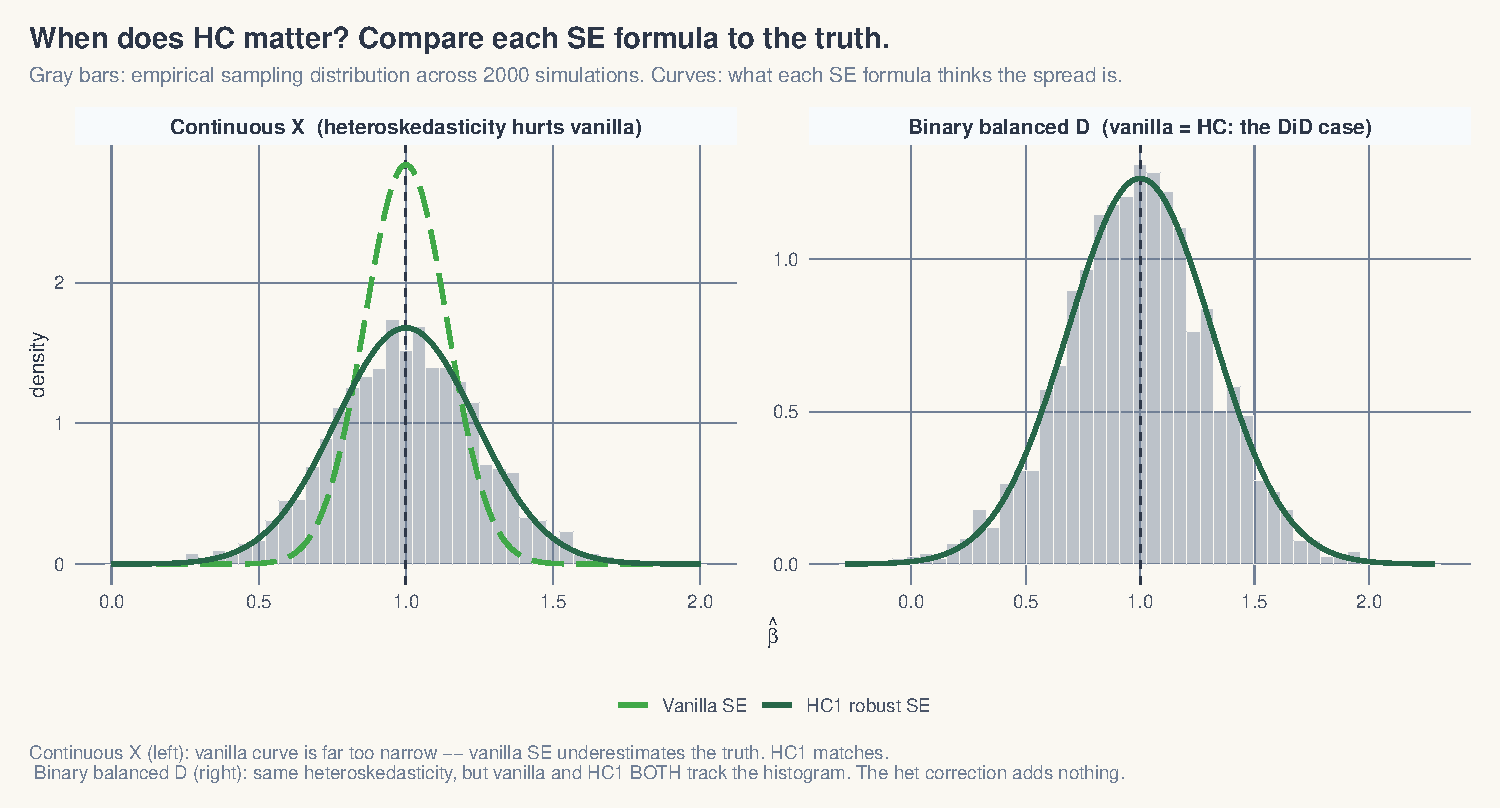
\includegraphics[width=0.96\linewidth,height=0.66\textheight,keepaspectratio]{figures/he_vs_homo.pdf}
\end{center}
\vspace{-0.3em}
\begin{center}
\footnotesize\color{warmgray}\itshape
Histogram = the true sampling distribution of $\hat\beta$ (2000 simulations). Curves = what each SE formula thinks. \\
\highlight{Continuous X:} vanilla curve is too narrow --- vanilla underestimates SD by 44\%; HC1 matches. \;
\highlight{Binary balanced D:} vanilla and HC1 \textit{both} match the histogram. The het correction adds nothing.
\end{center}
\end{frame}

%% ---------- Slide C3: Why HC barely helps in DiD ----------
\begin{frame}{Why HC-robust barely helps in DiD}
\vspace{0.4em}
The HC correction reweights residuals by $X_i X_i'$. In a DiD with binary treatment $D_i \in \{0,1\}$ and roughly balanced groups:
\vspace{0.5em}
\begin{itemize}
  \item Treated and control units have similar \textit{leverage}: each side carries $\approx$ half the weight in $X'X$.
  \item Residual variance is roughly \textit{symmetric} across the two groups (binary $D$ doesn't generate a fan shape in $\hat e^2$).
  \item So the weighted sum $\sum_i \hat e_i^2 X_i X_i'$ ends up not very different from the unweighted $\hat\sigma^2 (X'X)$.
\end{itemize}
\vspace{0.5em}
\begin{block}{Consequence}
\small
$\text{SE}_{\text{HC}} \approx \text{SE}_{\text{vanilla}}$ \;\;for typical DiD specifications. \\
\highlight{The over-rejection problem is not heteroskedasticity. It's something else.}
\end{block}
\end{frame}

%% ---------- Slide D: Bertrand Duflo Mullainathan ----------
\begin{frame}{Bertrand, Duflo \& Mullainathan (QJE 2004) --- the placebo-law test}
\vspace{0.4em}
\textbf{``How Much Should We Trust Differences-in-Differences Estimates?''}
\vspace{0.5em}
\begin{itemize}\small
  \item BDM generate \textit{placebo laws}: assign random treatment dates to states in a real CPS panel.
  \item True effect by construction: $\beta = 0$. So $\Pr(\text{reject } H_0)$ should equal $\alpha = 5\%$.
  \item \textbf{Vanilla SE}: rejection rate $\approx \mathbf{45\%}$. Wildly over-rejects.
  \item \textbf{Heteroskedasticity-robust (HC1)}: rejection rate \textit{also} $\approx 45\%$. \highlight{HC barely moves the needle.}
  \item \textbf{Cluster-robust at state level}: rejection rate $\approx \mathbf{5\%}$. The fix.
\end{itemize}
\vspace{0.4em}
\begin{block}{Why HC doesn't save you in DiD}
\small
Binary, balanced $D$ + within-state serial correlation. The het-correction has nothing to do with the actual problem. \highlight{Clustering is doing all the work.}
\end{block}
\end{frame}

%% ---------- Slide E: CRVE intuition ----------
\begin{frame}{Cluster-robust SE: sum scores within cluster, \textit{then} square}
\vspace{0.5em}
For each cluster $g$, the ``score'' is $s_g = \sum_{i \in g} \tilde x_i \hat e_i$.
\vspace{0.4em}
\[
\widehat{\text{Var}}_{\text{CRVE}}(\hat\beta) \;\propto\; (X'X)^{-1}\!\left(\sum_g s_g s_g'\right)\!(X'X)^{-1}
\]
\vspace{0.2em}
\begin{itemize}
  \item HC1 squares each \textit{observation's} contribution, then sums.
  \item CRVE \textit{sums within a cluster first} --- then squares. Cross-terms between same-cluster obs get added in.
  \item If errors are correlated within a cluster, those cross-terms are positive and the SE grows.
\end{itemize}
\end{frame}

%% ---------- Slide E2: CRVE numerical worked example (same 6 obs) ----------
\begin{frame}[shrink=10]{CRVE numerically: same 6 obs, group scores, then square}
\vspace{0.2em}
\textbf{Same 6 observations.} Now compute $s_g = \sum_{i \in g} \tilde x_i \hat e_i$ for each cluster, then $s_g^2$:
\vspace{0.4em}
\begin{center}
\renewcommand{\arraystretch}{1.15}
\footnotesize
\begin{tabular}{@{}cccrr@{}}
\toprule
$i$ & $g$ & $\tilde x_i$ & $\hat e_i$ & $\tilde x_i \hat e_i$ \\
\midrule
1 & \textcolor{accent}{1} & $-2$ & $+0.5$ & \textcolor{accent}{$-1$} \\
2 & \textcolor{accent}{1} & $-2$ & $+0.5$ & \textcolor{accent}{$-1$} \\
3 & \textcolor{ocean}{2}  & $0$  & $-1.0$ & $0$ \\
4 & \textcolor{ocean}{2}  & $0$  & $-1.0$ & $0$ \\
5 & \textcolor{forest}{3} & $+2$ & $+0.5$ & \textcolor{forest}{$+1$} \\
6 & \textcolor{forest}{3} & $+2$ & $+0.5$ & \textcolor{forest}{$+1$} \\
\bottomrule
\end{tabular}
\hspace{1.0em}
\begin{tabular}{@{}crr@{}}
\toprule
$g$ & $s_g$ & $s_g^2$ \\
\midrule
\textcolor{accent}{1}  & \textcolor{accent}{$-2$}  & \textcolor{accent}{$4$} \\
\textcolor{ocean}{2}   & $0$  & $0$ \\
\textcolor{forest}{3}  & \textcolor{forest}{$+2$} & \textcolor{forest}{$4$} \\
\midrule
\multicolumn{2}{r}{meat $=$} & $\mathbf{8}$ \\
\bottomrule
\end{tabular}
\end{center}
\vspace{0.4em}

With $G=3$, $n=6$, $k=2$, and $S_{xx} = \sum_i \tilde x_i^2 = (-2)^2{+}(-2)^2{+}0{+}0{+}2^2{+}2^2 = 16$, so $S_{xx}^2 = 256$:
\[
\widehat{\text{Var}}_{\text{CRVE}}(\hat\beta_1) \;=\; \tfrac{G}{G-1}\cdot \tfrac{n-1}{n-k}\cdot \tfrac{\text{meat}}{S_{xx}^2} \;=\; \tfrac{3}{2}\cdot \tfrac{5}{4}\cdot \tfrac{8}{256} \;=\; 0.05859
\;\;\Rightarrow\;\; \highlight{$\text{SE}_{\text{CRVE}} \approx 0.242$}
\]
\begin{center}
\small\color{warmgray}\itshape
\textbf{HC1}: 0.153 \quad vs.\quad \textbf{CRVE}: 0.242 \quad (\highlight{58\% larger}). \;Same data. The cluster cross-terms changed the meat from 4 to 8.
\end{center}
\end{frame}

%% ---------- Slide E3: side-by-side formulas ----------
\begin{frame}{Two formulas side by side}
\vspace{0.4em}
\begin{center}
\renewcommand{\arraystretch}{1.5}
\footnotesize
\begin{tabular}{@{}c | c@{}}
\textbf{HC1 (obs independent)} & \textbf{CRVE (cluster-robust)} \\[0.5em]
$\dfrac{n}{n-k}\cdot \dfrac{\sum_i \tilde x_i^2 \hat e_i^2}{\big(\sum_i \tilde x_i^2\big)^2}$
&
$\dfrac{G}{G-1}\cdot \dfrac{n-1}{n-k}\cdot \dfrac{\sum_g s_g^2}{\big(\sum_i \tilde x_i^2\big)^2}$ \\[1.4em]
sum each $\hat e_i^2 \tilde x_i^2$ separately
&
$s_g = \sum_{i \in g} \tilde x_i \hat e_i$, \;\;\text{then sum } $s_g^2$ \\
\end{tabular}
\end{center}
\vspace{0.7em}
\begin{itemize}\small
  \item HC1 sums squared per-obs contributions: cross-terms within a cluster are \textit{ignored}.
  \item CRVE sums within a cluster \textit{before} squaring: cross-terms are \textit{captured}.
  \item Matrix form: same sandwich $(X'X)^{-1}\big(\text{meat}\big)(X'X)^{-1}$, but meat differs.
\end{itemize}
\vspace{0.2em}
\meta{Same shape --- bread, meat, bread. Difference: whether the meat sums over obs or over clusters.}
\end{frame}

%% ---------- Slide G: simulation setup ----------
\begin{frame}{The simulation we'll show: 2000 placebo regressions}
\vspace{0.4em}
\begin{itemize}\small
  \item DGP: $y_{ig} = 0.4 + 0 \cdot x_{ig} + \varepsilon_{ig}$, \;\;$1000$ obs, $50$ clusters of $20$.
  \item \highlight{True $\beta_1 = 0$.} Any rejection at $\alpha=5\%$ is a false positive.
  \item Sweep three scenarios:
  \begin{itemize}\small
    \item[--] \textbf{1.} No clustering ($\rho=0$), vanilla SE
    \item[--] \textbf{2.} Clustering ($\rho=0.5$), vanilla SE
    \item[--] \textbf{3.} Clustering ($\rho=0.5$), \textit{cluster-robust} SE
  \end{itemize}
  \item For each scenario, draw 100 of the 2000 95\% CIs and color them \textbf{\color{forest}Hit} or \textbf{\color{accentdark}Missed} against the true $\beta_1 = 0$.
\end{itemize}
\vspace{0.2em}
\meta{Pattern: Yanai $\rightarrow$ Cunningham, \textit{Mixtape} \S2.27. Script: \texttt{decks/code/SE-Demo/ci\_forest\_plot.R}.}
\end{frame}

%% ---------- Slide G2: THE FOREST PLOT ----------
\begin{frame}{Coverage of 95\% CIs across the three scenarios}
\begin{center}
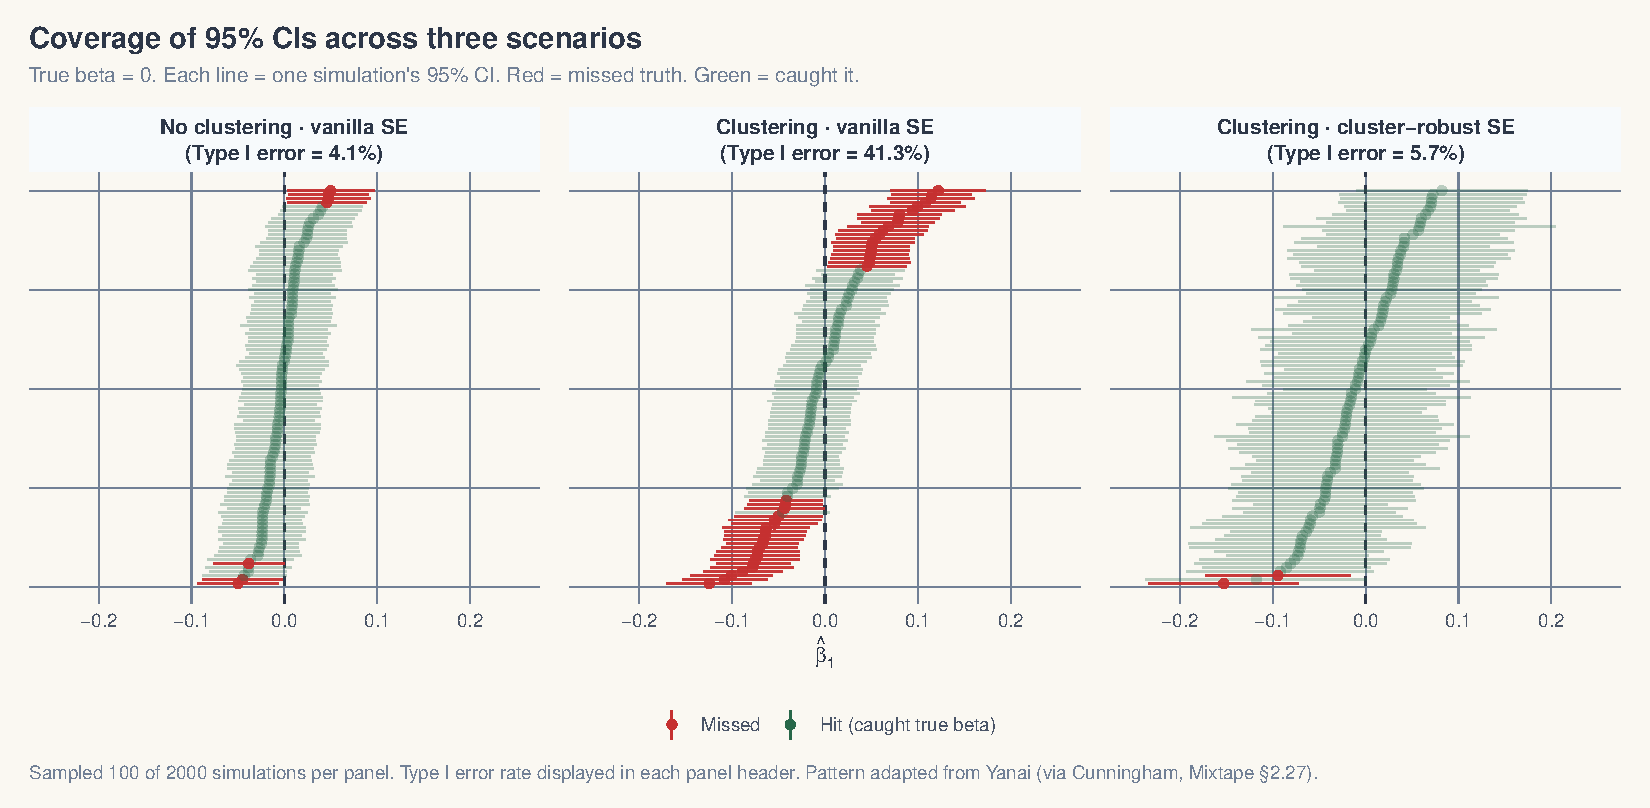
\includegraphics[width=0.98\linewidth,height=0.62\textheight,keepaspectratio]{figures/cluster_ci_forest.pdf}
\end{center}
\vspace{-0.3em}
\begin{center}
\scriptsize\color{warmgray}\itshape
\textbf{Left:} no clustering, vanilla SE. \;Type I error $\approx 4\%$. As advertised. \\
\textbf{Middle:} clustering present, vanilla SE. \;\highlight{Type I error $\approx 41\%$.} \;Vanilla collapses. \\
\textbf{Right:} clustering, cluster-robust SE. \;\highlight{Back to $\approx 6\%$.} \;The fix works.
\end{center}
\end{frame}

%% ---------- Slide H: Drive the app ----------
\begin{frame}{Drive the live app: two sliders, two stories}
\vspace{0.3em}
\begin{block}{Open in your browser (runs entirely client-side via shinylive)}
\centering
\href{https://scunning.github.io/se-demo/}{\color{ocean}\texttt{scunning.github.io/se-demo/}}
\end{block}
\vspace{0.3em}
{\small Two DGP knobs --- $\rho$ (clustering) and $\textit{het}$ (heteroskedasticity). Try these four corners:}
\vspace{0.2em}
\begin{center}
\renewcommand{\arraystretch}{1.3}
\footnotesize
\begin{tabular}{@{}l l l@{}}
\toprule
\textbf{$\rho$} & \textbf{$\textit{het}$} & \textbf{What you see} \\
\midrule
$0$ & $0$ & All three SEs correct ($\approx 5\%$). Baseline. \\
$0$ & high & Vanilla $\approx$ HC3 --- balanced binary $D$ makes het symmetric. \\
high & $0$ & Vanilla $\approx$ HC3, both over-reject. CRVE is the fix. \\
high & high & Same. CRVE still the fix. \\
\bottomrule
\end{tabular}
\end{center}
\vspace{0.2em}
\highlight{The lesson}: with binary balanced treatment, \textit{clustering} is the binding constraint.
\end{frame}

%% =====================================================================
%%                                LESSON 6
%% =====================================================================
\remixsection{5.\ The Minimum Wage Wars}

%% ---------- MW-1: The story — NJ raises the minimum wage ----------
\begin{frame}{New Jersey raises its minimum wage. Pennsylvania doesn't.}
\vspace{0.4em}
\begin{itemize}
  \item \highlight{April 1992}: New Jersey raises its minimum wage from \$4.25 to \$5.05 --- a 19\% increase.
  \item Pennsylvania, just over the river, stays at \$4.25.
  \item David Card and Alan Krueger survey 410 fast-food restaurants on both sides of the border, before (Feb 1992) and after (Nov 1992) the hike.
  \item The natural 2$\times$2: \highlight{treated $=$ NJ, control $=$ PA, pre/post the policy.}
\end{itemize}
\vspace{0.4em}
\meta{Published in \textit{American Economic Review}, 1994.}
\end{frame}

%% ---------- MW-2: What economists expected ----------
\begin{frame}{What economists \textit{expected}}
\vspace{0.4em}
\begin{itemize}
  \item Textbook supply and demand: a binding price floor above the market wage \textit{must} reduce employment.
  \item Every undergraduate labor economics course taught this. \;Every PhD prelim tested it.
  \item Hundreds of empirical papers --- mostly time-series, mostly cross-sectional --- had found small \textit{negative} employment effects of the minimum wage.
  \item Consensus among labor economists in 1992: \highlight{minimum wages cost jobs.}
\end{itemize}
\end{frame}

%% ---------- MW-3: What Card and Krueger found ----------
\begin{frame}{What Card and Krueger \textit{found}}
\vspace{0.4em}
\begin{center}
\renewcommand{\arraystretch}{1.4}
\footnotesize
\begin{tabular}{@{}lccc@{}}
\toprule
\textbf{Employment per restaurant} & \textbf{Pre (Feb 1992)} & \textbf{Post (Nov 1992)} & \textbf{Change} \\
\midrule
NJ (treated) & 20.44 & 21.03 & $+0.59$ \\
PA (control) & 23.33 & 21.17 & $-2.16$ \\
\midrule
\rowcolor{remixgreenlight}
\textbf{DiD (NJ -- PA)} & & & \highlight{\textbf{+2.76 jobs/restaurant}} \\
\bottomrule
\end{tabular}
\end{center}
\vspace{0.5em}
\begin{itemize}\small
  \item Employment in NJ fast food \textit{rose} slightly, relative to PA, after the wage hike.
  \item Standard error puts the effect roughly indistinguishable from zero --- but the sign is the opposite of what theory predicted.
  \item \highlight{No measurable disemployment effect.} The textbook had failed a real test.
\end{itemize}
\end{frame}

%% ---------- MW-4: The Buchanan WSJ op-ed ----------
\begin{frame}{The reaction was personal --- Buchanan in the \textit{Wall Street Journal}}
\begin{center}

\includegraphics[width=0.70\linewidth,height=0.60\textheight,keepaspectratio]{figures/buchanan_wsj.png}
\end{center}
\vspace{-0.2em}
\begin{center}
\scriptsize\color{warmgray}\itshape
James Buchanan (Nobel 1986), \textit{WSJ}, April 25, 1996. Card and Krueger never named, but obvious. \\
``No self-respecting economist would claim that increases in the minimum wage increase employment. Such a claim \ldots\ becomes equivalent to a denial that there is even minimal scientific content in economics.''
\end{center}
\end{frame}

%% ---------- MW-5: Card on what the paper cost him ----------
\begin{frame}{Card on what publishing the paper cost him}
\vspace{0.8em}
\pullquote{I've subsequently stayed away from the minimum wage literature for a number of reasons. First, it cost me a lot of friends. People that I had known for many years \ldots\ became very angry or disappointed. They thought that in publishing our work we were being traitors to the cause of economics as a whole.}{David Card, interview, after the publication}
\vspace{0.6em}
\begin{center}
\small\color{warmgray}\itshape
The price of a credible empirical paper that contradicted the consensus: years of professional and personal cost. \;Krueger paid more.
\end{center}
\end{frame}

%% ---------- MW-6: Interview links — hear it from them ----------
\begin{frame}{Hear it from them --- three short interview clips}
\vspace{0.5em}
\begin{itemize}
  \item \textbf{Card on the hostility from peers} (1:07--1:10) \\
        \href{https://youtu.be/1soLdywFb_Q?si=laAVYf_E2KBZKywG&t=4020}{\color{ocean}\texttt{youtu.be/1soLdywFb\_Q?t=4020}}
  \vspace{0.3em}
  \item \textbf{Card on what happened to Alan Krueger} (1:16--1:17) \\
        \href{https://youtu.be/1soLdywFb_Q?si=jsb8h50ZosGDnKrv&t=4556}{\color{ocean}\texttt{youtu.be/1soLdywFb\_Q?t=4556}}
  \vspace{0.3em}
  \item \textbf{Orley Ashenfelter on the profession's reaction} (start 31:20) \\
        \href{https://youtu.be/MOtbuRX4eyQ?t=1882}{\color{ocean}\texttt{youtu.be/MOtbuRX4eyQ?t=1882}}
\end{itemize}
\vspace{0.6em}
\begin{center}
\small\color{warmgray}\itshape
The DiD literature did not arrive politely. \;It was earned through paper-by-paper combat, much of it personal.
\end{center}
\end{frame}

%% ---------- MW-7: Neumark and Wascher push back ----------
\begin{frame}{Neumark and Wascher push back --- and the fight continues}
\vspace{0.4em}
\begin{itemize}
  \item Neumark \& Wascher (2000): different data --- BLS administrative payroll records instead of phone surveys.
  \item Found a small \textit{negative} employment effect: $-4\%$ to $-5\%$.
  \item Card \& Krueger (2000) counter-replicate with their own administrative data. \;Still no effect.
  \item Three decades later, with hundreds of papers and dozens of states, the field has shifted: \\
        meta-analyses (Cengiz et al.\ 2019, Dube et al.) find \highlight{employment effects close to zero} at typical wage hike magnitudes.
\end{itemize}
\vspace{0.5em}
\begin{block}{What survived all of this}
\small
The point estimate was contested. \;\highlight{The 2$\times$2 design framework was not.} \;The fight made DiD the standard --- every minimum-wage paper since uses it.
\end{block}
\end{frame}

%% ---------- MW-8: Teaser — we'll return with the AI-agents study ----------
\begin{frame}{We'll return to the minimum wage --- with AI agents}
\vspace{0.6em}
\begin{itemize}
  \item Card-Krueger's design changed labor economics. \;The DiD it used --- one cohort, one switch date, NJ vs.\ PA --- was the easy case.
  \item Modern minimum-wage research uses \highlight{staggered adoption}: many states, raising at different times, often by different amounts. \;The 2$\times$2 stops being enough.
  \item Day 2 covers the staggered-adoption fix --- Goodman-Bacon, \highlight{Callaway-Sant'Anna}, Sun-Abraham, BJS, dCdH.
\end{itemize}
\vspace{0.5em}
\begin{block}{Tomorrow: my new study using AI agents}
\small
I have a paper in progress using \highlight{LLM agents to study minimum-wage DiD} --- asking the design questions Card and Krueger had to fight for paper by paper. \;I'll walk through it on Day 2 once we have CS on the board.
\end{block}
\end{frame}

%% ---------- MW-9: The design lesson — pre-trends are the gut check ----------
\begin{frame}{The design lesson: pre-trends are the gut check}
\vspace{0.4em}
\begin{itemize}
  \item Card-Krueger held up because in the \textit{pre-period}, NJ and PA fast-food employment moved together.
  \item If NJ employment had already been diverging before April 1992, the +2.76 estimate would have been mostly trend, not policy.
  \item Flat pre-trends $\rightarrow$ evidence (not proof) the design holds.
  \item \highlight{The 2$\times$2 was credible because of the pre-period parallelism --- not because of the regression coefficient.}
\end{itemize}
\vspace{0.4em}
\meta{More tomorrow: when pre-trends \textit{look} flat but the test still over-rejects (Roth, Roth-Sant'Anna).}
\end{frame}

%% =====================================================================
%%                                LESSON 6
%%        Two ATTs, Two Parallel Trends --- a callback to weighting
%% =====================================================================
\remixsection{6.\ Two ATTs, Two PTs \\[0.3em] {\normalsize\normalfont A callback to weighting}}

%% ---------- W1: Section opener — there isn't one parallel trends ----------
\begin{frame}{There isn't \textit{one} parallel trends}
\vspace{0.4em}
Remember Lesson 3: per-person ATE and per-county ATE were different parameters under selection. Sometimes different signs.
\vspace{0.5em}
\begin{block}{The 2$\times$2 decomposition has \textit{two} terms}
\small
\centering
$\widehat{\delta} \;=\; \text{ATT} \;+\; \text{PT}$ \\[0.3em]
Weighting changes the expectation operator. So \textit{both} terms get re-weighted.
\end{block}
\vspace{0.5em}
\begin{itemize}\small
  \item Weighted vs unweighted DiD: different ATTs. We've seen this.
  \item Weighted vs unweighted DiD: \highlight{different parallel-trends assumptions}. \;That's new.
  \item Two parameters. Two identifying assumptions. \textit{Not} the same 2$\times$2.
\end{itemize}
\end{frame}

%% ---------- W2: Two decompositions side by side ----------
\begin{frame}{Two decompositions, four assumptions}
\vspace{0.5em}
\begin{center}
\renewcommand{\arraystretch}{1.5}
\footnotesize
\begin{tabular}{@{}l c c@{}}
\toprule
 & \textbf{Unweighted 2$\times$2} & \textbf{Population-weighted 2$\times$2} \\
 & \textit{average county} & \textit{average person} \\
\midrule
Estimator & $\widehat{\delta}_{\text{unw}}$ & $\widehat{\delta}_{\text{wtd}}$ \\
Target parameter & $\text{ATT}_{\text{unw}}$ & $\text{ATT}_{\text{wtd}}$ \\
PT assumption & $\mathbb{E}[\Delta Y(0) \mid D=1] = \mathbb{E}[\Delta Y(0) \mid D=0]$ & $\widetilde{\mathbb{E}}[\Delta Y(0) \mid D=1] = \widetilde{\mathbb{E}}[\Delta Y(0) \mid D=0]$ \\
\bottomrule
\end{tabular}
\end{center}
\vspace{0.6em}
\begin{itemize}\small
  \item $\widetilde{\mathbb{E}}[\cdot]$ is the population-weighted expectation (each county weighted by its size $S$).
  \item \highlight{Same data. Two estimators. Two different parameters. Two different PT assumptions.}
\end{itemize}
\end{frame}

%% ---------- W3a: Setting up the weighted mean ----------
\begin{frame}{First, what \textit{is} the weighted mean?}
\vspace{0.4em}
For any variable $Y$ and any weight $S$:
\vspace{-0.2em}
\[
\widetilde{\mathbb{E}}[Y] \;\;\equiv\;\; \frac{\mathbb{E}[S\, Y]}{\mathbb{E}[S]}.
\]
\vspace{-0.4em}
\begin{itemize}\small
  \item Each unit's $Y$ is multiplied by its weight $S$. Bigger units count more.
  \item Divide by total weight $\mathbb{E}[S]$ to recover an average.
\end{itemize}
\vspace{0.4em}
\begin{block}{What we're about to prove}
\centering
$\widetilde{\mathbb{E}}[Y] \;=\; \mathbb{E}[Y] \;+\; \dfrac{\mathrm{Cov}(S, Y)}{\mathbb{E}[S]}$
\end{block}
\end{frame}

%% ---------- W3b: Proving the identity, line by line ----------
\begin{frame}{Proving it: five lines from first principles}
\footnotesize
\vspace{0.2em}
\textbf{1. Definition.} \quad $\widetilde{\mathbb{E}}[Y] \;=\; \dfrac{\mathbb{E}[S\, Y]}{\mathbb{E}[S]}$
\vspace{0.3em}

\textbf{2. Covariance.} \quad $\mathrm{Cov}(S, Y) \;=\; \mathbb{E}[S\, Y] \;-\; \mathbb{E}[S]\,\mathbb{E}[Y]$
\vspace{0.3em}

\textbf{3. Solve for $\mathbb{E}[S\, Y]$.} \quad $\mathbb{E}[S\, Y] \;=\; \mathbb{E}[S]\,\mathbb{E}[Y] \;+\; \mathrm{Cov}(S, Y)$
\vspace{0.3em}

\textbf{4. Substitute into line 1.} \quad $\widetilde{\mathbb{E}}[Y] \;=\; \dfrac{\mathbb{E}[S]\,\mathbb{E}[Y] \;+\; \mathrm{Cov}(S, Y)}{\mathbb{E}[S]}$
\vspace{0.3em}

\textbf{5. Distribute.} \quad $\widetilde{\mathbb{E}}[Y] \;=\; \mathbb{E}[Y] \;+\; \dfrac{\mathrm{Cov}(S, Y)}{\mathbb{E}[S]} \qquad \blacksquare$
\vspace{0.4em}

\normalsize
\begin{center}
\color{warmgray}\itshape\small
Two definitions and three algebraic moves. That's the entire identity.
\end{center}
\end{frame}

%% ---------- W3c: What it says ----------
\begin{frame}{What the identity says}
\vspace{0.5em}
\[
\widetilde{\mathbb{E}}[Y] \;=\; \mathbb{E}[Y] \;+\; \frac{\mathrm{Cov}(S, Y)}{\mathbb{E}[S]}
\]
\vspace{0.1em}
\begin{itemize}
  \item Weighted mean $=$ unweighted mean $+$ a \highlight{covariance correction}.
  \item Correction is zero $\iff$ $S$ is uncorrelated with $Y$. Otherwise the two means diverge.
  \item $\mathrm{Cov}(S, Y) > 0$ ($S$ co-moves with $Y$ across units): the weighted mean exceeds the unweighted.
  \item $\mathrm{Cov}(S, Y) < 0$ ($S$ moves opposite $Y$): the weighted mean is smaller.
\end{itemize}
\vspace{0.5em}
\begin{center}
\small\color{warmgray}\itshape
Next: apply this identity to $\Delta Y(0)$, conditional on $D$. Watch the PT term split into two pieces.
\end{center}
\end{frame}

%% ---------- W4: Apply to PT — the lemma ----------
\begin{frame}{Apply to $\Delta Y(0)$, conditional on $D{=}d$}
\vspace{0.2em}
Substitute $\Delta Y(0)$ for $Y$, condition on $D{=}d$:
\vspace{-0.3em}
\[
\widetilde{\mathbb{E}}\!\big[\Delta Y(0) \,\big|\, D{=}d\big] \;=\; \mathbb{E}\!\big[\Delta Y(0) \,\big|\, D{=}d\big] \;+\; \underbrace{\frac{\mathrm{Cov}\!\big(S,\, \Delta Y(0) \,\big|\, D{=}d\big)}{\mathbb{E}\!\big[S \,\big|\, D{=}d\big]}}_{\displaystyle \kappa_d}
\]
\vspace{-0.1em}

Subtract the $D{=}0$ version from the $D{=}1$ version. Unweighted differences give $\text{PT}_{\text{unw}}$; weighted ones give $\text{PT}_{\text{wtd}}$:
\vspace{-0.1em}
\[
\boxed{\;\text{PT}_{\text{wtd}} \;\;=\;\; \text{PT}_{\text{unw}} \;\;+\;\; (\kappa_1 - \kappa_0)\;}
\]
\end{frame}

%% ---------- W4b: Reading kappa_d ----------
\begin{frame}{Reading $\kappa_d$: a covariance, scaled, \textit{within} group $d$}
\[
\kappa_d \;=\; \frac{\mathrm{Cov}\!\big(S,\, \Delta Y(0) \,\big|\, D{=}d\big)}{\mathbb{E}\!\big[S \,\big|\, D{=}d\big]}
\]
\begin{itemize}\small
  \item \textbf{Numerator}: within group $d$, does unit size $S$ co-move with the untreated trend $\Delta Y(0)$? Positive $\Rightarrow$ big units trend up faster within $d$.
  \item \textbf{Denominator}: average size in group $d$. Normalizes so $\kappa_d$ is in $\Delta Y(0)$ units.
  \item \textbf{Subscript}: computed \textit{separately} for treated ($d{=}1$) and control ($d{=}0$).
\end{itemize}
\vspace{0.3em}
\begin{block}{The covariance gap}
\centering
$\kappa_1 - \kappa_0$ \;=\; ``does the size--trend relationship differ across treated and control?''
\end{block}
\end{frame}

%% ---------- W5: The knife-edge ----------
\begin{frame}{The knife-edge: both PTs hold iff $\kappa_1 = \kappa_0$}
\vspace{0.4em}
\[
\text{PT}_{\text{wtd}} \;=\; \text{PT}_{\text{unw}} \;+\; (\kappa_1 - \kappa_0)
\]
\vspace{-0.2em}
\begin{itemize}\small
  \item $\kappa_1 = \kappa_0 = 0$ is \textit{not} required. The covariances can be huge --- they just have to be \textit{equal} across treated and control.
  \item If $\kappa_1 \neq \kappa_0$: \;\highlight{at most one of the two PTs can be true.}
  \item One 2$\times$2 design can identify $\text{ATT}_{\text{unw}}$, or $\text{ATT}_{\text{wtd}}$, but in general \textit{not both}.
\end{itemize}
\vspace{0.5em}
\begin{block}{What creates a nonzero covariance gap?}
\small
Selection on the weight. Big counties get treated for reasons \textit{related to their size}, and big counties' $Y(0)$ trends differently than small ones'. The two together produce the gap.
\end{block}
\end{frame}

%% ---------- W6: The simulation picture ----------
\begin{frame}{Simulation: the weighted PT \textit{is} the covariance gap}
\vspace{-0.2em}
\begin{center}
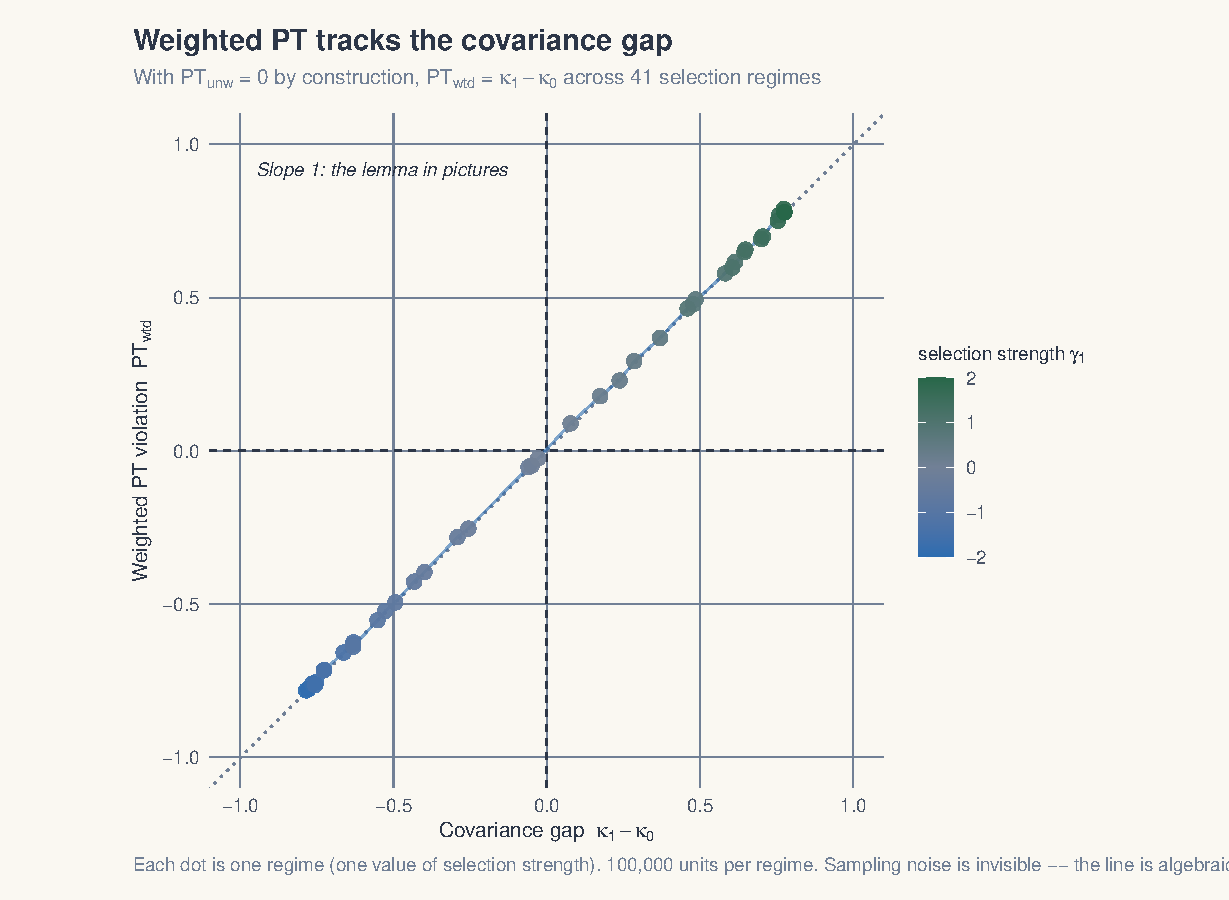
\includegraphics[width=0.78\linewidth,height=0.70\textheight,keepaspectratio]{figures/weighted_pt_covgap.pdf}
\end{center}
\vspace{-0.4em}
\begin{center}
\footnotesize\color{warmgray}\itshape
$N{=}100{,}000$, $\text{PT}_{\text{unw}}=0$ by construction. Sweep selection strength $\gamma_1$ from $-2$ to $+2$.\\
\highlight{$\text{PT}_{\text{wtd}}$ traces $\kappa_1 - \kappa_0$ exactly.}\; Slope 1. Not a regularity --- an identity.
\end{center}
\end{frame}

%% ---------- W7: Implications — not a robustness check ----------
\begin{frame}{Weighted vs unweighted is \textit{not} a robustness check}
\vspace{0.4em}
\begin{itemize}\small
  \item Running both and hoping they agree is \textit{not} a robustness check --- it's a comparison of two different estimands under two different assumptions.
  \item Disagreement is information about the \highlight{covariance gap}, not about whether DiD ``works.''
  \item Pick the parameter your question demands. Then defend the corresponding PT.
\end{itemize}
\vspace{0.6em}
\begin{block}{So what do you do?}
\small
Event studies (next!) interrogate \textit{which} PT you can defend. You can run them weighted, unweighted, or both --- but each tests a different assumption.
\end{block}
\vspace{0.2em}
\meta{Derivation and simulation: \texttt{decks/code/Weighted-PT/weighted\_pt\_chart.R}. \\ Background: Scott's Substack, ``Diff-in-Diff, population weights and parallel trends,'' Part 1 \& 2.}
\end{frame}

%% =====================================================================
%%                                LESSON 7
%% =====================================================================
\remixsection{7.\ Event Studies \\[0.3em] {\normalsize\normalfont as Falsifications --- and 2$\times$2s}}

%% ---------- F1: DiD is a courtroom case ----------
\begin{frame}{DiD is a courtroom case}
\vspace{0.8em}
\pullquote{Scientific theories achieve credibility not just by explaining observed phenomena, but by excluding alternative explanations.}{Scott Cunningham, \textit{The Remix} (forthcoming, Yale 2026)}
\vspace{0.6em}
\begin{itemize}
  \item You are the prosecutor. The DiD coefficient is your \highlight{claim of guilt}.
  \item A claim is not evidence. The evidence is everything you do around the claim.
  \item Popper: a theory earns credibility by deriving what \textit{else} should be true if it's right --- and testing those predictions.
\end{itemize}
\end{frame}

%% ---------- F2: Five parts of a strong DiD ----------
\begin{frame}{Five parts of a strong DiD}
\vspace{0.6em}
\begin{enumerate}
  \item \textbf{\color{accent}Bite} --- the policy actually changed what it was supposed to change
  \item \textbf{\color{accent}Event study} --- pre/post coefficients around treatment
  \item \textbf{\color{accent}Falsification} --- run a rival theory on a placebo group or outcome and try to reject \textit{it}
  \item \textbf{\color{accent}Main result} --- the DiD on the actual outcome
  \item \textbf{\color{accent}Mechanism} --- the causal pathway from $D$ to $Y$
\end{enumerate}
\vspace{0.5em}
\meta{The point estimate alone is a case ``so weak that readers and the public are justified to reject it.''}
\end{frame}

%% ---------- F3: Falsification — rival theory on trial ----------
\begin{frame}{A falsification puts a rival theory on trial}
\vspace{0.5em}
Write down what \textit{else} the rival theory would predict --- something irrelevant to your treatment --- and test it.
\vspace{0.6em}
\begin{itemize}
  \item \highlight{Same outcome, alternative groups.} A group your treatment shouldn't reach, but the rival would. \\
  \meta{Min wage on low-wage employment? Re-run on higher-wage workers.}
  \item \highlight{Same group, alternative outcomes.} Outcomes your treatment shouldn't move, but the rival would. \\
  \meta{Cigarette tax on smoking-related hospitalizations? Re-run on appendicitis and fractures.}
\end{itemize}
\vspace{0.5em}
\meta{Failing to reject the rival's prediction weakens the rival --- it never \textit{confirms} you. That's the Popperian asymmetry.}
\end{frame}

%% ---------- F4: A punchline — Cohen-Cole and Fletcher ----------
\begin{frame}{A clean falsification: peer effects on height}
\vspace{0.6em}
\begin{itemize}
  \item Christakis \& Fowler (2007): peer-effect contagion in obesity
  \item Cohen-Cole \& Fletcher (2008): re-run the same model on \highlight{height, acne, and headaches}
  \item All three show ``contagion''
\end{itemize}
\vspace{1em}
\pullquote{We have not been able to become taller by having tall friends.}{Cohen-Cole \& Fletcher, paraphrased}
\vspace{0.4em}
\meta{The result isn't necessarily wrong. But the empirical model is suspect.}
\end{frame}

%% ---------- F5: Bridge to event study ----------
\begin{frame}{The event study is the falsification built into the timeline}
\vspace{0.5em}
\begin{itemize}
  \item Every coefficient at $\tau = -2, -3, \ldots, -q$ asks the same question: \\
  \textit{Is something already moving the treated group relative to controls, before $D$ turned on?}
  \item That's a rival theory. The pre-period coefficients are its placebo test.
  \item This one is built into the regression. The others (placebo group, placebo outcome) you have to construct.
\end{itemize}
\vspace{0.4em}
\meta{None of these falsifications is the whole case. Event study, placebo group, placebo outcome --- each rules out a different rival theory. \textit{Together they are powerful.}}
\end{frame}

%% ---------- Slide 50: Event study is 2x2 in motion ----------
\begin{frame}{An event study is the 2$\times$2 viewed in motion}
\vspace{0.6em}
\begin{itemize}
  \item Instead of one pre-period and one post-period, use \textit{many}
  \item Estimate a separate effect at each event-time relative to treatment
  \item Plot them as a sequence: $\hat{\beta}_{-4}, \hat{\beta}_{-3}, \ldots, \hat{\beta}_{-1}, \hat{\beta}_{0}, \hat{\beta}_{+1}, \ldots$
  \item The graph tells two stories: \highlight{pre-trends} (left of zero) and \highlight{dynamics} (right of zero)
\end{itemize}
\end{frame}

%% ---------- Slide 51: The saturated regression ----------
\begin{frame}{Every coefficient is a 2$\times$2 against $t = -1$}
\vspace{0.6em}
The saturated event-study regression:
\vspace{0.2em}
\[
Y_{it} \;=\; \alpha_i + \lambda_t + \sum_{k \neq -1} \beta_k \cdot \mathbf{1}\{\text{event time}_{it} = k\} \cdot D_i \;+\; \varepsilon_{it}
\]

\vspace{0.8em}
\begin{center}
\Large \highlight{Drop $k = -1$ as the reference.}
\end{center}

\vspace{0.4em}
\begin{center}
\small\color{warmgray}\itshape Every other $\hat\beta_k$ is then a 2$\times$2 DiD between event-time $k$ and the period just before treatment. \;Let's prove it numerically.
\end{center}
\end{frame}

%% ---------- Slide 51b: Toy data ----------
\begin{frame}{A tiny panel where you can do the math in your head}
\footnotesize
\textbf{Cell means $\overline{Y}_{g,t}$.} \;Two treated units (T), two controls (C). \;Treatment turns on at event-time $0$.
\vspace{0.4em}
\begin{center}
\renewcommand{\arraystretch}{1.2}
\begin{tabular}{@{}lccccc@{}}
\toprule
\textbf{Event time $k$} & $-3$ & $-2$ & $-1$ & $0$ & $+1$ \\
\midrule
\textbf{Treated} \;$\overline{Y}^T_k$ & $7$ & $8$ & $9$ & $13$ & $16$ \\
\textbf{Control} \;$\overline{Y}^C_k$ & $2$ & $3$ & $4$ & $5$ & $6$ \\
\midrule
$\overline{Y}^T_k - \overline{Y}^C_k$ & $5$ & $5$ & $5$ & $8$ & $10$ \\
\bottomrule
\end{tabular}
\end{center}

\vspace{0.5em}
\begin{itemize}\setlength\itemsep{2pt}
  \item Pre-period: T--C gap is constant at $5$. \;\highlight{Parallel trends.}
  \item True ATT$(0) = 3$, \;True ATT$(+1) = 5$.
\end{itemize}
\end{frame}

%% ---------- Slide 51c: Every β̂_k by hand against t=-1 ----------
\begin{frame}{Each $\hat\beta_k$ by hand --- one formula, four answers}
\footnotesize
The 2$\times$2 against $t = -1$: \;$\hat\beta_k \;=\; (\overline{Y}^T_k - \overline{Y}^T_{-1}) - (\overline{Y}^C_k - \overline{Y}^C_{-1})$

\vspace{0.5em}
\begin{center}
\renewcommand{\arraystretch}{1.5}
\begin{tabular}{@{}lll@{}}
\toprule
\textbf{$k$} & \textbf{Calculation} & \textbf{$\hat\beta_k$} \\
\midrule
$-3$ & $(7 - 9) - (2 - 4) \;=\; -2 - (-2)$ & $\mathbf{0}$ \\
$-2$ & $(8 - 9) - (3 - 4) \;=\; -1 - (-1)$ & $\mathbf{0}$ \\
$0$  & $(13 - 9) - (5 - 4) \;=\; 4 - 1$    & $\mathbf{3}$ \\
$+1$ & $(16 - 9) - (6 - 4) \;=\; 7 - 2$    & $\mathbf{5}$ \\
\bottomrule
\end{tabular}
\end{center}

\vspace{0.5em}
\begin{center}
\small\color{warmgray}\itshape Same arithmetic each row. Pre $\to$ zeros (PT holds). Post $\to$ the true ATT.
\end{center}
\end{frame}

%% ---------- Slide 51d: Same numbers via OLS in R ----------
\begin{frame}[fragile]{Same numbers via OLS in R}
\vspace{0.5em}
\begin{lstlisting}[language=R,basicstyle=\ttfamily\small]
library(fixest)
feols(Y ~ i(event_time, treat, ref = -1) | unit + period,
      data = toy)
\end{lstlisting}

\vspace{0.6em}
\begin{center}
\renewcommand{\arraystretch}{1.2}
\begin{tabular}{@{}lc@{}}
\toprule
\textbf{coefficient} & \textbf{estimate} \\
\midrule
\texttt{event\_time::-3:treat} & $0$ \\
\texttt{event\_time::-2:treat} & $0$ \\
\texttt{event\_time::0:treat}  & $3$ \\
\texttt{event\_time::1:treat}  & $5$ \\
\bottomrule
\end{tabular}
\end{center}

\vspace{0.5em}
\begin{center}
\small\color{warmgray}\itshape OLS matches the manual 2$\times$2s to machine epsilon. The regression \textit{is} the formula.
\end{center}
\end{frame}

%% ---------- Slide 51e: Different hinge, different question ----------
\begin{frame}{You could have picked a different hinge}
\footnotesize
Re-compute $\hat\beta_{-3}$, but with $t = -2$ as the baseline:
\vspace{-0.2em}
\[
\tilde\beta_{-3} \;=\; (\overline{Y}^T_{-3} - \overline{Y}^T_{-2}) - (\overline{Y}^C_{-3} - \overline{Y}^C_{-2}) \;=\; (7 - 8) - (2 - 3) \;=\; \mathbf{0}
\]

\vspace{0.4em}
And the post-period one with $t = -2$ as the baseline:
\vspace{-0.2em}
\[
\tilde\beta_{0} \;=\; (\overline{Y}^T_{0} - \overline{Y}^T_{-2}) - (\overline{Y}^C_{0} - \overline{Y}^C_{-2}) \;=\; (13 - 8) - (5 - 3) \;=\; \mathbf{3}
\]

\vspace{0.6em}
\begin{block}{What OLS \textit{can't} give you simultaneously}
A single regression drops \textit{one} event-time dummy. \;Multicollinearity won't let it report 2$\times$2s against both $t = -1$ \textit{and} $t = -2$ at once. \;The convention is $t = -1$. \;It's a choice, not math.
\end{block}
\end{frame}

%% ---------- Slide 51f: Implication for PT falsification ----------
\begin{frame}{Why the hinge matters for parallel-trends tests}
\vspace{0.4em}
The pre-period coefficients $\hat\beta_{-q}, \ldots, \hat\beta_{-2}$ are:
\vspace{-0.2em}
\[
\hat\beta_k \;=\; \underbrace{(\overline{Y}^T_k - \overline{Y}^T_{-1})}_{\text{long-difference, treated}} \;-\; \underbrace{(\overline{Y}^C_k - \overline{Y}^C_{-1})}_{\text{long-difference, control}}
\]

\vspace{0.4em}
\begin{itemize}\setlength\itemsep{4pt}
  \item These are \textit{long-difference trends from $t = -1$} --- not point-to-point changes.
  \item If you use them as a \highlight{parallel-trends falsification}, you're testing that those long-difference trends are zero.
  \item The post-period coefficients use the \textit{same hinge}. \;The falsification model must match the long-difference structure of the post-period model.
\end{itemize}

\vspace{0.3em}
\meta{Match the model, match the test. \;A different baseline is a different question.}
\end{frame}

%% ---------- Slide 53: Live in R ----------
\begin{frame}[fragile]{castle.dta event study, live}
\vspace{0.3em}
\begin{lstlisting}[language=R]
library(fixest); library(ggplot2)
df <- read_dta("castle.dta")
df <- df %>% mutate(event_time = year - effyear)

es <- feols(l_homicide ~ i(event_time, ref = -1) | sid + year,
            data = df, cluster = ~sid)

iplot(es, main = "Event study: castle.dta")
\end{lstlisting}
\vspace{0.4em}
\meta{Full script: \texttt{CI-2/Lab/Basic-DiD/simple\_eventstudy.R}}
\end{frame}

%% =====================================================================
%%   Closing example: Miller, Johnson & Wherry (2021 QJE)
%%   Medicaid expansion and near-elderly mortality — walk through ALL the
%%   figures: 3 bite measures, 1 falsification, 1 main result, 1 summary.
%%   Placed BEFORE "What pre-trends do and don't tell us" so the meta-lesson
%%   crystallizes what the toy (castle) + the real paper (MJW) both showed.
%% =====================================================================

%% ---------- W-1: the paper, the question ----------
\begin{frame}{A closing example: Medicaid expansion and mortality}
\vspace{0.4em}
\textbf{Miller, Johnson \& Wherry (2021),} \textit{Quarterly Journal of Economics}.
\vspace{0.5em}
\begin{itemize}
  \item Did the ACA Medicaid expansion (2014) reduce mortality among the \highlight{near-elderly} (55--64)?
  \item Comparison: states that expanded vs.\ states that didn't, before vs.\ after 2014.
  \item Why \textit{near}-elderly? Because everyone 65+ has Medicare --- Medicaid expansion is irrelevant for them. \\ The elderly become a natural \highlight{placebo group} living in the same economies.
\end{itemize}
\vspace{0.5em}
\begin{block}{Walkthrough}
\small
We'll see the \highlight{bite} (three measures), the \highlight{falsification} (elderly placebo), and the \highlight{main mortality event study}. That's five figures. They build the case in sequence --- not in parallel.
\end{block}
\end{frame}

%% ---------- W-2: Bite #1 — Medicaid take-up ----------
\begin{frame}{Bite \#1: Medicaid take-up jumped in expansion states}
\begin{center}
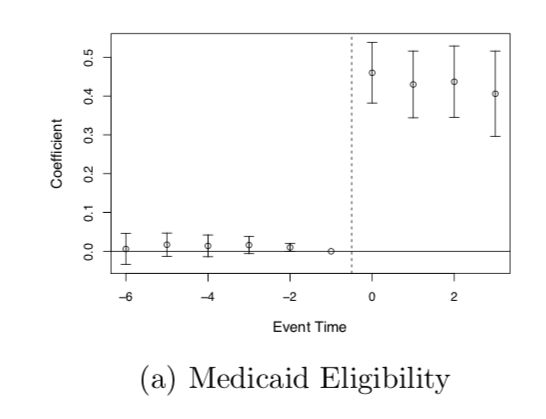
\includegraphics[height=0.60\textheight,keepaspectratio]{figures/Miller_Medicaid1.png}
\end{center}
\vspace{-0.2em}
\begin{center}
\footnotesize\color{warmgray}\itshape
\highlight{Did the policy actually move people onto Medicaid?}\; Yes --- enrollment rose sharply in expansion states post-2014, flat in non-expansion. \\
Without bite, there's no story. The mandate has to actually \textit{do} something before we can attribute downstream changes to it.
\end{center}
\end{frame}

%% ---------- W-3: Bite #2 — any insurance coverage ----------
\begin{frame}{Bite \#2: any-insurance coverage rose}
\begin{center}
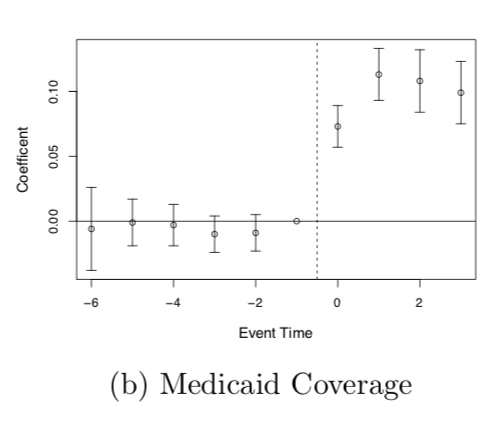
\includegraphics[height=0.62\textheight,keepaspectratio]{figures/Miller_Medicaid2.png}
\end{center}
\vspace{-0.2em}
\begin{center}
\footnotesize\color{warmgray}\itshape
\highlight{Did the new Medicaid enrollees actually gain coverage they didn't have?}\; Or did they just shift from private to Medicaid? \\
Any-insurance coverage rose --- the expansion brought in the previously uninsured, not the already-insured.
\end{center}
\end{frame}

%% ---------- W-4: Bite #3 — uninsured rate ----------
\begin{frame}{Bite \#3: the uninsured rate fell}
\begin{center}
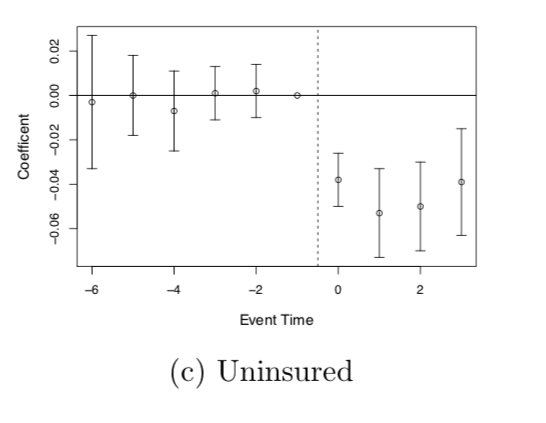
\includegraphics[height=0.62\textheight,keepaspectratio]{figures/Miller_Medicaid3.png}
\end{center}
\vspace{-0.2em}
\begin{center}
\footnotesize\color{warmgray}\itshape
\highlight{The mirror image of Bite \#2.}\; Uninsured rate dropped sharply in expansion states post-2014. \\
Three measures (Medicaid up, any-insurance up, uninsured down) converge on the same conclusion: \highlight{the policy bit.}
\end{center}
\end{frame}

%% ---------- W-5: the falsification — elderly as placebo ----------
\begin{frame}{Falsification: same model, on the 65+ population --- no effect}
\begin{center}
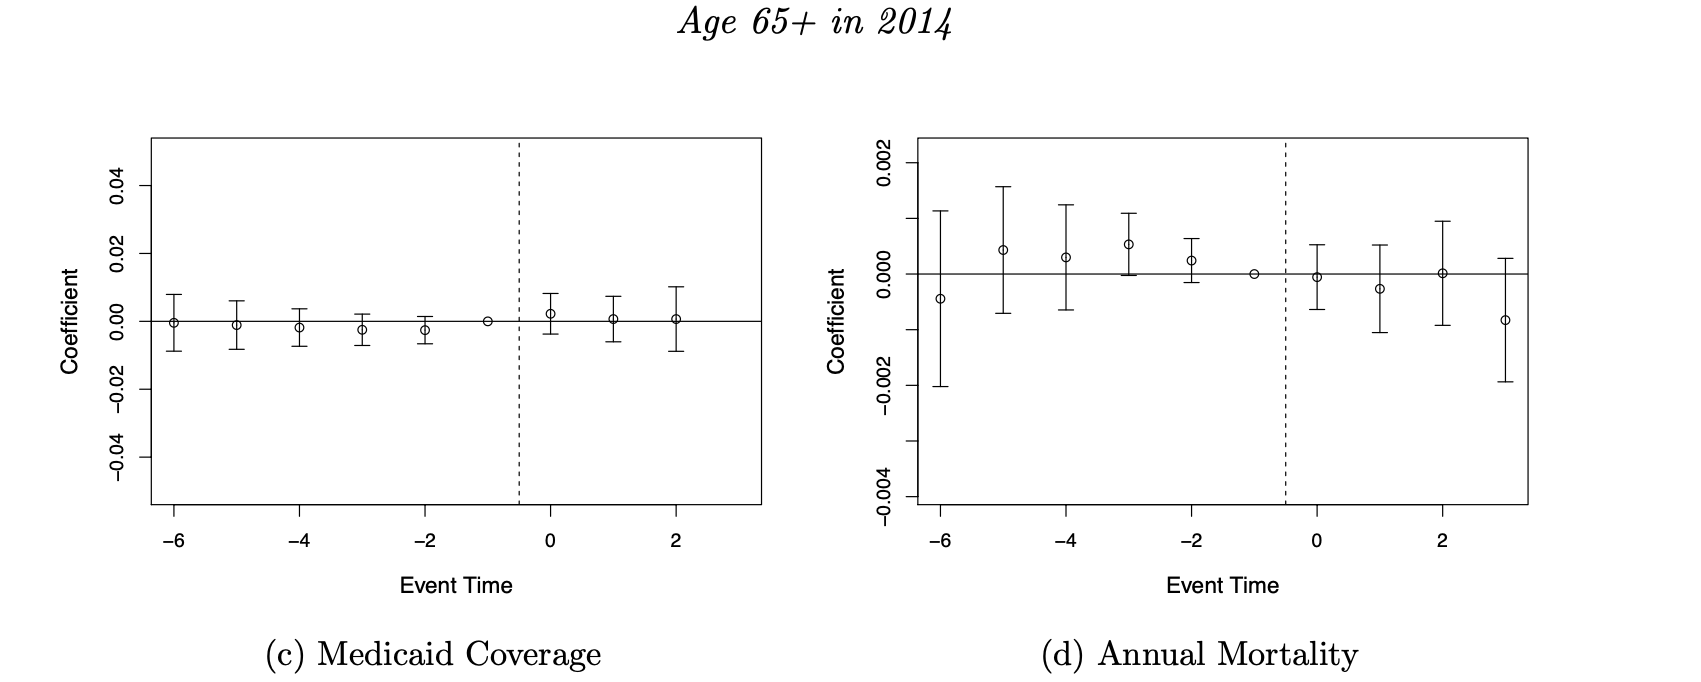
\includegraphics[height=0.60\textheight,keepaspectratio]{figures/placebo_medicaid.png}
\end{center}
\vspace{-0.2em}
\begin{center}
\footnotesize\color{warmgray}\itshape
\highlight{Same states, same years, same model --- but run on the 65+ population.}\; They all have Medicare, so Medicaid expansion shouldn't touch their mortality. \\
A rival theory (``some 2014 shock hit expansion states'') would predict a mortality effect here. It didn't appear. \highlight{Rival rejected.}
\end{center}
\end{frame}

%% ---------- W-6: the main event study ----------
\begin{frame}{The main result: $\approx 9.2\%$ reduction in near-elderly mortality}
\begin{center}
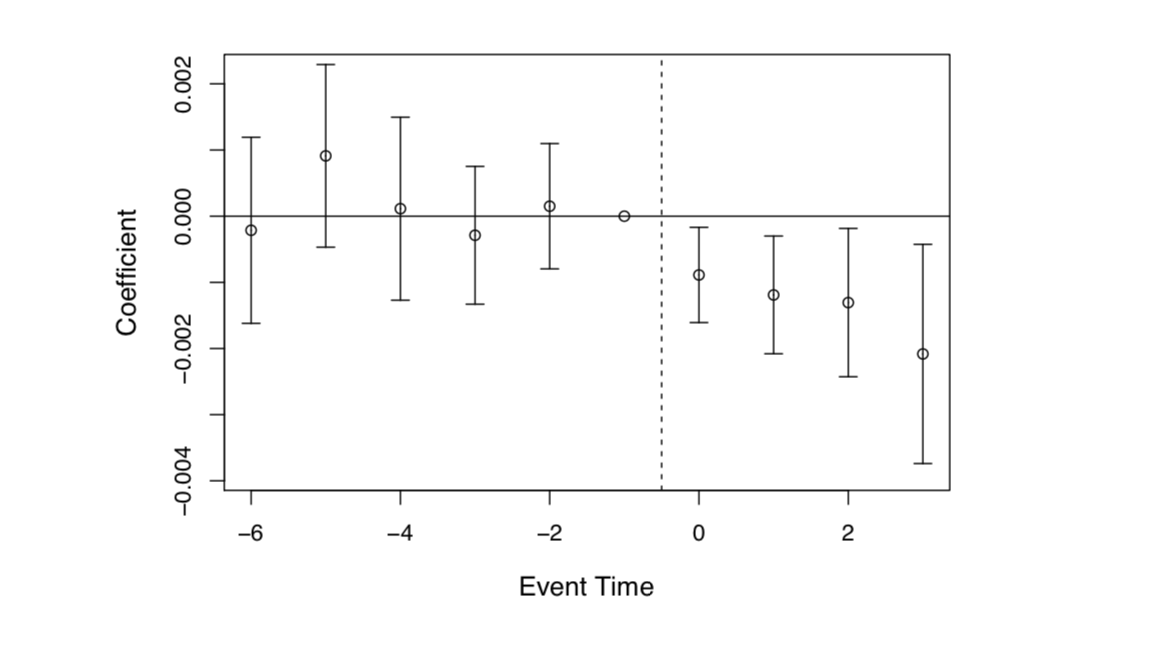
\includegraphics[height=0.62\textheight,keepaspectratio]{figures/Miller_Medicaid4.png}
\end{center}
\vspace{-0.2em}
\begin{center}
\footnotesize\color{warmgray}\itshape
Pre-trends flat. Post-2014 mortality declines in expansion states.\;\highlight{$\approx 9.2\%$ reduction.} \\
Effect \textit{grows} over time --- consistent with cumulative treatment for chronic conditions.
\end{center}
\end{frame}

%% ---------- W-7: five parts, all present ----------
\begin{frame}{The five parts of a strong DiD, all five present}
\vspace{0.4em}
\begin{center}
\renewcommand{\arraystretch}{1.45}
\footnotesize
\begin{tabular}{@{}p{0.18\textwidth} p{0.74\textwidth}@{}}
\toprule
\textbf{Bite} & Three figures: Medicaid take-up up, any-insurance up, uninsured down \\
\textbf{Event study} & Pre-trends flat; post-trends decline in expansion states \\
\textbf{Falsification} & No effect on elderly (65+) --- same states, same years, same model \\
\textbf{Main result} & $\approx 9.2\%$ reduction in mortality among the near-elderly \\
\textbf{Mechanism} & Disease-related deaths fall and compound; consistent with treated chronic conditions \\
\bottomrule
\end{tabular}
\end{center}
\vspace{0.6em}
\begin{center}
\small\color{warmgray}\itshape
None of these alone is the case. \highlight{Together they are powerful.}
\end{center}
\end{frame}

%% ---------- Slide 54: What we see ----------
\begin{frame}{What pre-trends do and don't tell us}
\vspace{0.4em}
\begin{itemize}
  \item Flat pre-trends $\rightarrow$ evidence consistent with parallel trends
  \item Sloped pre-trends $\rightarrow$ evidence \textit{against} parallel trends
  \item Flat pre-trends $\nRightarrow$ parallel trends \textit{must} hold post-treatment
  \item It's one falsification. Run the others too --- placebo groups, placebo outcomes.
  \item \highlight{Pre-trends are a gut check, not a proof.} More tomorrow (Roth-Sant'Anna, Ghanem-Sant'Anna-Wüthrich).
\end{itemize}
\end{frame}

%% ---------- Slide 55: Shiny app ----------
\begin{frame}{Try it yourself: the Event-Study Explorer}
\vspace{0.3em}
\begin{block}{Open in your browser (runs entirely client-side via shinylive)}
\centering
\href{https://scunning1975.github.io/event-study/}{\color{ocean}\texttt{scunning1975.github.io/event-study/}}
\end{block}
\vspace{0.4em}
Five sliders. Watch the event-study coefficients trace the truth in real time.
\vspace{0.4em}
\begin{itemize}\small
  \item Set the \textbf{true treatment effect} (level) and \textbf{effect slope}. Watch the post-period coefs trace the staircase.
  \item Add a \textbf{pre-trend slope}. \;\highlight{Watch the pre-period coefs slope away from zero --- the failed gut-check, visible.}
  \item Crank up the \textbf{noise} or shrink the \textbf{number of units}. \;Watch the CIs blow out.
\end{itemize}
\vspace{0.4em}
\meta{Source: \texttt{decks/code/Event-Study-Demo/app.R}. Single-cohort DiD with TWFE event study. Day 2 introduces the staggered version.}
\end{frame}

%% =====================================================================
%%                                ACT III
%% =====================================================================

%% ---------- Slide 56: Recap ----------
\begin{frame}{What we've done today}
\vspace{0.3em}
\begin{enumerate}
  \item Three founders, one design --- four averages, three subtractions
  \item Three regressions, one answer
  \item Potential outcomes, target parameters, and parallel trends
  \item Standard errors: when robust isn't robust enough
  \item The minimum wage wars
  \item Two ATTs, two parallel trends --- a callback to weighting
  \item Event studies as falsifications and 2$\times$2s
\end{enumerate}
\end{frame}

%% ---------- Slide 56b: Lab — LaLonde on experimental data ----------
\begin{frame}{Lab tonight: LaLonde (1986) on the experimental sample}
\vspace{0.4em}
\textbf{Goal.} Take every Day-1 tool and run it on real data, by hand.
\vspace{0.4em}
\begin{itemize}\small
  \item Data: NSW experimental panel from Dehejia \& Wahba (2002). Years 1974, 1975, 1978. Outcome: real earnings.
  \item Part 1: 2$\times$2 by hand on \texttt{75} $\rightarrow$ \texttt{78}.
  \item Part 2: three regressions return the same number.
  \item Part 3: event study with \texttt{75} as the baseline.
  \item Part 4: event study \textit{by hand} --- each coefficient is a 2$\times$2 against \texttt{75}.
  \item Part 5: pre-trend gut check on \texttt{74}, interpretation.
\end{itemize}
\vspace{0.4em}
\meta{Walkthrough: \texttt{glasgow/labs/Lalonde/Day1\_README.md}. \;Data link in the README. \;Reference scripts: \texttt{lalonde-did.R}, \texttt{lalonde-did-stata.do} (use the no-covariates portions only).}
\end{frame}

%% ---------- Slide 57: Preview tomorrow ----------
\begin{frame}{Tomorrow: when the 2$\times$2 stops working}
\vspace{0.4em}
\begin{itemize}
  \item Covariates --- IPW, OR, doubly robust
  \item Time-varying covariates (Caetano \& Callaway)
  \item Triple differences (Ortiz-Villavicencio \& Sant'Anna)
  \item Staggered adoption --- Goodman-Bacon, Callaway-Sant'Anna, Sun-Abraham, BJS
\end{itemize}
\end{frame}

%% ---------- Slide 58: THE CLOSING ----------
\begin{frame}[plain]
\begin{tikzpicture}[remember picture,overlay]
\fill[cream] (current page.south west) rectangle (current page.north east);
\node[anchor=center, text width=0.82\paperwidth, align=center, text=charcoal] at (current page.center) {%
  \fontsize{20pt}{26pt}\selectfont
  DiD is a research design with two ingredients ---\\[0.4em]
  the {\color{accent}\bfseries 2$\times$2 calculation} and {\color{accent}\bfseries parallel trends}.\\[0.6em]
  Together they identify the ATT.
};
\draw[accent, line width=1pt] ([yshift=2.5cm,xshift=0.25\paperwidth]current page.south west) -- ([yshift=2.5cm,xshift=-0.25\paperwidth]current page.south east);
\end{tikzpicture}
\end{frame}

\end{document}
